\documentclass{notes}

\title{A model of navigation history}
\author{Connor G. Brewster \and Alan Jeffrey}
\date{DRAFT of 2016-06-24}
\indicia{
  
\includegraphics[height=4.5ex]{images/by}
  \begin{tabular}[b]{@{}l}%
    Copyright Connor G. Brewster and Alan Jeffrey\\
    Licensed under Creative Commons License CC-BY
  \end{tabular}
}

\usepackage{amssymb}
\usepackage{graphicx}
\usepackage{float}
\usepackage{subcaption}
\usepackage{tikz}
\usetikzlibrary{fit}

% Macros, so we can change notation easily
\newcommand{\aNH}{H}
\newcommand{\Docs}{D}
\newcommand{\Active}{A}
\newcommand{\FullyActive}{F\!A}
\newcommand{\parentOf}{\rightarrow}
\newcommand{\parentOfActive}{\twoheadrightarrow}
\newcommand{\childOf}{\larrow}
\newcommand{\activeChildOf}{\twoheadleftarrow}
\newcommand{\leChron}{\le}
\newcommand{\ltChron}{<}
\newcommand{\geChron}{\ge}
\newcommand{\gtChron}{>}
\newcommand{\eqSess}{\sim}
\newcommand{\ltSess}{\lesssim}
\newcommand{\gtSess}{\gtrsim}
\newcommand{\rootDoc}{d_0}
\newcommand{\aDoc}{d}
\newcommand{\bDoc}{e}
\newcommand{\cDoc}{f}
\newcommand{\st}{\mathbin.}
\newtheorem{goal}{Goal}
\newtheorem{patch}{Patch}
\newtheorem{counterexample}{Counterexample}
\newtheorem{experiment}{Experiment}

\tikzstyle{doc} = [draw=black, fill=blue!10, circle, font={\normalfont\sffamily}]
\tikzstyle{fully} = [draw=red, thick]
\tikzstyle{active} = [color=white, fill=blue!50!black]
\tikzstyle{jshactive} = [active] % ASAJ: if we want jshactive to be distinct [fill=green!50]

\begin{document}

\maketitle

\subparagraph{Abstact:}
Navigation has been a core component of the web since its inception:
users and scripts can follow hyperlinks, or can go back or forwards
through the session history. Despite its long existence, navigation
history has no formal model or properties. In this paper, we present a
formal model aligned with the \textsc{whatwg} specification of navigation
history, and investigate its properties. The fundamental property of
navigation history is that traversing the history by $\delta$
then by $\delta'$ should be the same as traversing by
$\delta+\delta'$. In particular, traversing by $+1$ (forward) then by
$-1$ (back) is the same as traversing by $0$ (doing nothing). We show
that the specification-aligned model does not satisfy this property,
by exhibiting a series of counter-examples, which motivate three
patches to the model. The patched model is homomorphic. We present a
series of experiments, showing that browsers are inconsistent in their
implementation of navigation history, but that their behaviour is
closer to the patched model than to the specification-aligned
model. We propose patches to the specification to align it with the
homomorphic model.

\subparagraph{ACM Classification:}
D.2.1 Requirements/Specifications.

\subparagraph{Keywords:}
Formal model,
Navigation,
Session history,
Specification,
Web browsers.

\section{Introduction}

Navigation has been a core component of the web since its inception:
users and scripts can follow hyperlinks, or can go back or forwards
through the session history. Users are exposed to this functionality
through following hyperlinks, and by the forward and back buttons.
Scripts have many ways of accessing session history, via the
navigation API~\cite[\S7.7]{whatwg} and the \verb|element.click()| method.

Despite its long existence, navigation history has no formal model or
properties. The specification of the navigation API is informal, and
has complex dependencies on the rest of the HTML
specification~\cite{whatwg}. There is little discussion of the goals
of the API, and an unclear alignment with browser implementations.

In this paper, we present a formal model of navigation, aligned with
the HTML specification, and investigate its properties. The
starting point is that there is a total order of
\emph{documents}\footnote{%
  We are eliding some of the technical details of the specification here,
  in particular we are conflatating a \emph{browsing context}
  with the document it contains, and we are ignoring issues around
  document loading and unloading.
}, one of which is \emph{active}, for example:
\[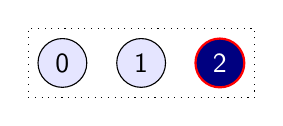
\begin{tikzpicture}
  \node[doc](0) at (0,0){0};
  \node[doc](1) at (1,0){1};
  \node[doc,jshactive,fully](2) at (2,0){2};
  \node[draw,dotted,fit=(0)(1)(2)] {};
\end{tikzpicture}\]
In diagrams, we use left-to-right order to indicate order,
and highlight the active document. The user can \emph{traverse}
the history which changes the active document, for example pressing
the back button:
\[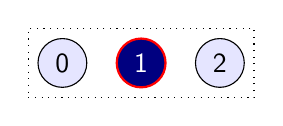
\begin{tikzpicture}
  \node[doc](0) at (0,0){0};
  \node[doc,jshactive,fully](1) at (1,0){1};
  \node[doc](2) at (2,0){2};
  \node[draw,dotted,fit=(0)(1)(2)] {};
\end{tikzpicture}\]
The user can also \emph{navigate}, which replaces any document
after the currently active document by a fresh document:
\[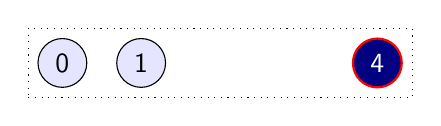
\begin{tikzpicture}
  \node[doc](0) at (0,0){0};
  \node[doc](1) at (1,0){1};
  \node[doc,jshactive,fully](4) at (4,0){4};
  \node[draw,dotted,fit=(0)(1)(4)] {};
\end{tikzpicture}\]
Users can also traverse the history by more than one document
at a time, for example by using a pull-down menu from the back
or forwards button. This is called \emph{traversing by $\delta$},
for instance we can traverse our running example by $-2$
to get:
\[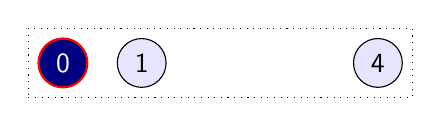
\begin{tikzpicture}
  \node[doc,jshactive,fully](0) at (0,0){0};
  \node[doc](1) at (1,0){1};
  \node[doc](4) at (4,0){4};
  \node[draw,dotted,fit=(0)(1)(4)] {};
\end{tikzpicture}\]
We formalize the notions of traversal and navigation in
\S\ref{sec:model}, and show that they satisfy two pleasant
properties:
\begin{itemize}

\item \emph{traverse-then-traverse}:
  traversing by $\delta$ then by $\delta'$
  is the same as traversing by $\delta+\delta'$.
  
\item \emph{navigate-then-traverse}:
  navigating then traversing by $-1$
  has the original active document.
  
\end{itemize}
Thus far, the model is refreshingly simple, and corresponds well to
the specification and to browser implmentations. Where the problems
arise is in the \emph{hierarchical} nature of documents. HTML
documents can contain \verb|iframe| elements, which
are independent documents in their own right, often
used to embed third party content such as advertisements.
We can treat each document as a tree, for example:
\[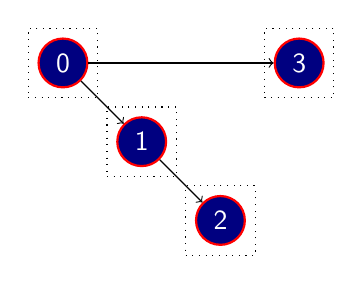
\begin{tikzpicture}
  \node[doc,jshactive,fully](0) at (0,0){0};
  \node[doc,active,fully](1) at (1,-1){1};
  \node[doc,active,fully](2) at (2,-2){2};
  \node[doc,active,fully](3) at (3,0){3};
  \node[draw,dotted,fit=(0)] {};
  \node[draw,dotted,fit=(1)] {};
  \node[draw,dotted,fit=(2)] {};
  \node[draw,dotted,fit=(3)] {};
  \draw[->](0)--(1);
  \draw[->](1)--(2);
  \draw[->](0)--(3);
\end{tikzpicture}\]
The problem comes from the ability of each document to
navigate separately and maintain its own session history,
but that traversal is a global operation that operates
on the \emph{joint session history}. For example
if document $2$ in the previous example navigates, the
resulting state is:
\[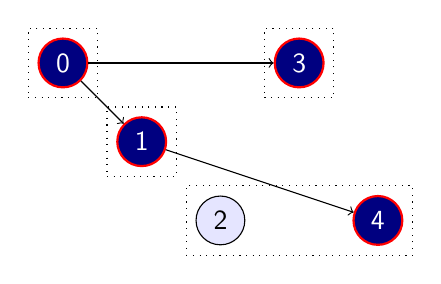
\begin{tikzpicture}
  \node[doc,active,fully](0) at (0,0){0};
  \node[doc,active,fully](1) at (1,-1){1};
  \node[doc](2) at (2,-2){2};
  \node[doc,active,fully](3) at (3,0){3};
  \node[doc,jshactive,fully](4) at (4,-2){4};
  \node[draw,dotted,fit=(0)] {};
  \node[draw,dotted,fit=(1)] {};
  \node[draw,dotted,fit=(2)(4)] {};
  \node[draw,dotted,fit=(3)] {};
  \draw[->](0)--(1);
  \draw[->](1)--(4);
  \draw[->](0)--(3);
\end{tikzpicture}\]
and then if document $1$ navigates, the state is:
\[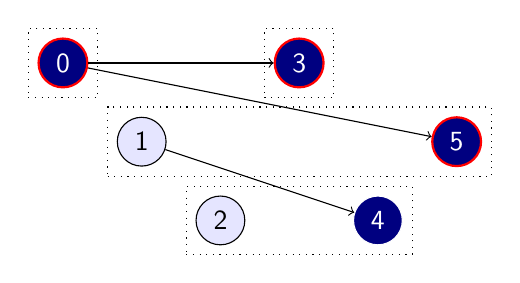
\begin{tikzpicture}
  \node[doc,active,fully](0) at (0,0){0};
  \node[doc](1) at (1,-1){1};
  \node[doc](2) at (2,-2){2};
  \node[doc,active,fully](3) at (3,0){3};
  \node[doc,active](4) at (4,-2){4};
  \node[doc,jshactive,fully](5) at (5,-1){5};
  \node[draw,dotted,fit=(0)] {};
  \node[draw,dotted,fit=(1)(5)] {};
  \node[draw,dotted,fit=(2)(4)] {};
  \node[draw,dotted,fit=(3)] {};
  \draw[->](0)--(5);
  \draw[->](1)--(4);
  \draw[->](0)--(3);
\end{tikzpicture}\]
Note that node $4$ here is in an unusual state: it is active, but has
an inactive ancestor. The specification~\cite[\S7.7]{whatwg}
distinguishes between \emph{active} documents such as $4$, and
\emph{fully active} documents such as $0$, $3$ and $5$. Active
documents can become fully active by traversals involving their
ancestors. For example, after traversing by $-1$, document $4$ is
fully active:
\[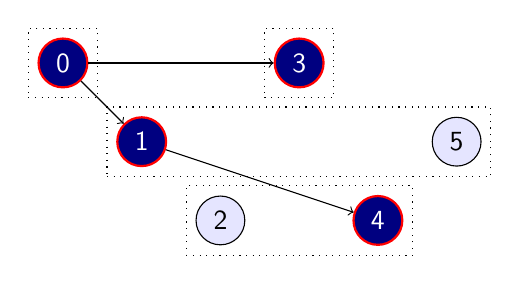
\begin{tikzpicture}
  \node[doc,active,fully](0) at (0,0){0};
  \node[doc,jshactive,fully](1) at (1,-1){1};
  \node[doc](2) at (2,-2){2};
  \node[doc,active,fully](3) at (3,0){3};
  \node[doc,active,fully](4) at (4,-2){4};
  \node[doc](5) at (5,-1){5};
  \node[draw,dotted,fit=(0)] {};
  \node[draw,dotted,fit=(1)(5)] {};
  \node[draw,dotted,fit=(2)(4)] {};
  \node[draw,dotted,fit=(3)] {};
  \draw[->](0)--(1);
  \draw[->](1)--(4);
  \draw[->](0)--(3);
\end{tikzpicture}\]
As even a simple example like this shows, the combination of features
quickly results in a complex mix of session history, ordering, and
document hierarchy, which leads to the problems:
\begin{itemize}

\item \emph{Formally} there is no simple model,
  and the model provided by the specification does
  not satisfy the traverse-then-traverse property.

\item \emph{Experimentally} the browsers disagree
  with each other, and with the HTML specification,
  about the semantics of navigation.

\end{itemize}
In this paper, we address these:
\begin{itemize}

\item \S\ref{sec:model} provides a formal model of navigation history,
  which is intended to align with the specification. We show, through
  a series of examples, that it does not satisfy the
  traverse-then-traverse property, and give patches to the model for
  each example. The final model does satisfy the
  traverse-then-traverse property.

\item \S\ref{sec:experiments} investigates how well the patched
  model aligns with existing browser implementations. We show
  ways in which the browsers exhibit behaviours which are not
  aligned with the specification, and discuss how our proposed
  model matches these behaviours.

\end{itemize}
Finally, we propose changed wording to the specification, which
would bring it in line with our patched model.

\section{Preliminaries}

[Define forest, tree, root, total order, equivalence.]

\section{Model}
\label{sec:model}

A \emph{navigation history} $\aNH=(\Docs,\Active,{\parentOf},{\leChron},{\eqSess})$ consists of:
\begin{itemize}
\item a set $\Docs$ (the \emph{documents}),
\item a subset $\Active \subseteq \Docs$ (the \emph{active} documents),
\item a forest $(\Docs,{\parentOf})$ (the \emph{document hierarchy}),
\item a total order $(\Docs,{\leChron})$ (the \emph{chronological order}), and
\item an equivalence relation $(\Docs,{\eqSess})$ (the \emph{same-session equivalence}).
\end{itemize}
such that:
\begin{itemize}
\item for every $\aDoc$ there is a unique $\aDoc'\in\Active$ such that $\aDoc \eqSess \aDoc'$,
\item for every $\aDoc \parentOf \bDoc \eqSess \bDoc'$
  we have $\aDoc \parentOf \bDoc'$, and
\item for every $\aDoc \parentOf \bDoc$, we have $\aDoc \leChron \bDoc$.
\end{itemize}
Define:
\begin{itemize}
\item $\rootDoc$ is the unique active root document,
\item $\aDoc \parentOfActive \bDoc$ when $\aDoc \parentOf \bDoc$ and $\bDoc \in \Active$,
\item $\FullyActive = \{ \aDoc \mid \rootDoc \parentOfActive^* \aDoc \}$
  (the \emph{fully active} documents),
\item $\aDoc \ltSess \bDoc$ whenever $\aDoc \eqSess \bDoc$ and $\aDoc \ltChron \bDoc$,
\item the \emph{session future} of $\aDoc$ is $\{ \bDoc \mid \aDoc \ltSess \bDoc \}$,
\item the \emph{session past} of $\aDoc$ is $\{ \bDoc \mid \aDoc \gtSess \bDoc \}$,
\item the \emph{joint session future} is $\{ \bDoc \mid \exists \aDoc \in \FullyActive \st \aDoc \ltSess \bDoc \}$,
\item the \emph{joint session past} is $\{ \bDoc \mid \exists \aDoc \in \FullyActive \st \aDoc \gtSess \bDoc \}$,
\end{itemize}
Define \emph{deleting $\aDoc$ from $\aNH$}, when $\aDoc\not\in\FullyActive$, to be $\aNH'$ where:
\begin{itemize}
\item $\Docs' = \aDoc \setminus \{ \bDoc \mid \aDoc\parentOf^* \bDoc \}$,
\item $\bDoc\in\Active'$ whenever $\bDoc\in\Active$,
\item $\bDoc\leChron'\cDoc$ whenever $\bDoc\leChron\cDoc$,
\item $\bDoc\parentOf'\cDoc$ whenever $\bDoc\parentOf\cDoc$, and
\item $\bDoc\eqSess'\cDoc$ whenever $\bDoc\eqSess\cDoc$.
\end{itemize}
Define \emph{replacing $\aDoc$ by $\aDoc'$ in $\aNH$}, where $\aDoc\in\Active$ and
$\aDoc'\notin\Docs$, to be $\aNH'$ where:
\begin{itemize}
\item $\Docs' = \Docs \cup \{\aDoc'\}$,
\item $\bDoc \in \Active'$ whenever
  $\bDoc \in \Active$ and $\bDoc\ne\aDoc$, or
  $\bDoc=\aDoc'$,
\item $\bDoc \leChron' \cDoc$ whenever
  $\bDoc \leChron \cDoc$, or $\cDoc = \aDoc'$,
\item $\bDoc \parentOf' \cDoc$ whenever
  $\bDoc \parentOf \cDoc$, or
  $\bDoc \parentOf \aDoc$ and $\cDoc = \aDoc'$, and
\item $\bDoc \eqSess' \cDoc$ whenever
  $\bDoc \eqSess \cDoc$, or
  $\bDoc \eqSess \aDoc$ and $\cDoc = \aDoc'$, or
  $\aDoc \eqSess \cDoc$ and $\bDoc = \aDoc'$.
\end{itemize}
Define \emph{navigating from $\aDoc$ to $\aDoc'$ in $\aNH$} to be the result of:
\begin{itemize}
\item deleting the session future of $\aDoc$, and
\item replacing $\aDoc$ by $\aDoc'$.
\end{itemize}
Define \emph{traversing the history to $\aDoc$ in $\aNH$} to be $\aNH'$ where:
\begin{itemize}
\item $\Docs'$ is $\Docs$,
\item $\bDoc\in\Active'$ whenever $\aDoc\not\eqSess\bDoc \in \Active$, or
  $\aDoc=\bDoc$,
\item $\bDoc\leChron'\cDoc$ whenever $\bDoc\leChron\cDoc$,
\item $\bDoc\parentOf'\cDoc$ whenever $\bDoc\parentOf\cDoc$, and
\item $\bDoc\eqSess'\cDoc$ whenever $\bDoc\eqSess\cDoc$.
\end{itemize}
Define \emph{$\aNH$ traverses the history by $+\delta$ to $\aNH'$} when:
\begin{itemize}
\item the joint session future of $\aNH$ is $\aDoc_1 \gtChron \cdots \gtChron \aDoc_\delta \gtChron \cdots$,
\item $H$ traverses the history to $d_\delta$ in $H'$
\end{itemize}
Define \emph{$\aNH$ traverses the history by $-\delta$ to $\aNH'$} when:
\begin{itemize}
\item the joint session past of $\aNH$ is $\aDoc_1 \ltChron \cdots \ltChron \aDoc_\delta \ltChron \cdots$,
\item $H$ traverses the history to $d_\delta$ in $H'$
\end{itemize}
Define \emph{$\aNH$ traverses the history by $0$ to $\aNH'$} when $\aNH=\aNH'$.

[This defn is meant to align with the spec.]

\section{Properties}


[State some goals, e.g. go($\delta$);go($\delta'$) is the same as go($\delta+\delta'$),
  navigate;go($-1$) has the same fully active documents as doing nothing,
  session history can be implemented effeciently in memory...]

[I suspect none of these are true of the current spec, can we find a model in which
  they are true?]

\begin{goal}
\label{goal:homomorphism}
  If $H$ traverses the history by $\delta$ to $H'$
  and $H'$ traverses the history by $\delta'$ to $H''$
  then $H$ traverses the history by $\delta+\delta'$ to $H''$.
\end{goal}

\begin{counterexample}
  \label{counterexample:homomorphism1}
  Let $H$ be:
  \[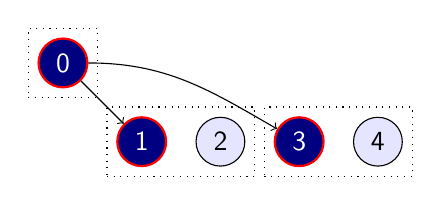
\begin{tikzpicture}
    \node[doc,active,fully](0) at (0,0){0};
    \node[doc,jshactive,fully](1) at (1,-1){1};
    \node[doc](2) at (2,-1){2};
    \node[doc,active,fully](3) at (3,-1){3};
    \node[doc](4) at (4,-1){4};
    \node[draw,dotted,fit=(0)] {};
    \node[draw,dotted,fit=(1)(2)] {};
    \node[draw,dotted,fit=(3)(4)] {};
    \draw[->](0)--(1);
    \draw[->](0)to[out=0,in=150](3);
  \end{tikzpicture}\]
  which traverses the history by $1$ to:
  \[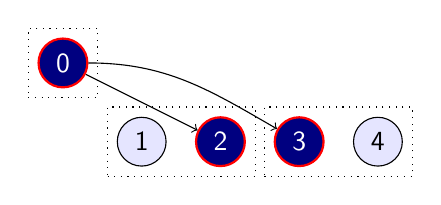
\begin{tikzpicture}
    \node[doc,active,fully](0) at (0,0){0};
    \node[doc](1) at (1,-1){1};
    \node[doc,jshactive,fully](2) at (2,-1){2};
    \node[doc,active,fully](3) at (3,-1){3};
    \node[doc](4) at (4,-1){4};
    \node[draw,dotted,fit=(0)] {};
    \node[draw,dotted,fit=(1)(2)] {};
    \node[draw,dotted,fit=(3)(4)] {};
    \draw[->](0)--(2);
    \draw[->](0)to[out=0,in=150](3);
  \end{tikzpicture}\]
  which traverses the history by $1$ to:
  \[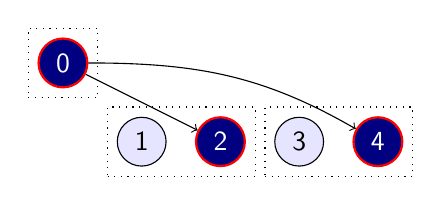
\begin{tikzpicture}
    \node[doc,active,fully](0) at (0,0){0};
    \node[doc](1) at (1,-1){1};
    \node[doc,active,fully](2) at (2,-1){2};
    \node[doc](3) at (3,-1){3};
    \node[doc,jshactive,fully](4) at (4,-1){4};
    \node[draw,dotted,fit=(0)] {};
    \node[draw,dotted,fit=(1)(2)] {};
    \node[draw,dotted,fit=(3)(4)] {};
    \draw[->](0)--(2);
    \draw[->](0)to[out=0,in=150](4);
  \end{tikzpicture}\]
  but $H$ traverses the history $2$ to:
  \[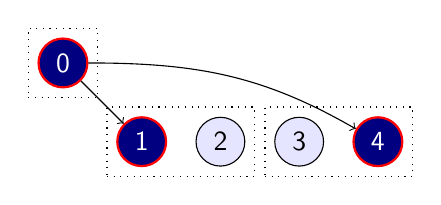
\begin{tikzpicture}
    \node[doc,active,fully](0) at (0,0){0};
    \node[doc,active,fully](1) at (1,-1){1};
    \node[doc](2) at (2,-1){2};
    \node[doc](3) at (3,-1){3};
    \node[doc,jshactive,fully](4) at (4,-1){4};
    \node[draw,dotted,fit=(0)] {};
    \node[draw,dotted,fit=(1)(2)] {};
    \node[draw,dotted,fit=(3)(4)] {};
    \draw[->](0)--(1);
    \draw[->](0)to[out=0,in=150](4);
  \end{tikzpicture}\]
\end{counterexample}
%
This counterexample is caused by the definition of `traverses the history by $\delta$' which
only traverses one document's session history. Instead, we should traverse
the history of all $\delta$ documents.

\begin{patch}
Define \emph{$\aNH$ traverses the history by $+\delta$ to $\aNH'$} when:
\begin{itemize}
\item the joint session future of $\aNH$ is $\aDoc_1 \ltChron \cdots \ltChron \aDoc_\delta \ltChron \cdots$,
\item there is some $\aNH=\aNH_0,\ldots,\aNH_\delta=\aNH'$, such that
\item $H_{i-1}$ traverses the history to $d_i$ in $H_i$ for each $1 \le i \le \delta$.
\end{itemize}
Define \emph{$\aNH$ traverses the history by $-\delta$ to $\aNH'$} when:
\begin{itemize}
\item the joint session past of $\aNH$ is $\aDoc_1 \gtChron \cdots \gtChron \aDoc_\delta \gtChron \cdots$,
\item there is some $\aNH=\aNH_0,\ldots,\aNH_\delta=\aNH'$, such that
\item $H_{i-1}$ traverses the history to $d_i$ in $H_i$ for each $1 \le i \le \delta$.
\end{itemize}
\end{patch}
Unfortunately, Goal~\ref{goal:homomorphism} is not satisfied,
even with this patch.
\begin{counterexample}
  Let $H$ be:
  \[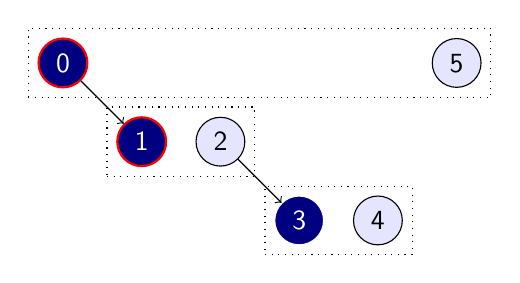
\begin{tikzpicture}
    \node[doc,active,fully](0) at (0,0){0};
    \node[doc,jshactive,fully](1) at (1,-1){1};
    \node[doc](2) at (2,-1){2};
    \node[doc,active](3) at (3,-2){3};
    \node[doc](4) at (4,-2){4};
    \node[doc](5) at (5,0){5};
    \node[draw,dotted,fit=(0)(5)] {};
    \node[draw,dotted,fit=(1)(2)] {};
    \node[draw,dotted,fit=(3)(4)] {};
    \draw[->](0)--(1);
    \draw[->](2)--(3);
  \end{tikzpicture}\]
  which moves forwards by $1$ to:
  \[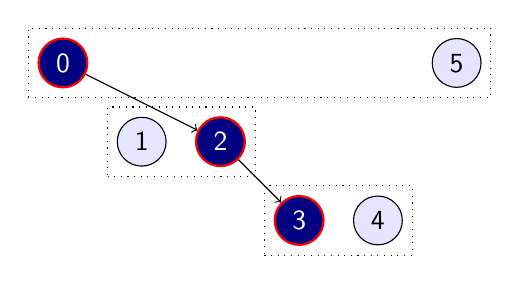
\begin{tikzpicture}
    \node[doc,active,fully](0) at (0,0){0};
    \node[doc](1) at (1,-1){1};
    \node[doc,jshactive,fully](2) at (2,-1){2};
    \node[doc,active,fully](3) at (3,-2){3};
    \node[doc](4) at (4,-2){4};
    \node[doc](5) at (5,0){5};
    \node[draw,dotted,fit=(0)(5)] {};
    \node[draw,dotted,fit=(1)(2)] {};
    \node[draw,dotted,fit=(3)(4)] {};
    \draw[->](0)--(2);
    \draw[->](2)--(3);
  \end{tikzpicture}\]
  which in turn moves forwards by $1$ to:
  \[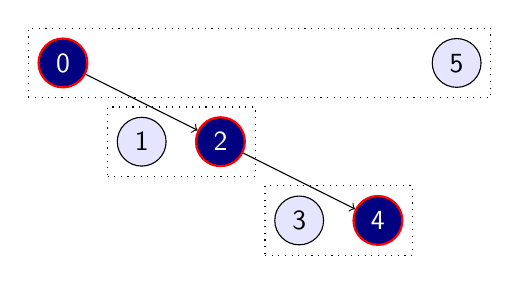
\begin{tikzpicture}
    \node[doc,active,fully](0) at (0,0){0};
    \node[doc](1) at (1,-1){1};
    \node[doc,active,fully](2) at (2,-1){2};
    \node[doc](3) at (3,-2){3};
    \node[doc,jshactive,fully](4) at (4,-2){4};
    \node[doc](5) at (5,0){5};
    \node[draw,dotted,fit=(0)(5)] {};
    \node[draw,dotted,fit=(1)(2)] {};
    \node[draw,dotted,fit=(3)(4)] {};
    \draw[->](0)--(2);
    \draw[->](2)--(4);
  \end{tikzpicture}\]
  but $H$ goes forward by $2$ to:
  \[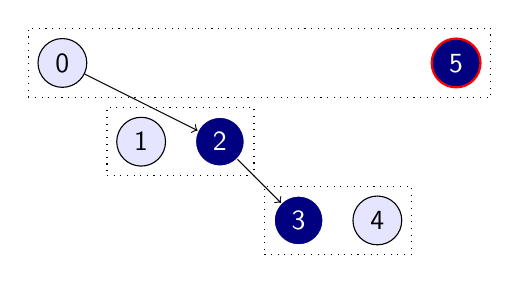
\begin{tikzpicture}
    \node[doc](0) at (0,0){0};
    \node[doc](1) at (1,-1){1};
    \node[doc,active](2) at (2,-1){2};
    \node[doc,active](3) at (3,-2){3};
    \node[doc](4) at (4,-2){4};
    \node[doc,jshactive,fully](5) at (5,0){5};
    \node[draw,dotted,fit=(0)(5)] {};
    \node[draw,dotted,fit=(1)(2)] {};
    \node[draw,dotted,fit=(3)(4)] {};
    \draw[->](0)--(2);
    \draw[->](2)--(3);
  \end{tikzpicture}\]
\end{counterexample}
The problem this time is that the definition of `joint session history' only includes
the fully active documents, not all active documents.

\begin{patch}
Define:
\begin{itemize}
\item the \emph{joint session future} is $\{ \bDoc \mid \exists \aDoc \in \Active \st \aDoc \ltSess \bDoc \}$, and
\item the \emph{joint session past} is $\{ \bDoc \mid \exists \aDoc \in \Active \st \aDoc \gtSess \bDoc \}$.
\end{itemize}
\end{patch}


\begin{counterexample}
  Let $H$ be:
  %% \[\begin{tikzpicture}
  %%   \node[doc,active,fully](0) at (0,0){0};
  %%   \node[doc](1) at (1,-1){1};
  %%   \node[doc](2) at (2,-2){2};
  %%   \node[doc,active,fully](3) at (3,-2){3};
  %%   \node[doc,jshactive,fully](4) at (4,-1){4};
  %%   \node[draw,dotted,fit=(0)]{};
  %%   \node[draw,dotted,fit=(1)(4)]{};
  %%   \node[draw,dotted,fit=(2)(3)]{};
  %%   \draw[->](0)--(4);
  %%   \draw[->](0)to[out=-20,in=120](3);
  %% \end{tikzpicture}\]
  %% which traverses the history by $-1$ to:
  \[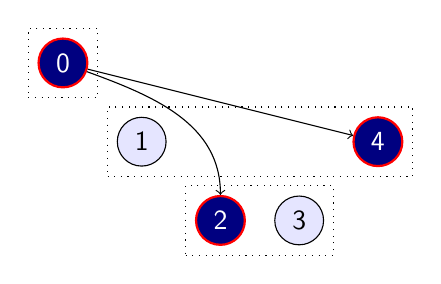
\begin{tikzpicture}
    \node[doc,active,fully](0) at (0,0){0};
    \node[doc](1) at (1,-1){1};
    \node[doc,jshactive,fully](2) at (2,-2){2};
    \node[doc](3) at (3,-2){3};
    \node[doc,active,fully](4) at (4,-1){4};
    \node[draw,dotted,fit=(0)]{};
    \node[draw,dotted,fit=(1)(4)]{};
    \node[draw,dotted,fit=(2)(3)]{};
    \draw[->](0)--(4);
    \draw[->](0)to[out=-20,in=90](2);
  \end{tikzpicture}\]
  which traverses the history by $-1$ to:
  \[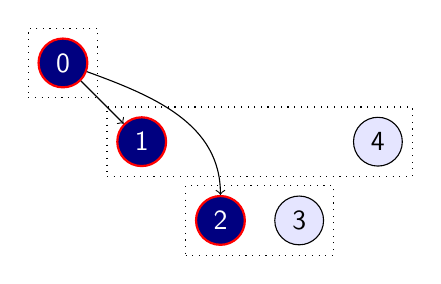
\begin{tikzpicture}
    \node[doc,active,fully](0) at (0,0){0};
    \node[doc,jshactive,fully](1) at (1,-1){1};
    \node[doc,active,fully](2) at (2,-2){2};
    \node[doc](3) at (3,-2){3};
    \node[doc](4) at (4,-1){4};
    \node[draw,dotted,fit=(0)]{};
    \node[draw,dotted,fit=(1)(4)]{};
    \node[draw,dotted,fit=(2)(3)]{};
    \draw[->](0)--(1);
    \draw[->](0)to[out=-20,in=90](2);
  \end{tikzpicture}\]
  which traverses the history by $1$ to:
  \[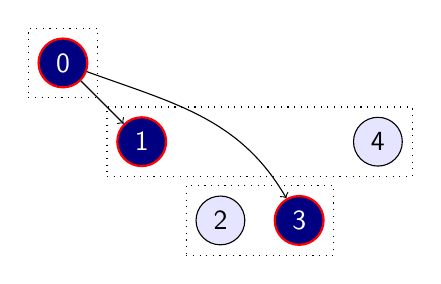
\begin{tikzpicture}
    \node[doc,active,fully](0) at (0,0){0};
    \node[doc,active,fully](1) at (1,-1){1};
    \node[doc](2) at (2,-2){2};
    \node[doc,jshactive,fully](3) at (3,-2){3};
    \node[doc](4) at (4,-1){4};
    \node[draw,dotted,fit=(0)]{};
    \node[draw,dotted,fit=(1)(4)]{};
    \node[draw,dotted,fit=(2)(3)]{};
    \draw[->](0)--(1);
    \draw[->](0)to[out=-20,in=120](3);
  \end{tikzpicture}\]
  %% which traverses the history by $1$ to:
  %% \[\begin{tikzpicture}
  %%   \node[doc,active,fully](0) at (0,0){0};
  %%   \node[doc](1) at (1,-1){1};
  %%   \node[doc](2) at (2,-2){2};
  %%   \node[doc,active,fully](3) at (3,-2){3};
  %%   \node[doc,jshactive,fully](4) at (4,-1){4};
  %%   \node[draw,dotted,fit=(0)]{};
  %%   \node[draw,dotted,fit=(1)(4)]{};
  %%   \node[draw,dotted,fit=(2)(3)]{};
  %%   \draw[->](0)--(4);
  %%   \draw[->](0)to[out=-20,in=120](3);
  %% \end{tikzpicture}\]
  which is not the same as $H$.
\end{counterexample}

[ASAJ: Not sure about this\dots]

\begin{patch}
Define \emph{$\aNH$ traverses the history from $\aDoc'$} when there is some $\aDoc$ such that:
\begin{itemize}
\item $\aDoc\ltSess\aDoc'$,
\item for any $\bDoc\ltSess\aDoc'$ we have $\bDoc\leChron\aDoc$, and
\item $\aNH$ traverses the history to $\aDoc$.
\end{itemize}
Define \emph{$\aNH$ traverses the history by $-\delta$ to $\aNH'$} when:
\begin{itemize}
\item the joint session past and active documents of $\aNH$ is $\aDoc_1 \gtChron \cdots \gtChron \aDoc_\delta \gtChron \cdots$,
\item there is some $\aNH=\aNH_0,\ldots,\aNH_\delta=\aNH'$, such that
\item $H_{i-1}$ traverses the history from $d_i$ in $H_i$ for each $1 \le i \le \delta$.
\end{itemize}
\end{patch}

\begin{goal}
  If $\aDoc$ in $\aNH$ navigates to $\aDoc'$ in $\aNH'$,
  and $\aNH'$ traverses the history by $-1$ to $\aNH''$,
  then $\FullyActive=\FullyActive''$.
\end{goal}

%% \begin{counterexample}
%%   \[\begin{tikzpicture}
%%     \node[doc,active,fully](0) at (0,0){0};
%%     \node[doc,jshactive,fully](1) at (1,-1){1};
%%     \node[doc](2) at (2,0){2};
%%     \node[draw,dotted,fit=(0)(2)] {};
%%     \node[draw,dotted,fit=(1)]{};
%%     \draw[->](0)--(1);
%%   \end{tikzpicture}\]
%%   navigates 1 to 3 in:
%%   \[\begin{tikzpicture}
%%     \node[doc,active,fully](0) at (0,0){0};
%%     \node[doc](1) at (1,-1){1};
%%     \node[doc](2) at (2,0){2};
%%     \node[doc,jshactive,fully](3) at (3,-1){3};
%%     \node[draw,dotted,fit=(0)(2)] {};
%%     \node[draw,dotted,fit=(1)(3)]{};
%%     \draw[->](0)--(3);
%%   \end{tikzpicture}\]
%%   which traverses the history by $-1$ to:
%%   \[\begin{tikzpicture}
%%     \node[doc](0) at (0,0){0};
%%     \node[doc](1) at (1,-1){1};
%%     \node[doc,jshactive,fully](2) at (2,0){2};
%%     \node[doc,active](3) at (3,-1){3};
%%     \node[draw,dotted,fit=(0)(2)] {};
%%     \node[draw,dotted,fit=(1)(3)]{};
%%     \draw[->](0)--(3);
%%   \end{tikzpicture}\]
%% \end{counterexample}

\section{Experiments}
\label{sec:experiments}

[In this section various different navigation and traversal scenarios are tested in popular web browsers to see where they differ in behaviour from both the spec and each other.]

\begin{experiment}
  In this experiment Goal~\ref{goal:homomorphism} is tested.
  \begin{itemize}
    \item \emph{$\aNH$ traverses the history by $-4$ to $\aNH'$}
    \item \emph{$\aNH'$ traverses the history by $+4$ to $\aNH''$}
  \end{itemize}
  By Goal~\ref{goal:homomorphism}, these traversals should be the same thing as \emph{$\aNH$ traversing by $0$} which is a no-op; therefore, $\aNH = \aNH''$.

  Firefox:
  \begin{figure}[H]
    \raisebox{-.5\height}{
      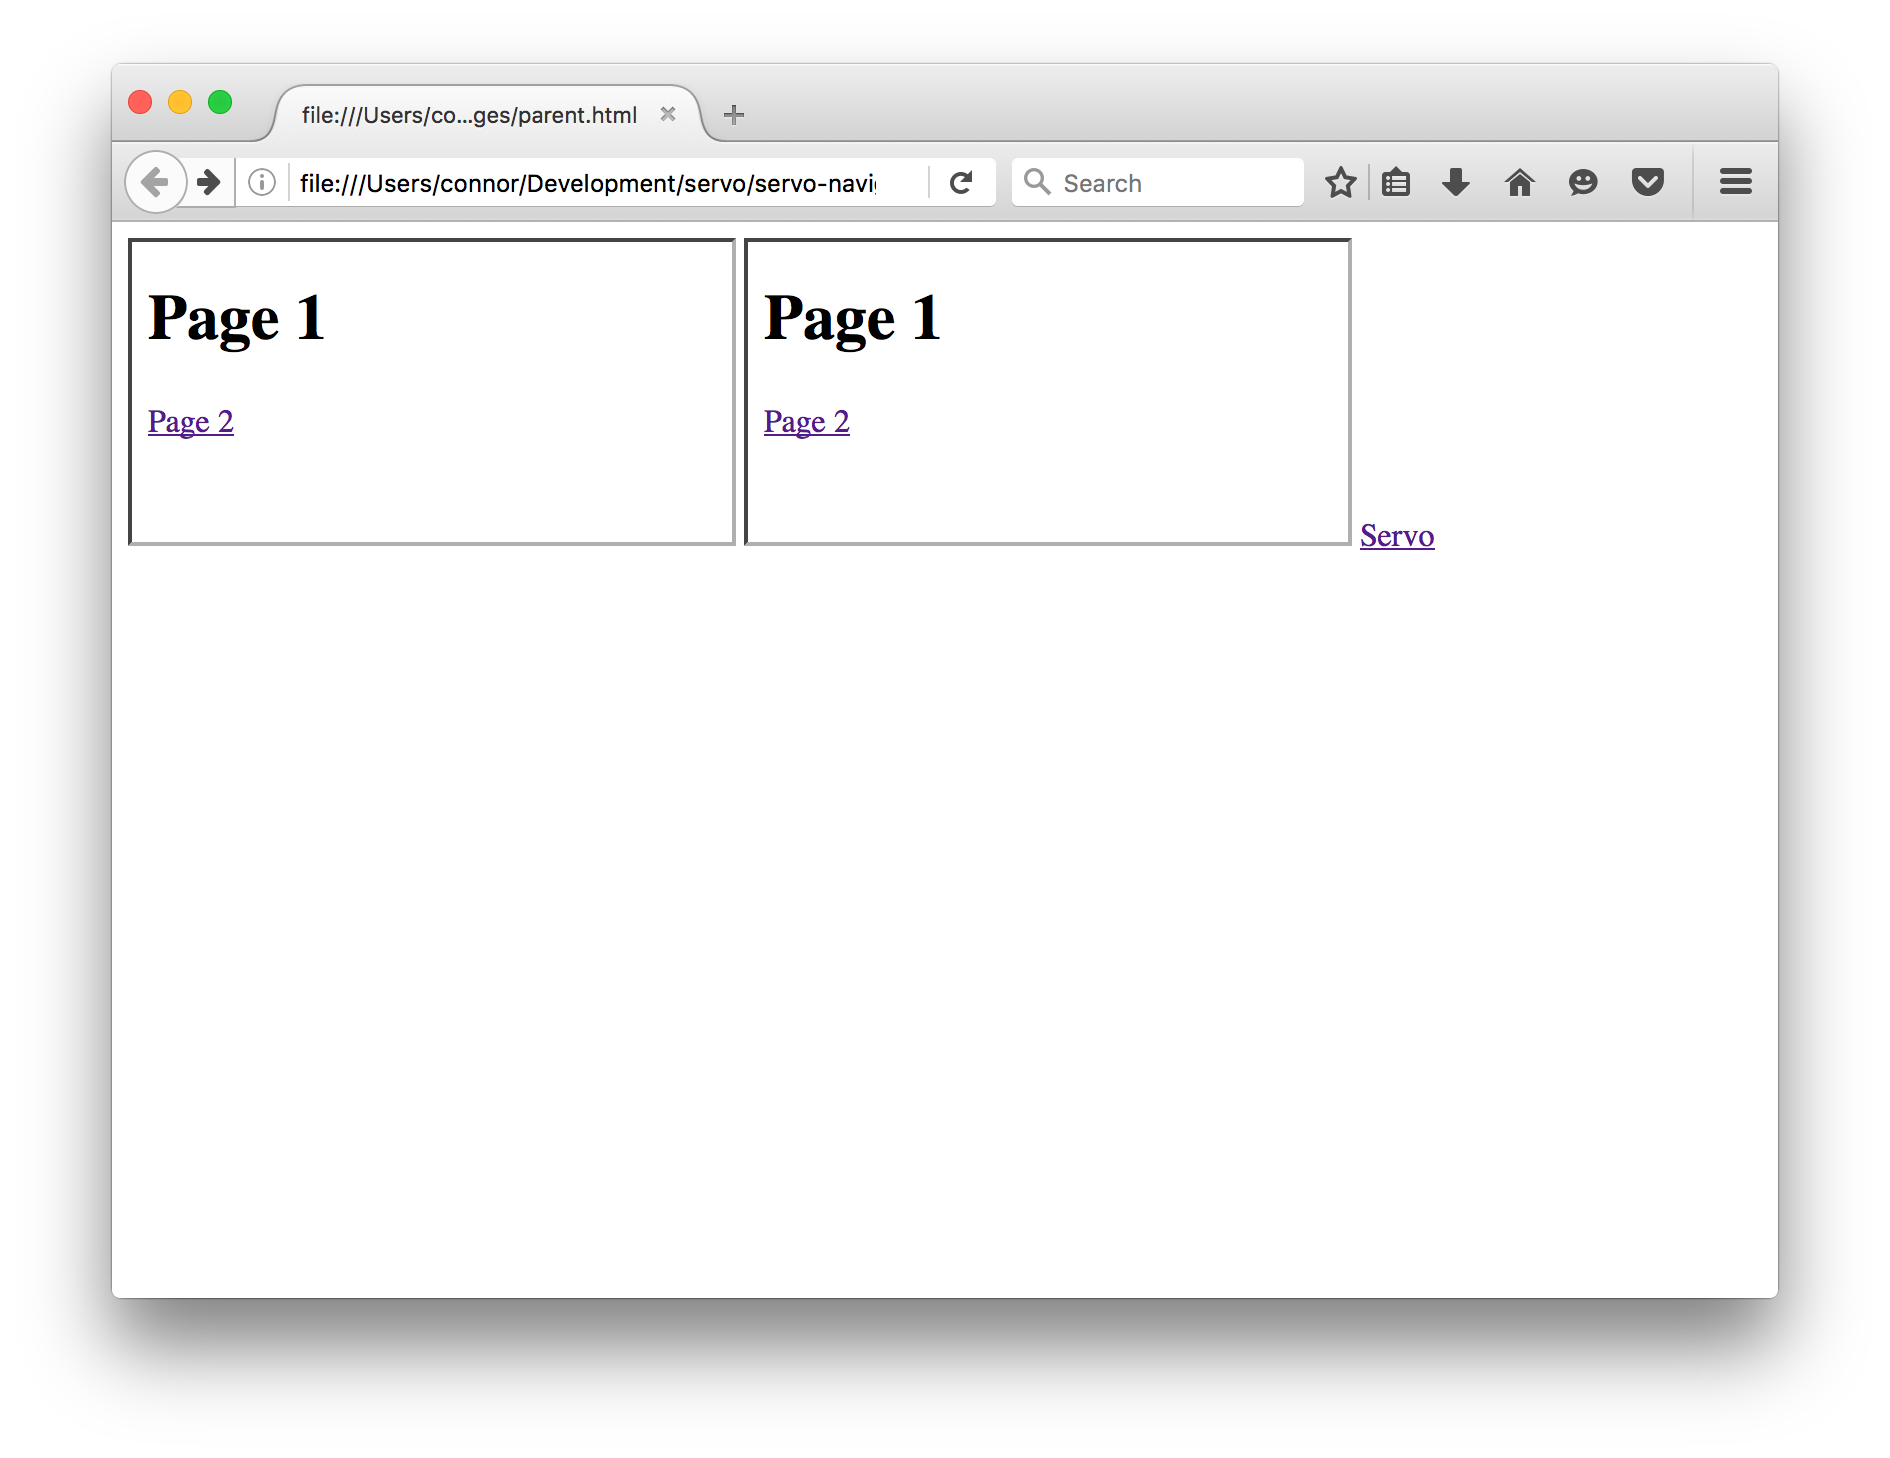
\includegraphics[width=.5\linewidth]{images/experiments/forwardback4/firefox/1.png}%
    }~\raisebox{-.5\height}{
      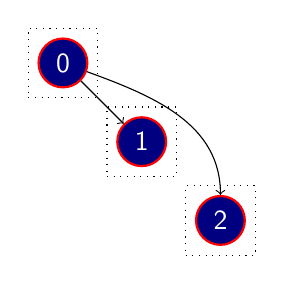
\begin{tikzpicture}
        \node[doc,active,fully](0) at (0,0){0};
        \node[doc,active,fully](1) at (1,-1){1};
        \node[doc,jshactive,fully](2) at (2,-2){2};
        \node[draw,dotted,fit=(0)]{};
        \node[draw,dotted,fit=(1)]{};
        \node[draw,dotted,fit=(2)]{};
        \draw[->](0)--(1);
        \draw[->](0)to[out=-20,in=90](2);
      \end{tikzpicture}
    }
    \caption{Initial State}
  \end{figure}

  Navigate document $1$ to Page 2:
  \begin{figure}[H]
    \raisebox{-.5\height}{
      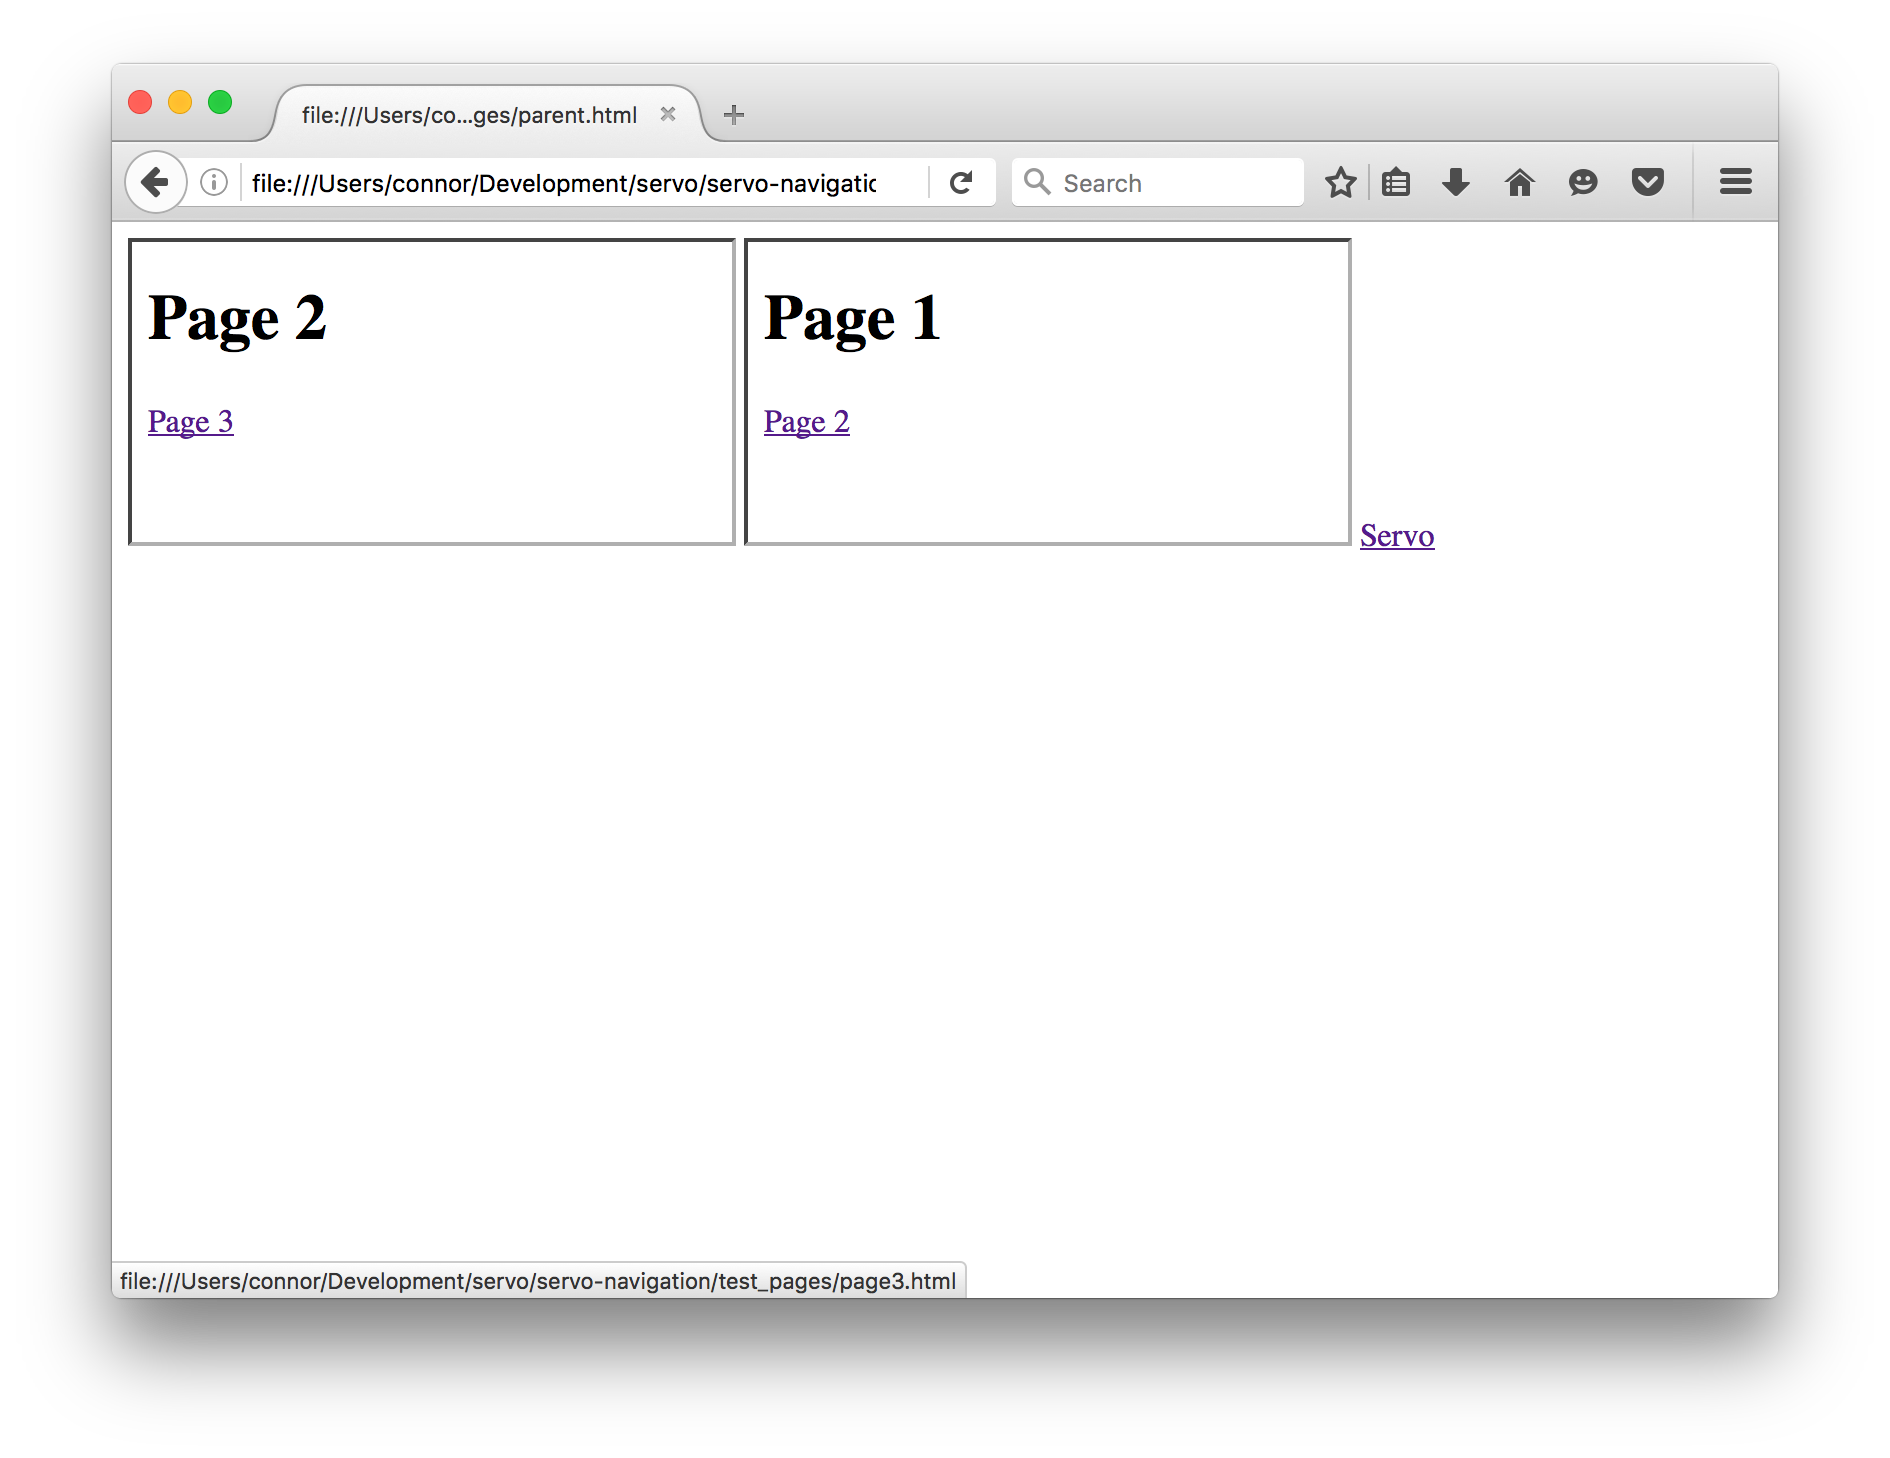
\includegraphics[width=.5\linewidth]{images/experiments/forwardback4/firefox/2.png}
    }~\raisebox{-.5\height}{
      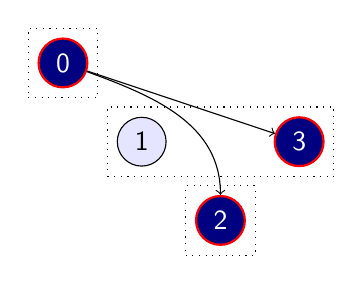
\begin{tikzpicture}
        \node[doc,active,fully](0) at (0,0){0};
        \node[doc](1) at (1,-1){1};
        \node[doc,active,fully](2) at (2,-2){2};
        \node[doc,jshactive,fully](3) at (3,-1){3};
        \node[draw,dotted,fit=(0)]{};
        \node[draw,dotted,fit=(1)(3)]{};
        \node[draw,dotted,fit=(2)]{};
        \draw[->](0)--(3);
        \draw[->](0)to[out=-20,in=90](2);
      \end{tikzpicture}
    }
    \caption{Navigate document $1$ to Page 2.}
  \end{figure}

  Navigate document $3$ to Page 3:
  \begin{figure}[H]
    \raisebox{-.5\height}{
      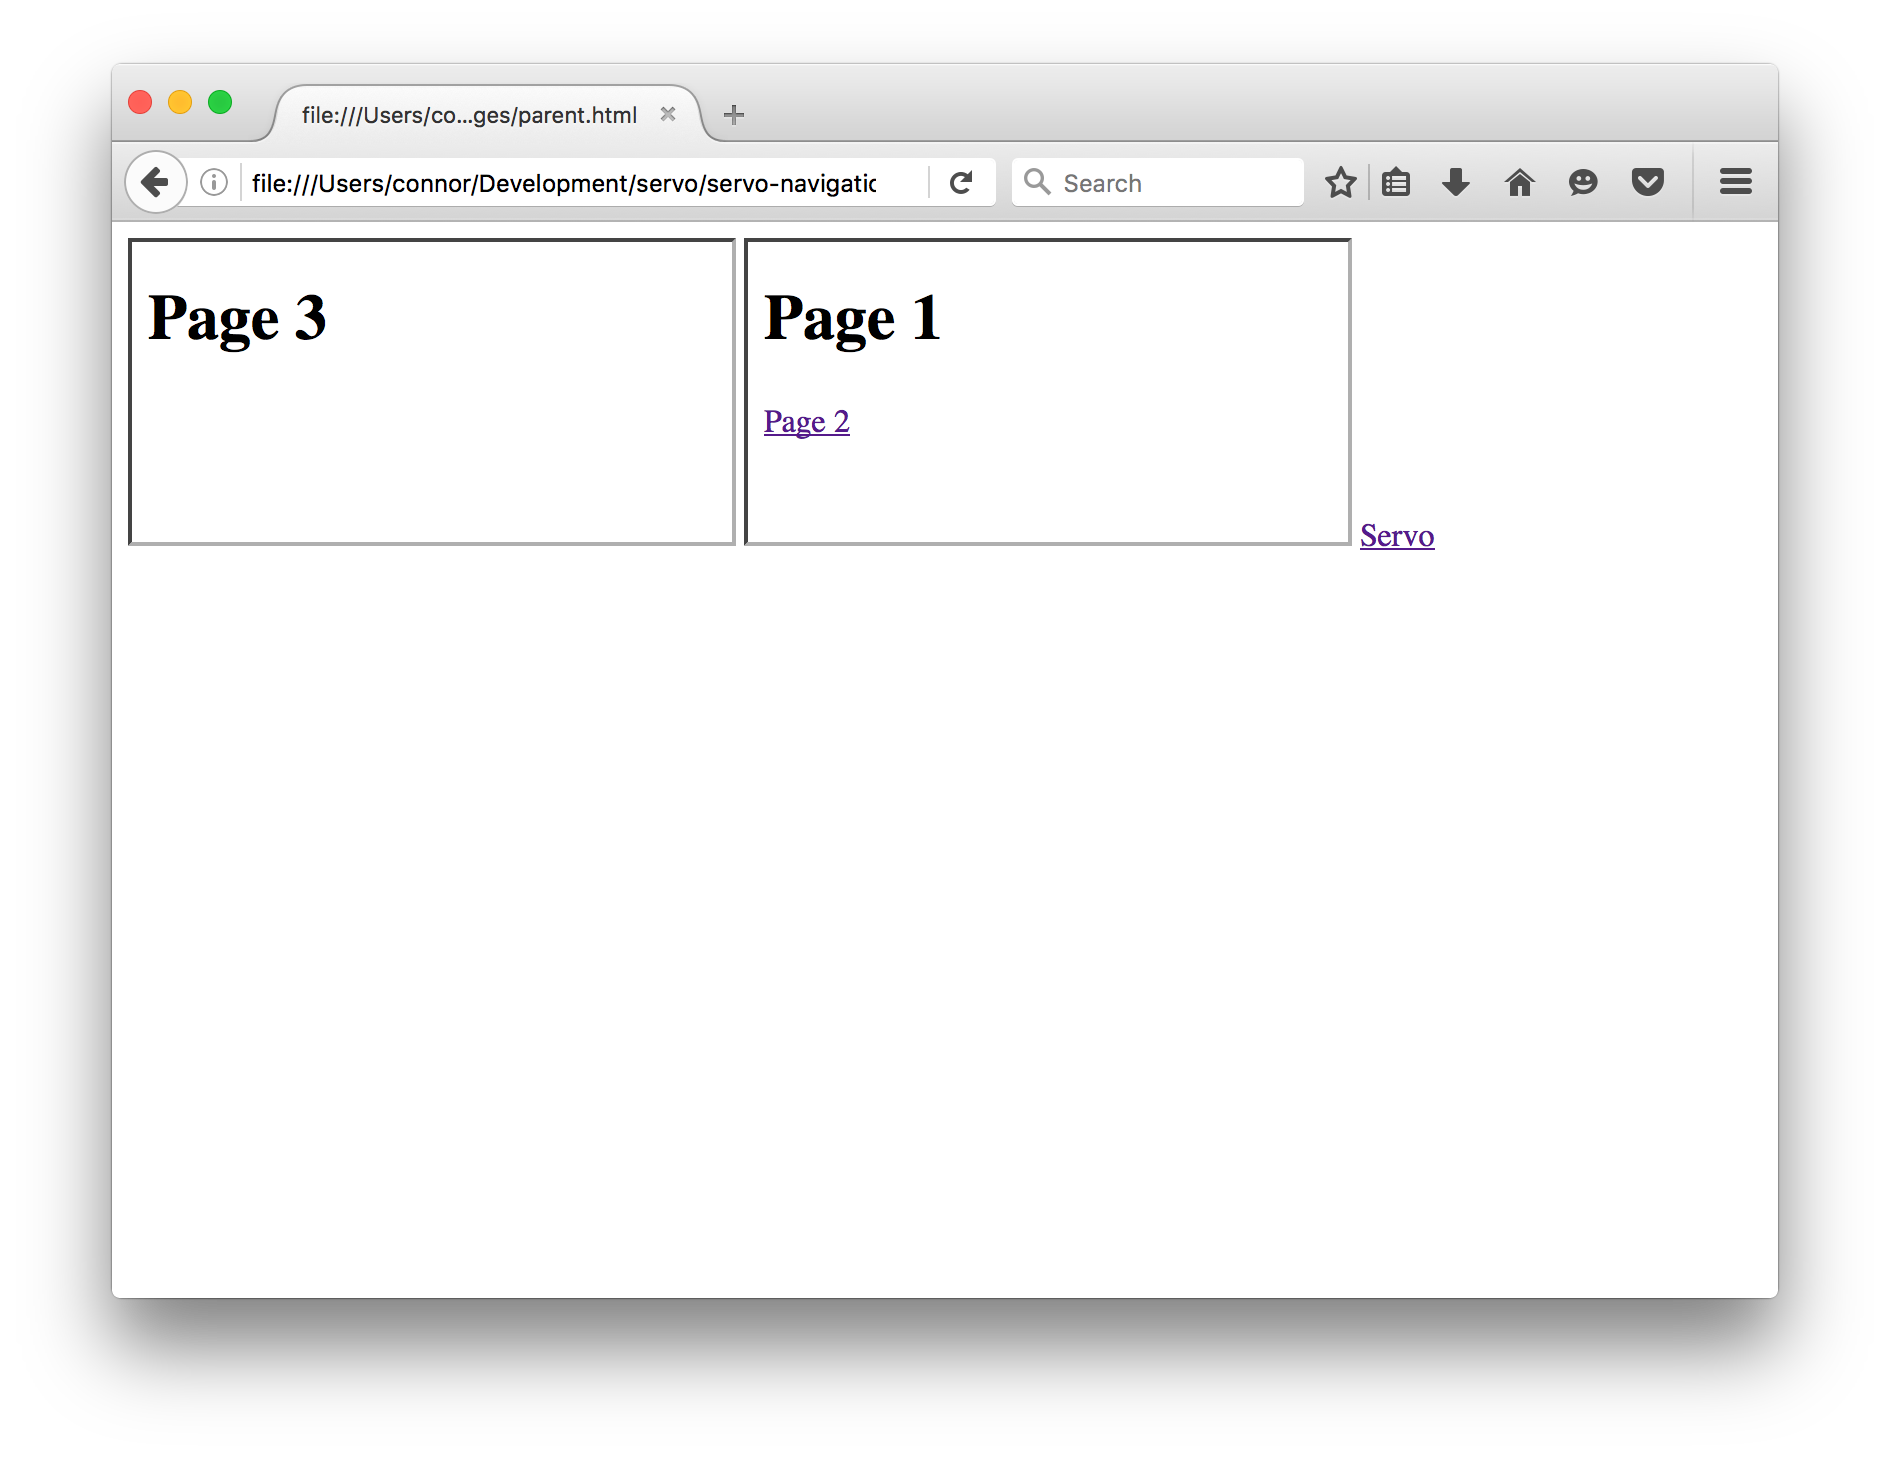
\includegraphics[width=.5\linewidth]{images/experiments/forwardback4/firefox/3.png}
    }~\raisebox{-.5\height}{
      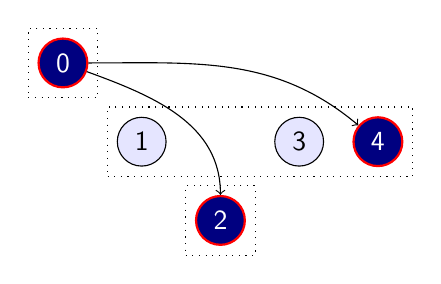
\begin{tikzpicture}
        \node[doc,active,fully](0) at (0,0){0};
        \node[doc](1) at (1,-1){1};
        \node[doc,active,fully](2) at (2,-2){2};
        \node[doc](3) at (3,-1){3};
        \node[doc,jshactive,fully](4) at (4,-1){4};
        \node[draw,dotted,fit=(0)]{};
        \node[draw,dotted,fit=(1)(4)]{};
        \node[draw,dotted,fit=(2)]{};
        \draw[->](0)to[out=0,in=140](4);
        \draw[->](0)to[out=-20,in=90](2);
      \end{tikzpicture}
    }
    \caption{Navigate document $3$ to Page 3.}
  \end{figure}

  Navigate document $2$ to Page 2:
  \begin{figure}[H]
    \raisebox{-.5\height}{
      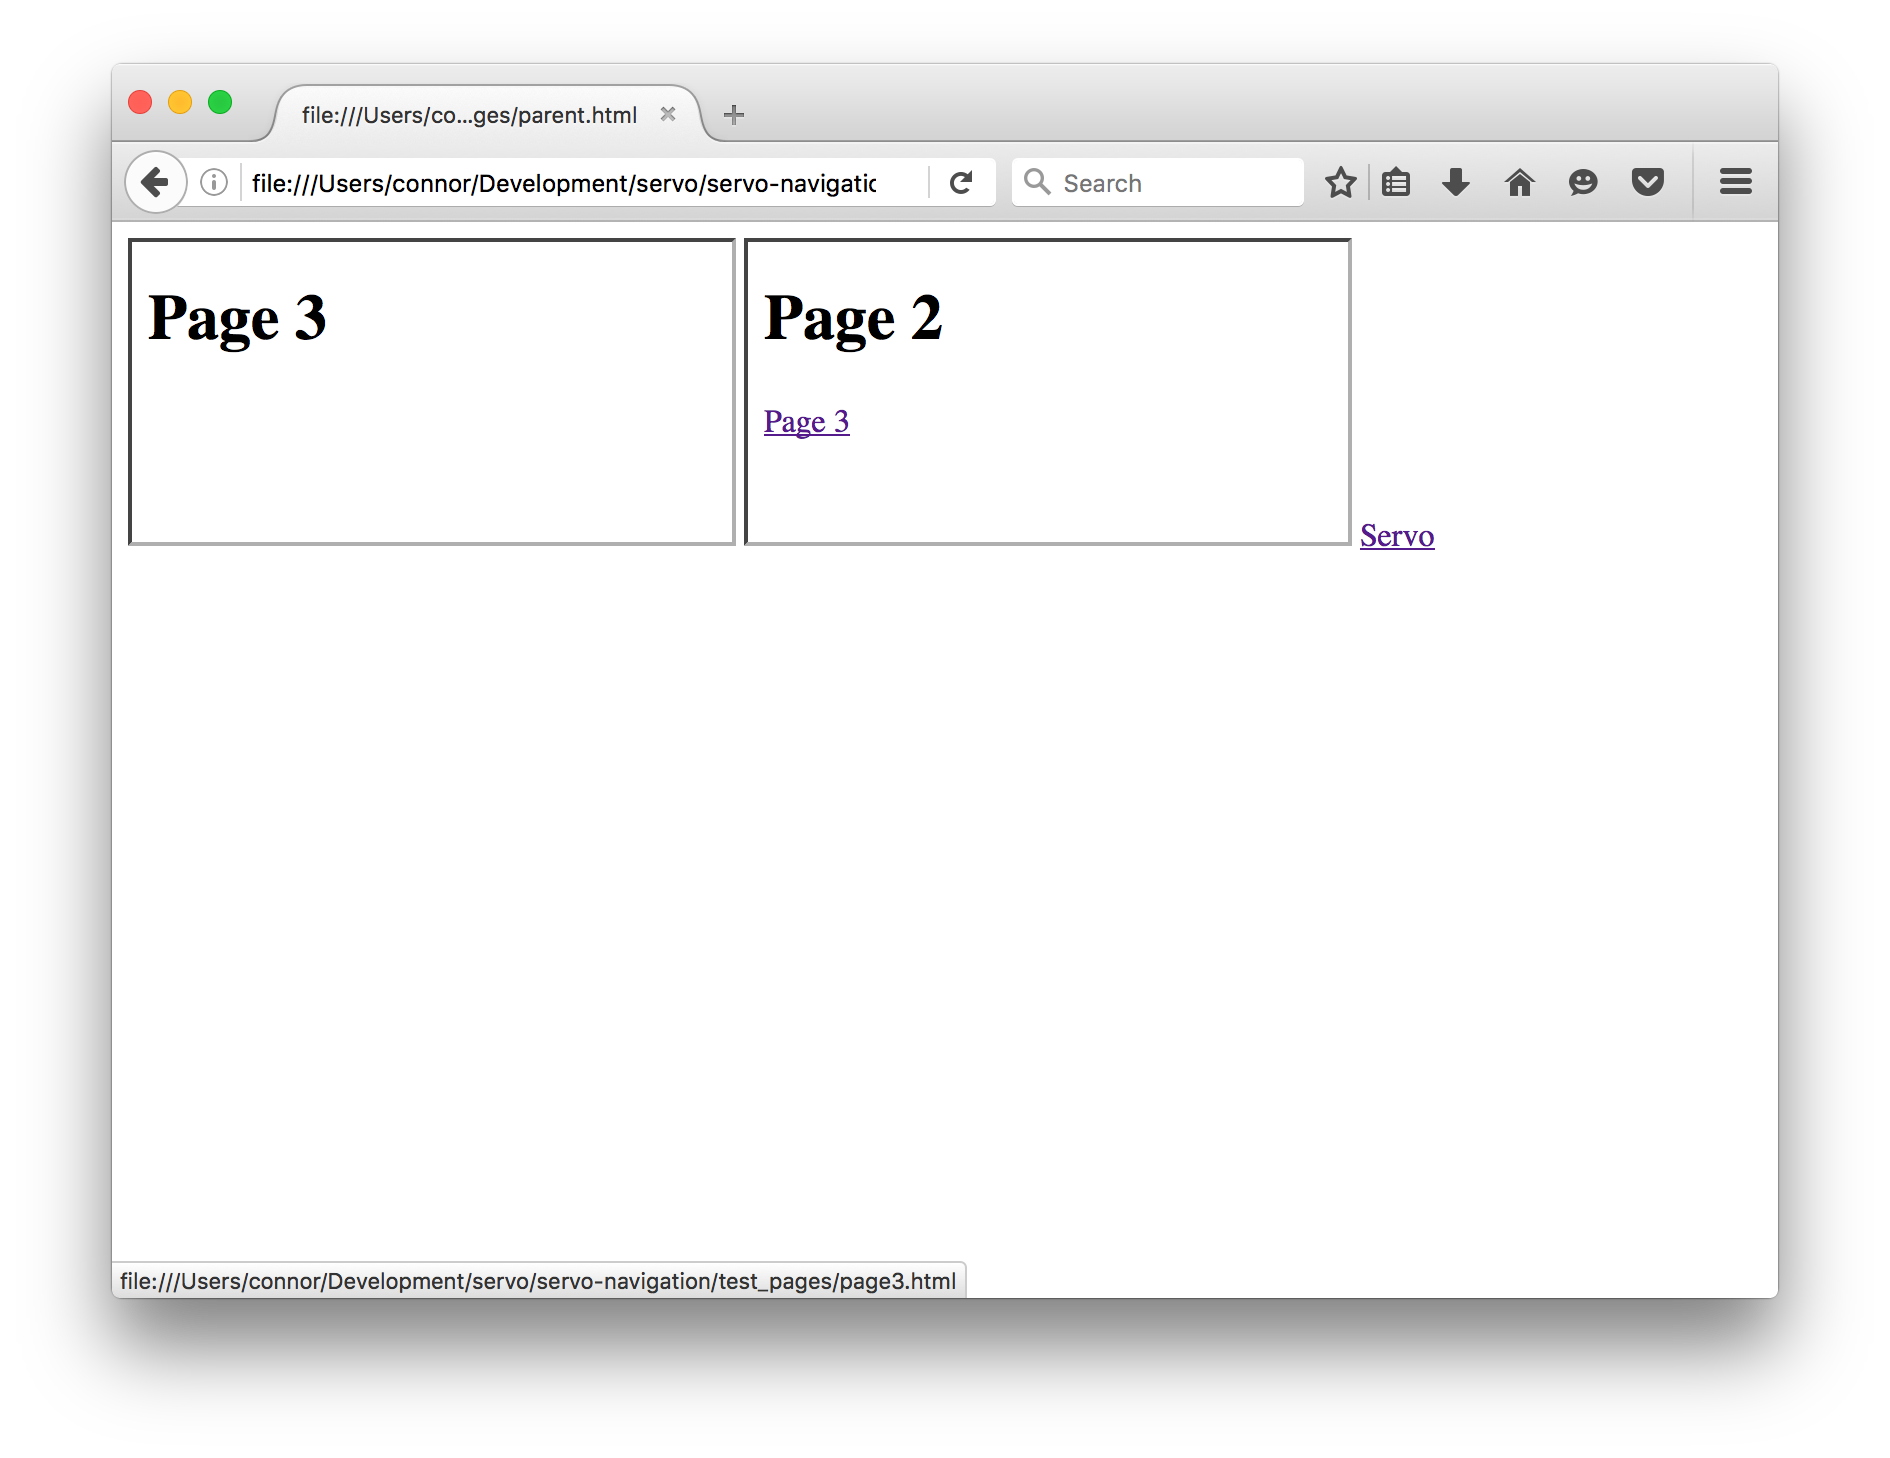
\includegraphics[width=.5\linewidth]{images/experiments/forwardback4/firefox/4.png}
    }~\raisebox{-.5\height}{
      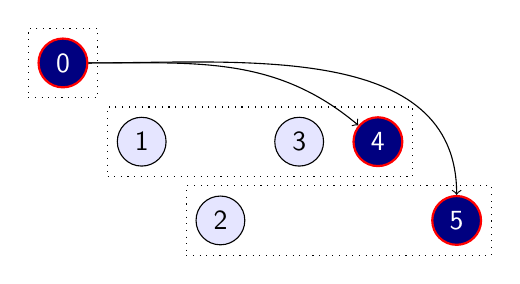
\begin{tikzpicture}
        \node[doc,active,fully](0) at (0,0){0};
        \node[doc](1) at (1,-1){1};
        \node[doc](2) at (2,-2){2};
        \node[doc](3) at (3,-1){3};
        \node[doc,active,fully](4) at (4,-1){4};
        \node[doc,jshactive,fully](5) at (5,-2){5};
        \node[draw,dotted,fit=(0)]{};
        \node[draw,dotted,fit=(1)(4)]{};
        \node[draw,dotted,fit=(2)(5)]{};
        \draw[->](0)to[out=0,in=140](4);
        \draw[->](0)to[out=0,in=90](5);
      \end{tikzpicture}
    }
    \caption{Navigate document $2$ to Page 2.}
  \end{figure}

  Navigate document $5$ to Page 3:
  \begin{figure}[H]
    \raisebox{-.5\height}{
      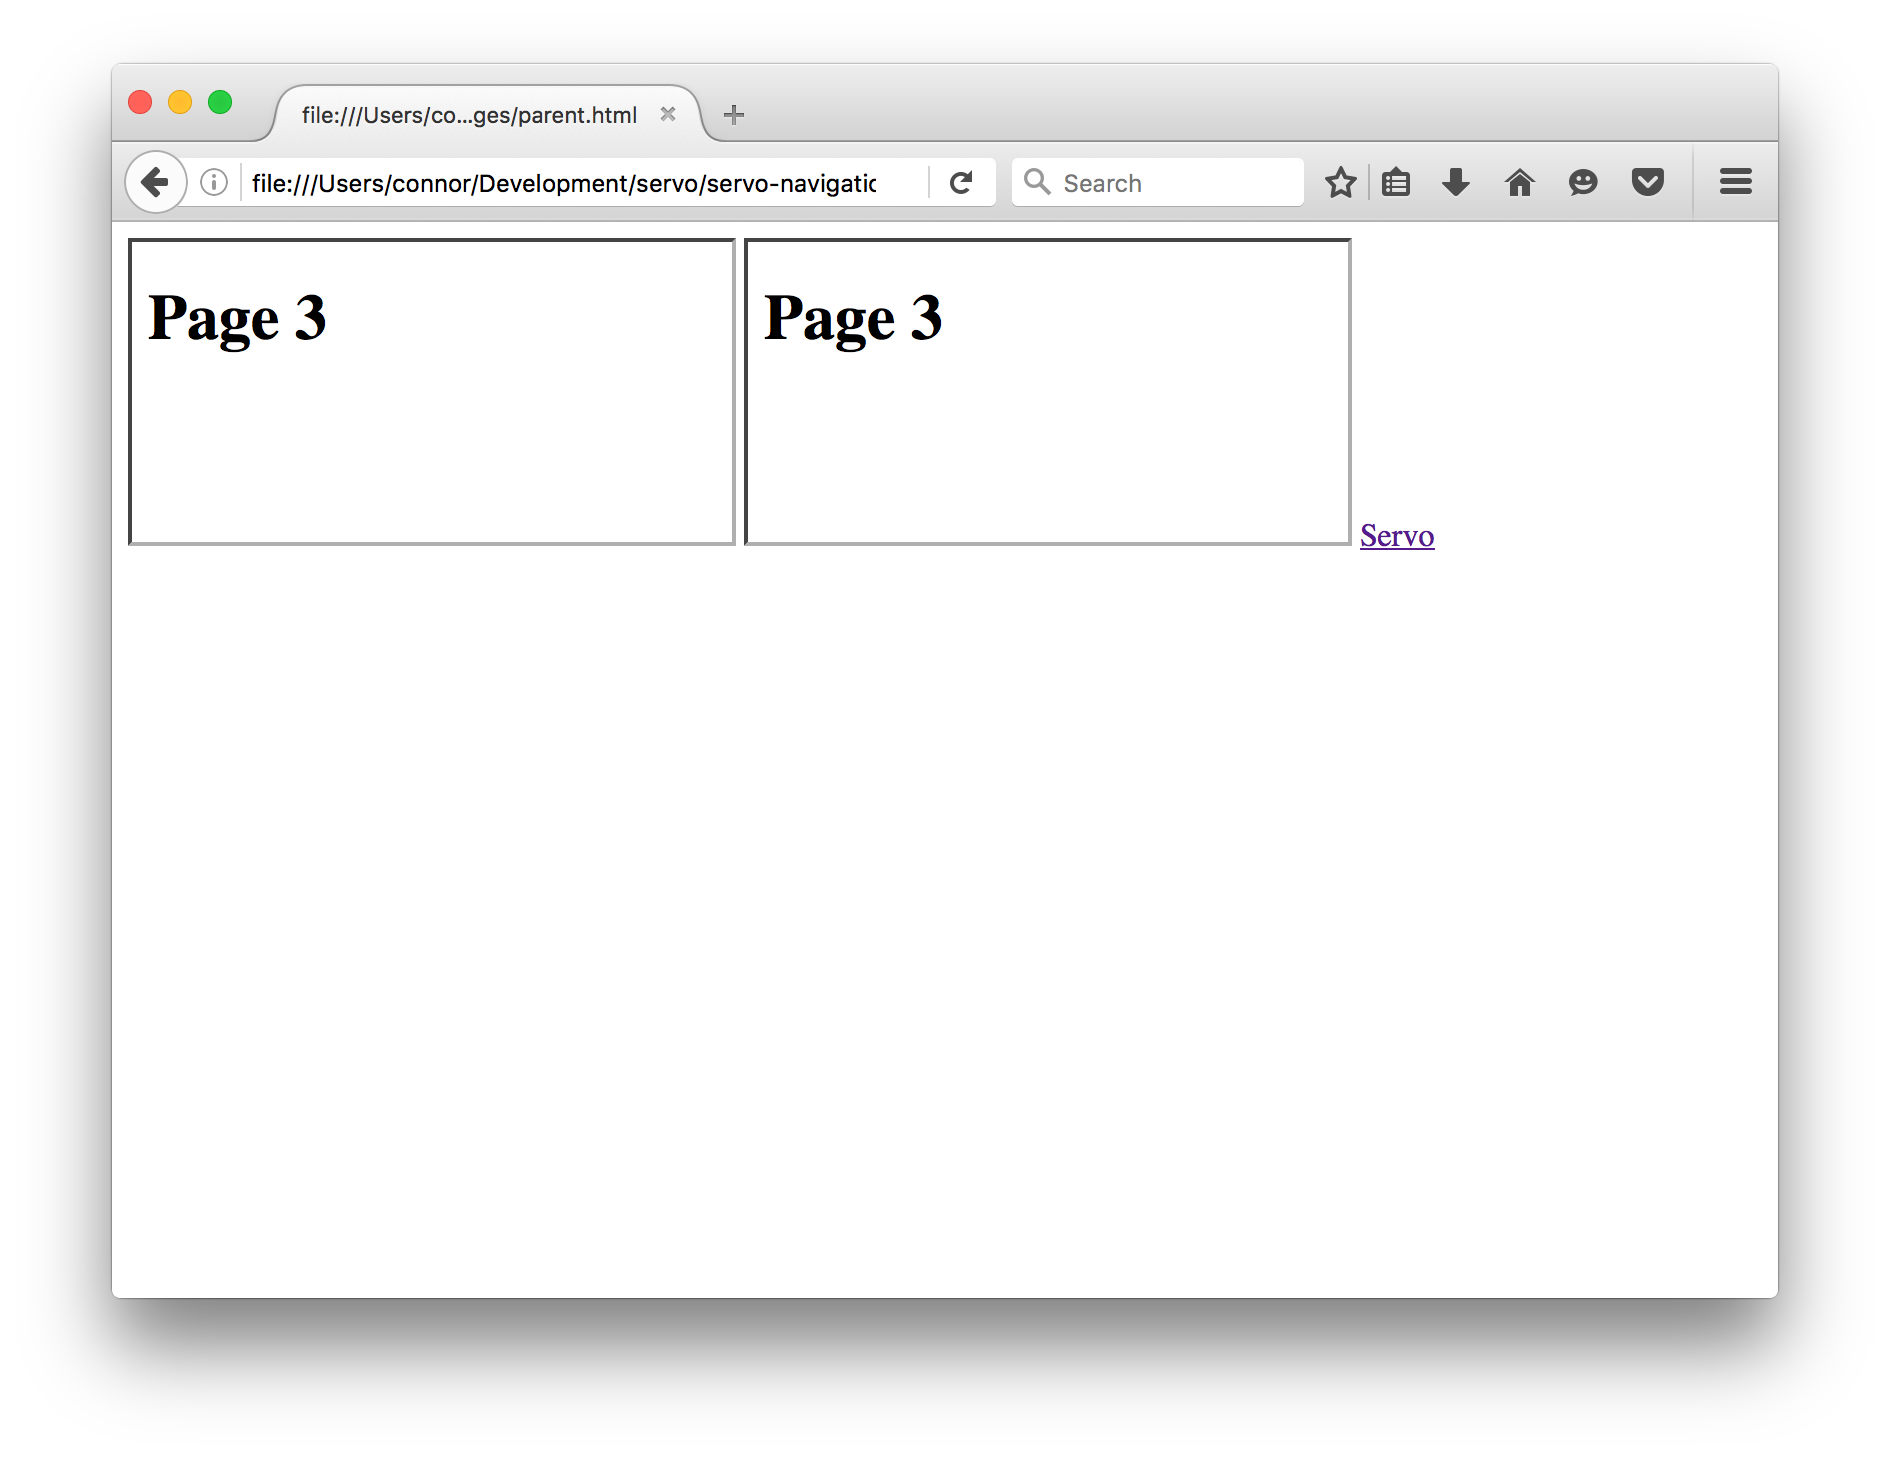
\includegraphics[width=.5\linewidth]{images/experiments/forwardback4/firefox/5.png}
    }~\raisebox{-.5\height}{
      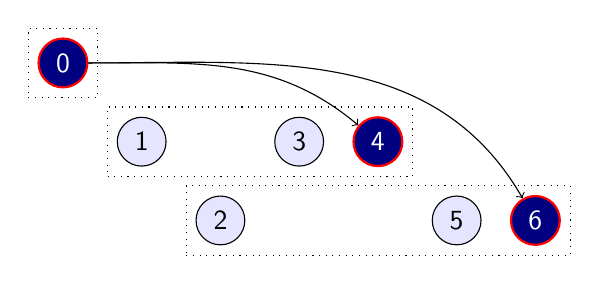
\begin{tikzpicture}
        \node[doc,active,fully](0) at (0,0){0};
        \node[doc](1) at (1,-1){1};
        \node[doc](2) at (2,-2){2};
        \node[doc](3) at (3,-1){3};
        \node[doc,active,fully](4) at (4,-1){4};
        \node[doc](5) at (5,-2){5};
        \node[doc,jshactive,fully](6) at (6,-2){6};
        \node[draw,dotted,fit=(0)]{};
        \node[draw,dotted,fit=(1)(4)]{};
        \node[draw,dotted,fit=(2)(6)]{};
        \draw[->](0)to[out=0,in=140](4);
        \draw[->](0)to[out=0,in=120](6);
      \end{tikzpicture}
    }
    \caption{Navigate document $5$ to Page 3.}
  \end{figure}

  \emph{$\aNH$ traverses the history by $-4$ to $\aNH'$}:
  \begin{figure}[H]
    \raisebox{-.5\height}{
      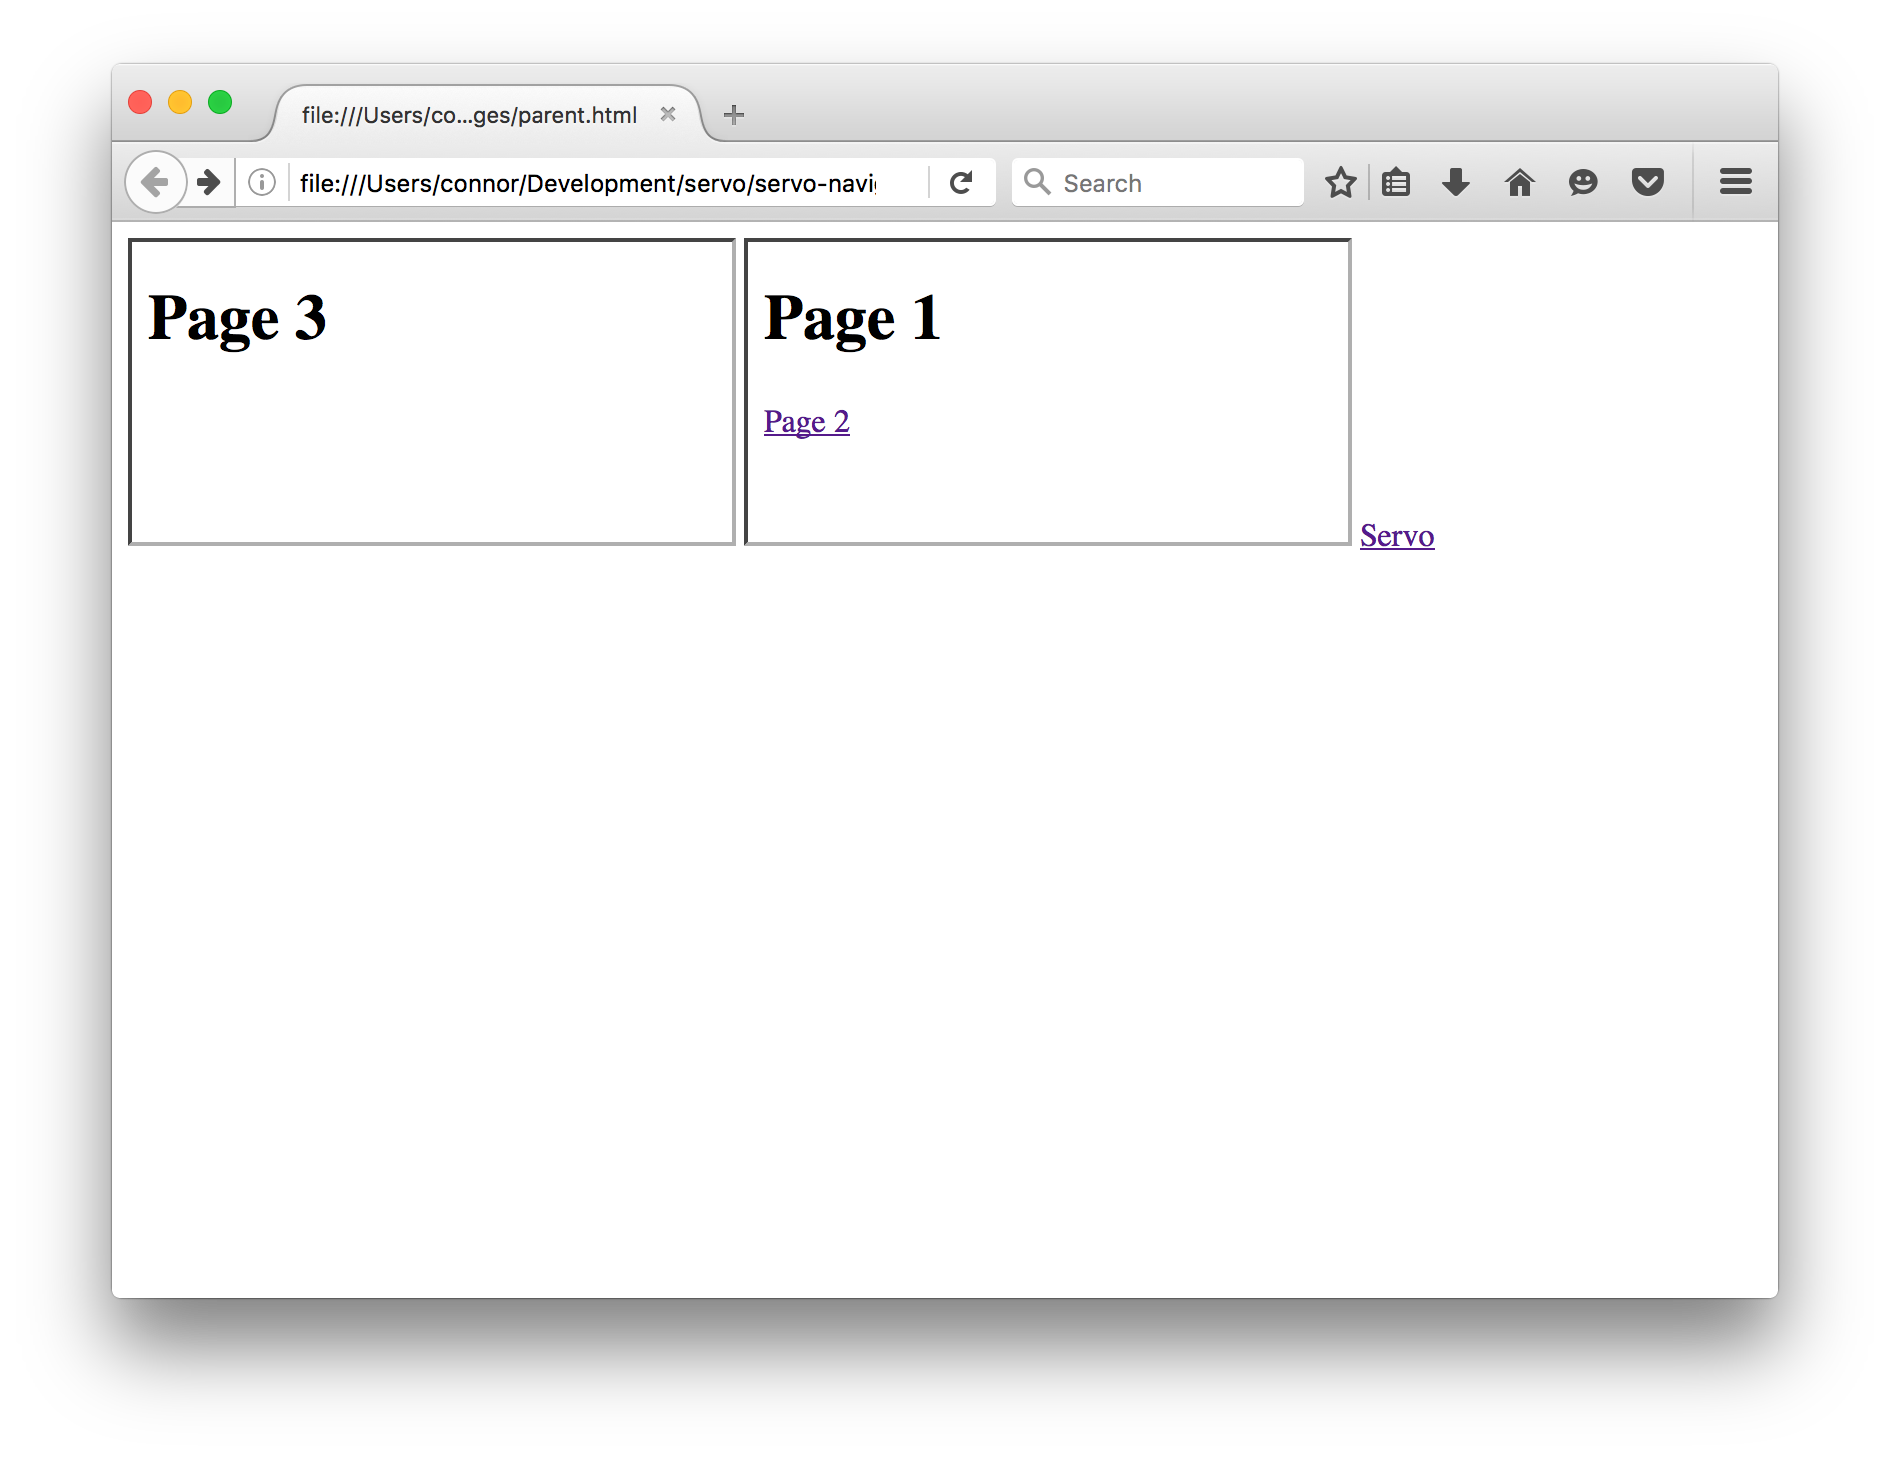
\includegraphics[width=.5\linewidth]{images/experiments/forwardback4/firefox/6.png}
    }~\raisebox{-.5\height}{
      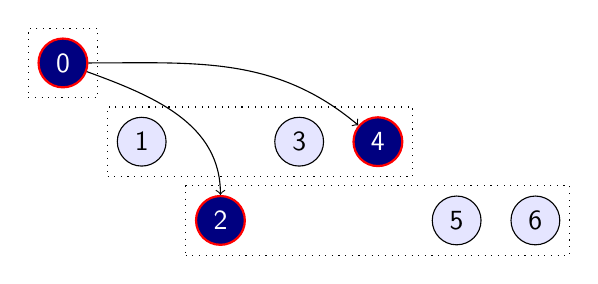
\begin{tikzpicture}
        \node[doc,active,fully](0) at (0,0){0};
        \node[doc](1) at (1,-1){1};
        \node[doc,jshactive,fully](2) at (2,-2){2};
        \node[doc](3) at (3,-1){3};
        \node[doc,active,fully](4) at (4,-1){4};
        \node[doc](5) at (5,-2){5};
        \node[doc](6) at (6,-2){6};
        \node[draw,dotted,fit=(0)]{};
        \node[draw,dotted,fit=(1)(4)]{};
        \node[draw,dotted,fit=(2)(6)]{};
        \draw[->](0)to[out=0,in=140](4);
        \draw[->](0)to[out=-20,in=90](2);
      \end{tikzpicture}
    }
    \caption{Traversal by $-4$.}
    \label{fig:traverseback4}
  \end{figure}

  This state is obviously wrong, as document $4$ should have traversed to document $1$.
  This is similar to counterexample~\ref{counterexample:homomorphism1}.

  \emph{$\aNH'$ traverses the history by $4$ to $\aNH''$}:
  \begin{figure}[H]
    \raisebox{-.5\height}{
      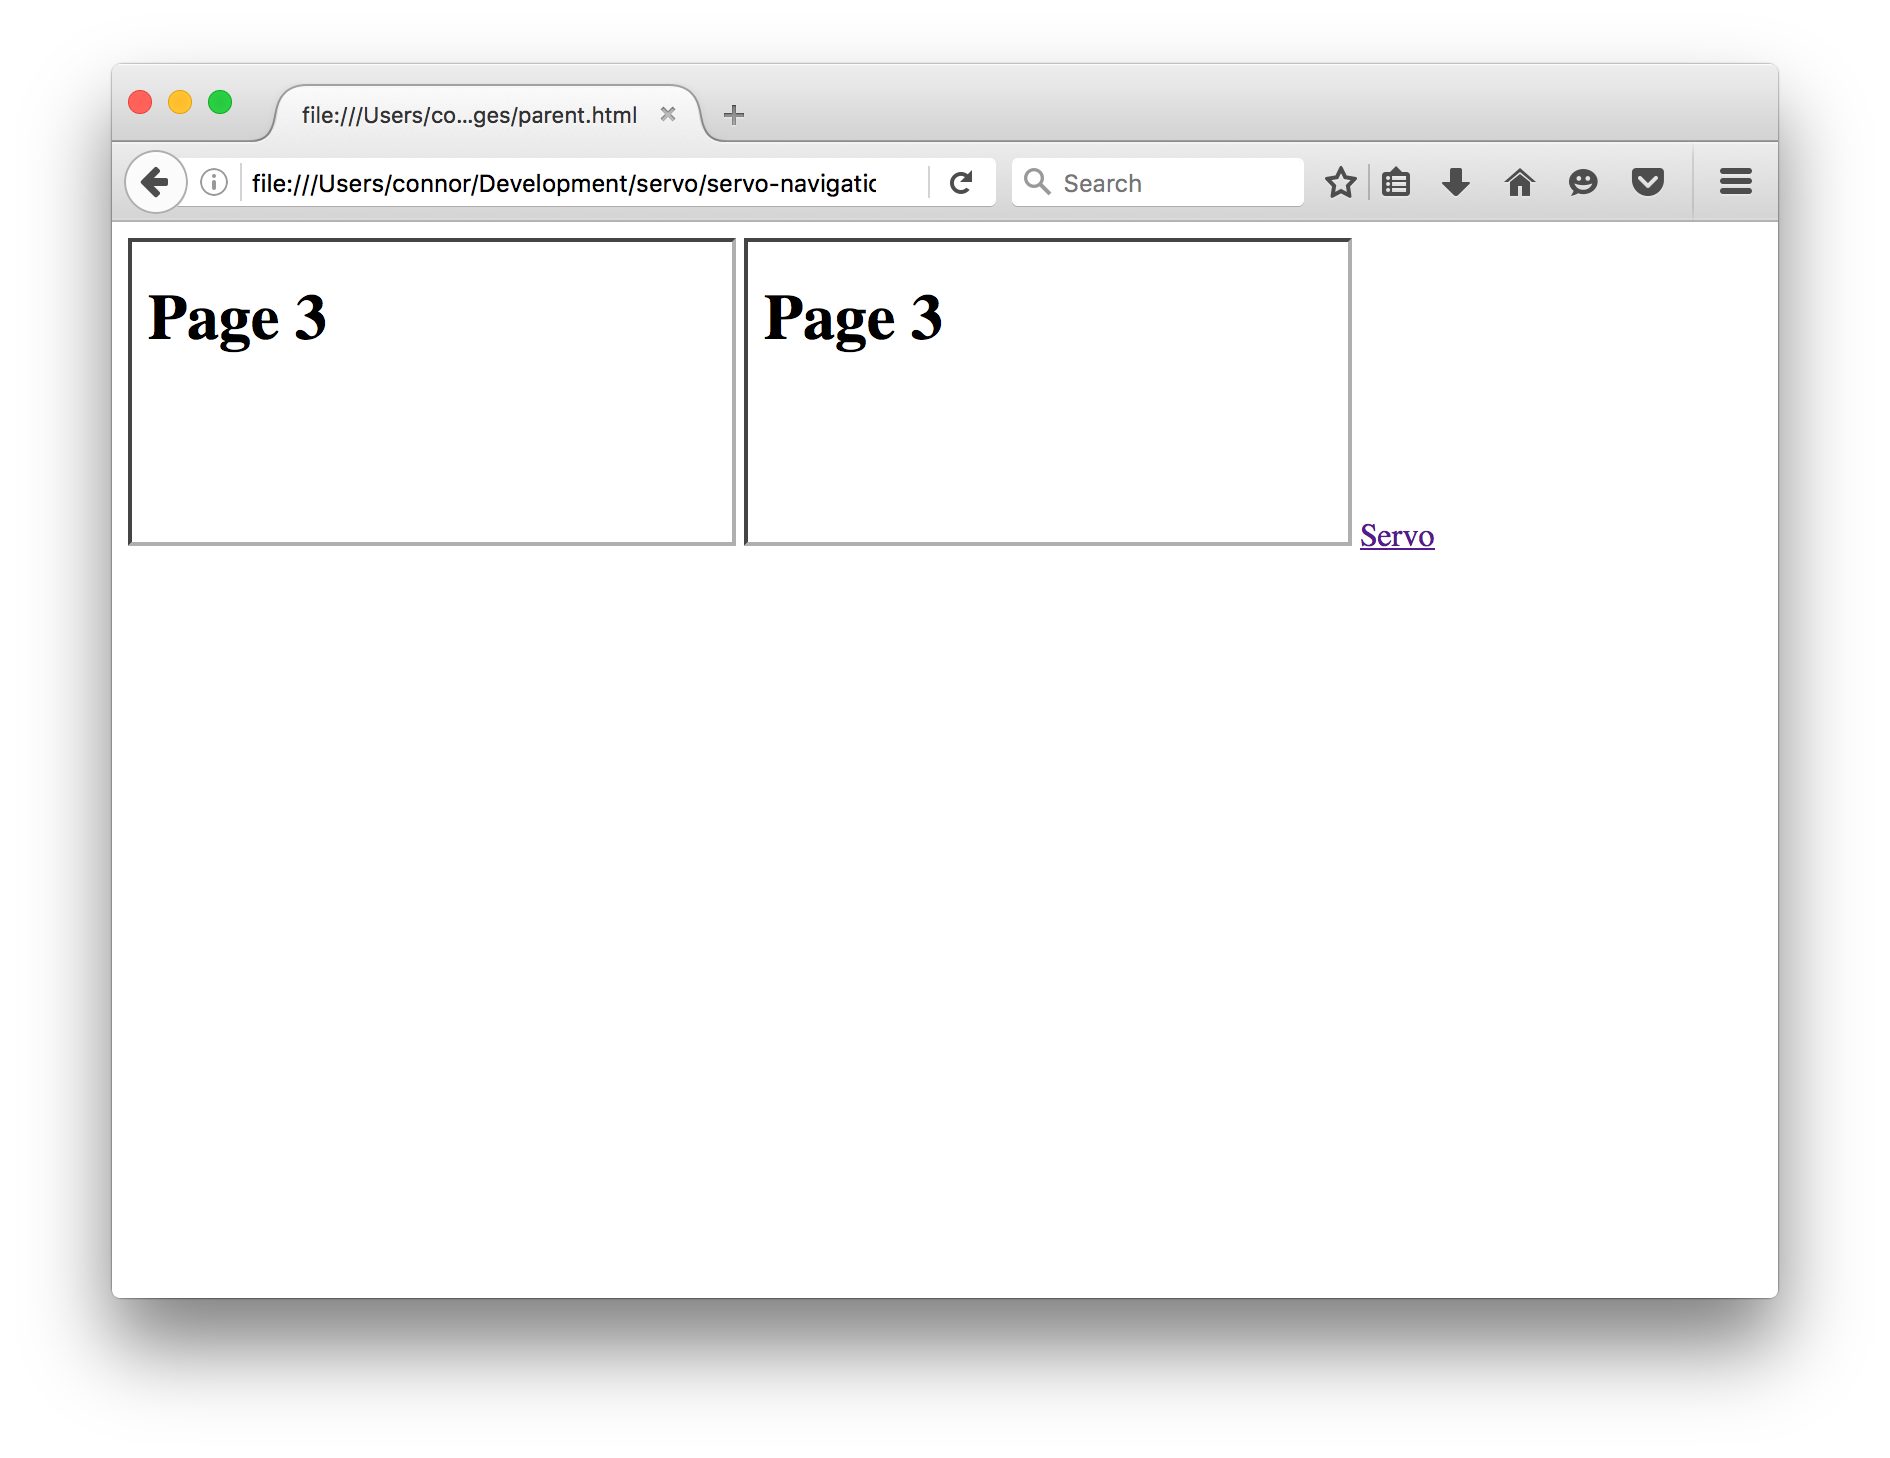
\includegraphics[width=.5\linewidth]{images/experiments/forwardback4/firefox/7.png}
    }~\raisebox{-.5\height}{
      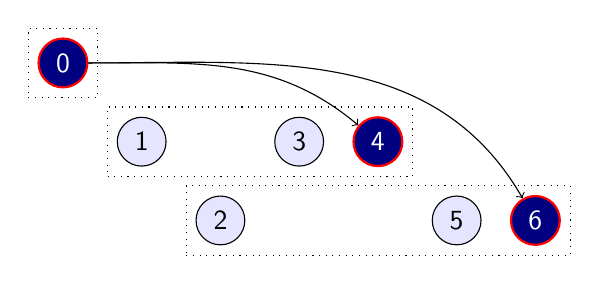
\begin{tikzpicture}
        \node[doc,active,fully](0) at (0,0){0};
        \node[doc](1) at (1,-1){1};
        \node[doc](2) at (2,-2){2};
        \node[doc](3) at (3,-1){3};
        \node[doc,active,fully](4) at (4,-1){4};
        \node[doc](5) at (5,-2){5};
        \node[doc,jshactive,fully](6) at (6,-2){6};
        \node[draw,dotted,fit=(0)]{};
        \node[draw,dotted,fit=(1)(4)]{};
        \node[draw,dotted,fit=(2)(6)]{};
        \draw[->](0)to[out=0,in=140](4);
        \draw[->](0)to[out=0,in=120](6);
      \end{tikzpicture}
    }
    \caption{Traversal by $4$.}
  \end{figure}

  While this result does satisfy Goal~\ref{goal:homomorphism}, there are still some issues:
  \begin{itemize}
    \item Figure~\ref{fig:traverseback4} yields an incorrect traversal. [CGB: I believe this actually does break Goal~\ref{goal:homomorphism} as navigating by $-1$ four times should yield the correct state.]
    \item It is impossible to get back to Page 1 on both Frames. [CGB: Looks to be a bug in FF, when holding down the back button, the list of pages to traverse to shows up. Clicking on the oldest item on the list does nothing and does not activate that item.]
  \end{itemize}

  Safari:
  \begin{figure}[H]
    \raisebox{-.5\height}{
      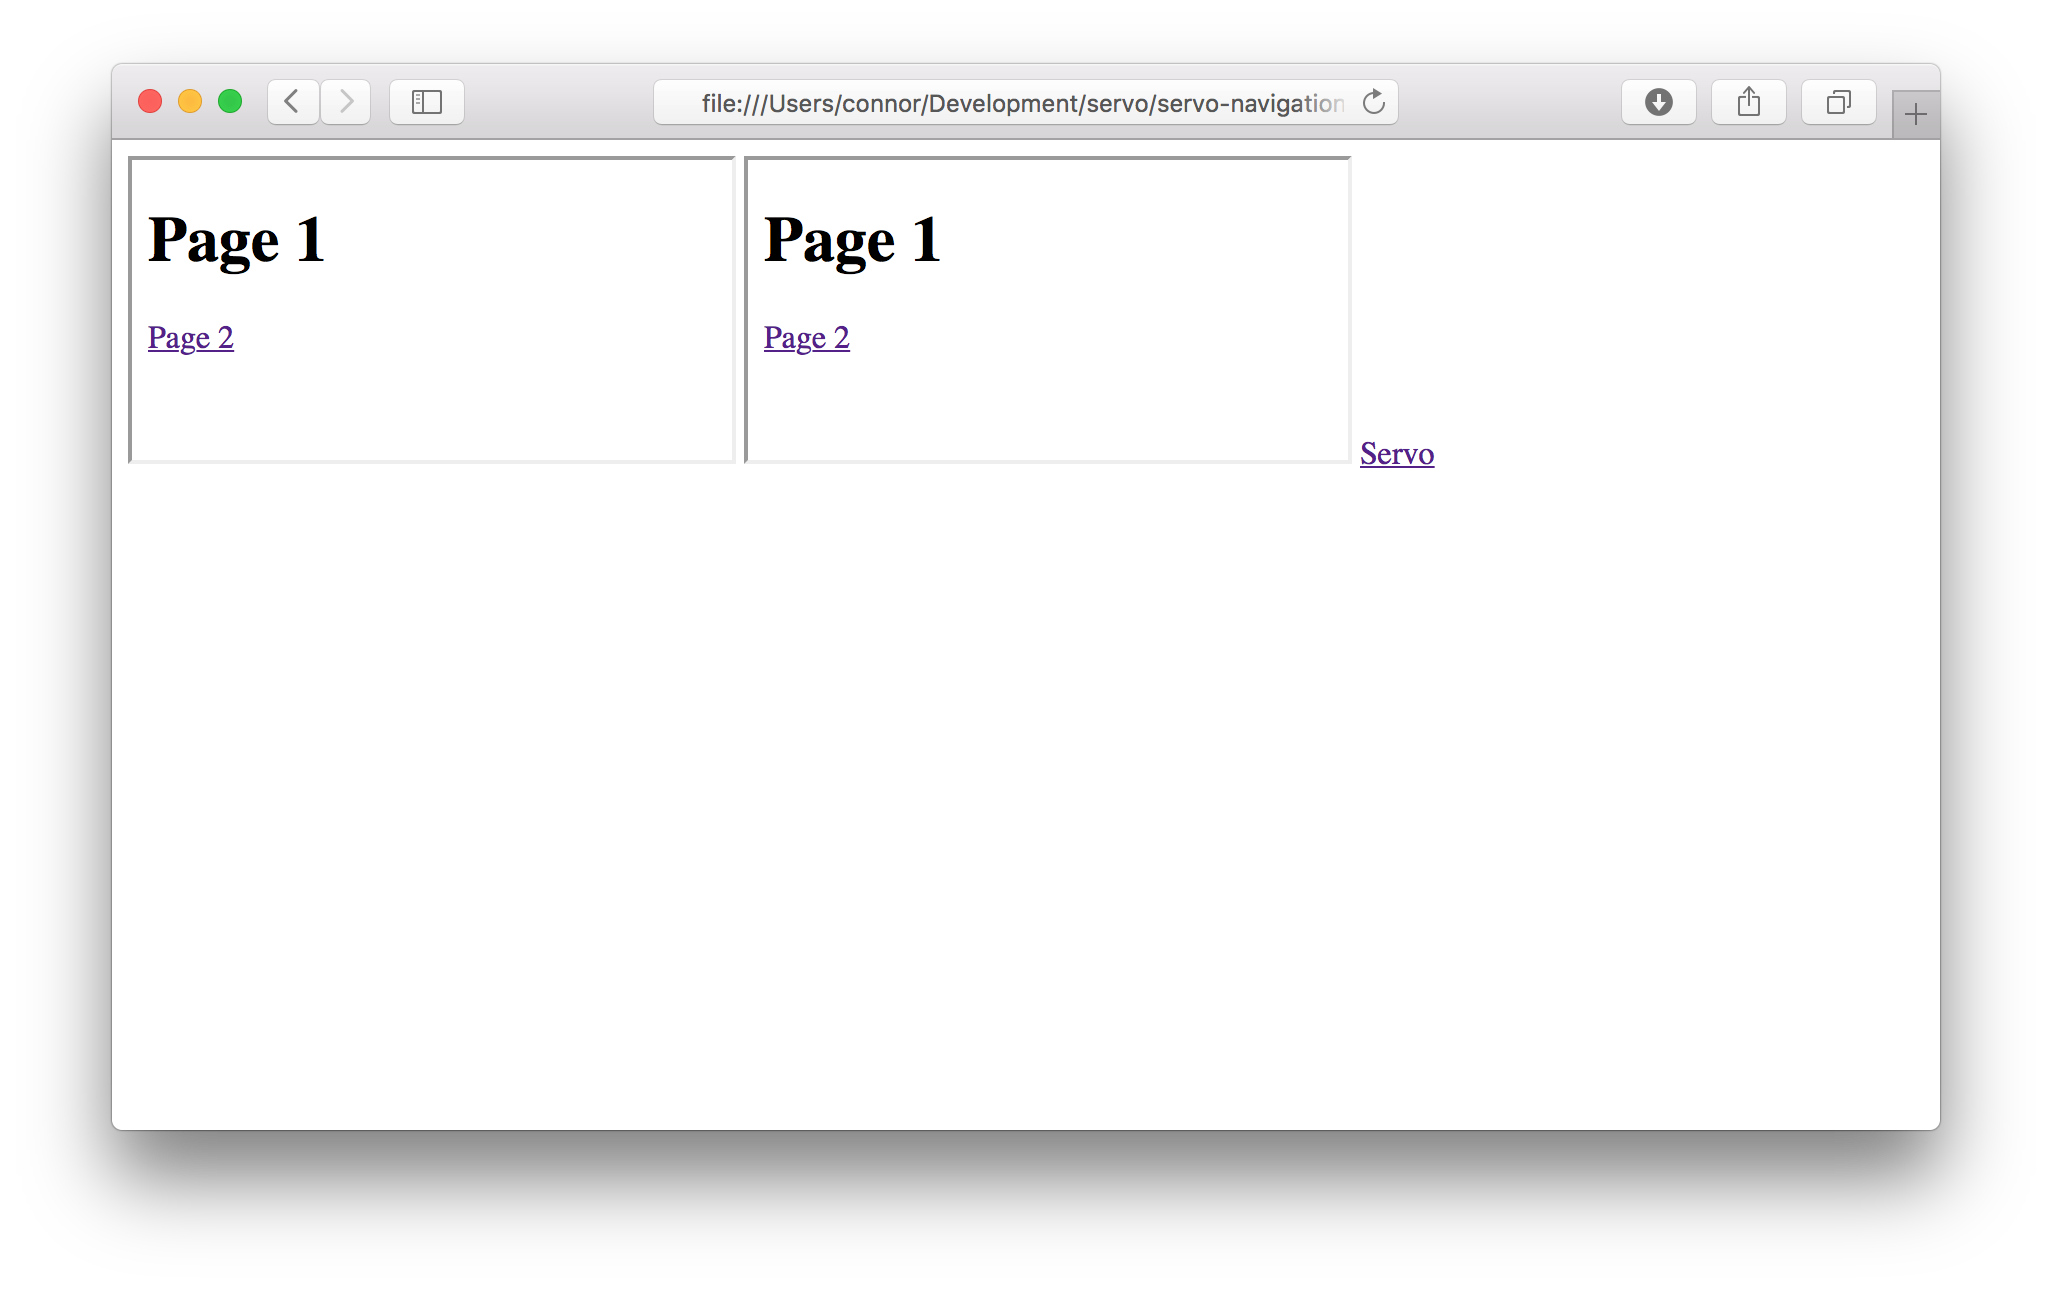
\includegraphics[width=.5\linewidth]{images/experiments/forwardback4/safari/1.png}%
    }~\raisebox{-.5\height}{
      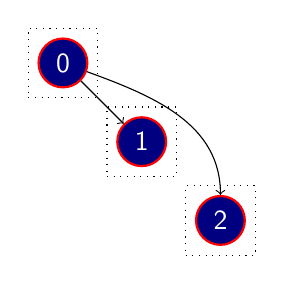
\begin{tikzpicture}
        \node[doc,active,fully](0) at (0,0){0};
        \node[doc,active,fully](1) at (1,-1){1};
        \node[doc,jshactive,fully](2) at (2,-2){2};
        \node[draw,dotted,fit=(0)]{};
        \node[draw,dotted,fit=(1)]{};
        \node[draw,dotted,fit=(2)]{};
        \draw[->](0)--(1);
        \draw[->](0)to[out=-20,in=90](2);
      \end{tikzpicture}
    }
    \caption{Initial State}
  \end{figure}

  Navigate document $1$ to Page 2:
  \begin{figure}[H]
    \raisebox{-.5\height}{
      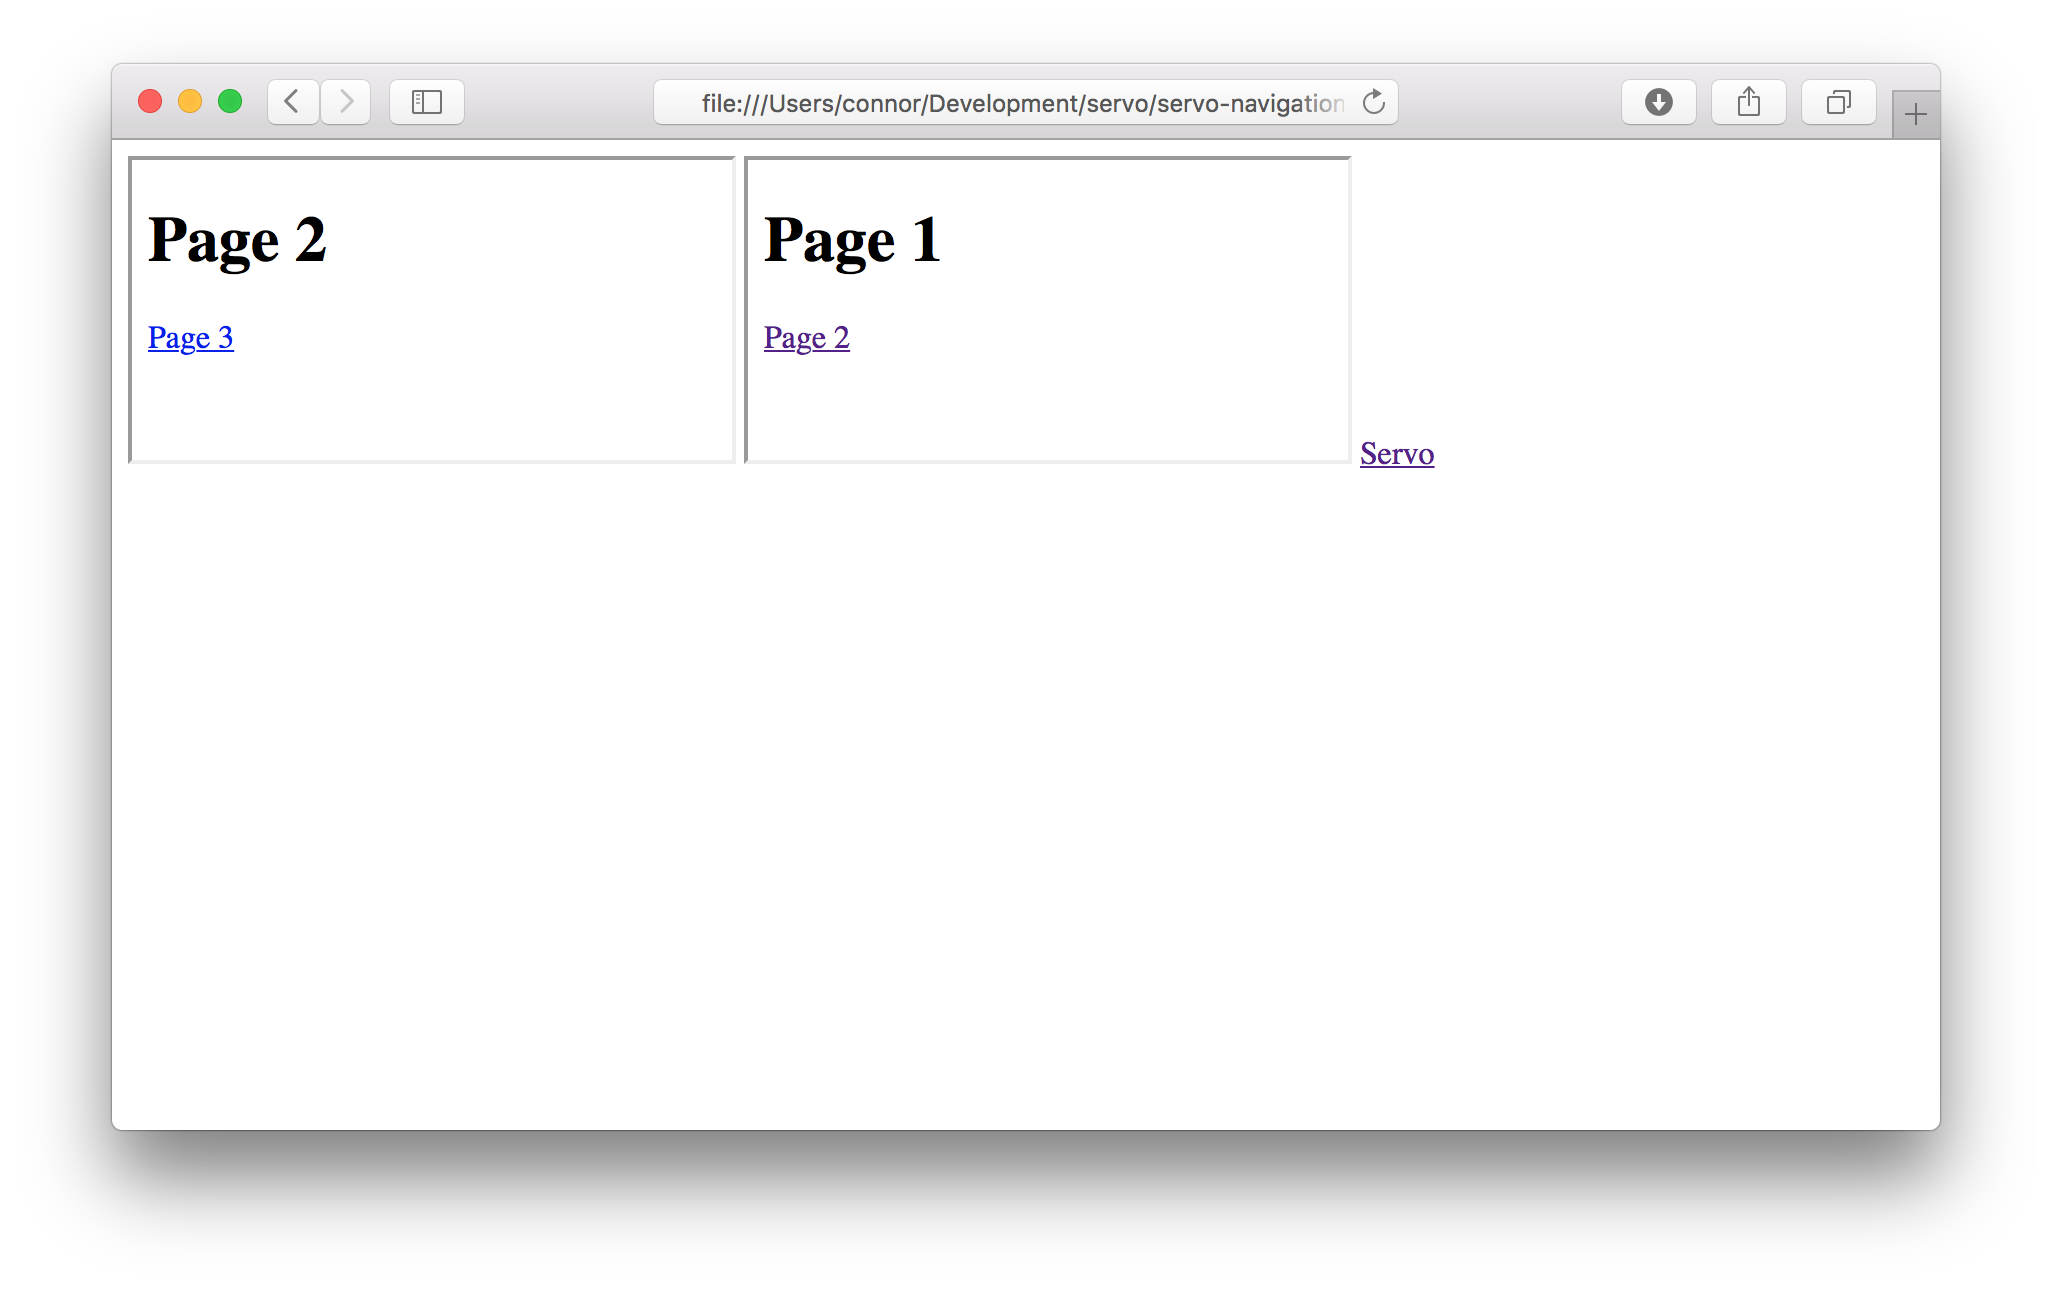
\includegraphics[width=.5\linewidth]{images/experiments/forwardback4/safari/2.png}
    }~\raisebox{-.5\height}{
      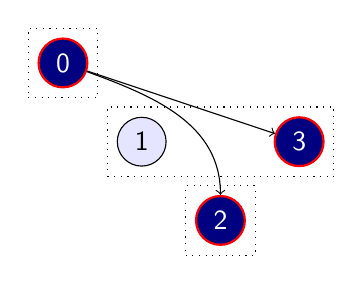
\begin{tikzpicture}
        \node[doc,active,fully](0) at (0,0){0};
        \node[doc](1) at (1,-1){1};
        \node[doc,active,fully](2) at (2,-2){2};
        \node[doc,jshactive,fully](3) at (3,-1){3};
        \node[draw,dotted,fit=(0)]{};
        \node[draw,dotted,fit=(1)(3)]{};
        \node[draw,dotted,fit=(2)]{};
        \draw[->](0)--(3);
        \draw[->](0)to[out=-20,in=90](2);
      \end{tikzpicture}
    }
    \caption{Navigate document $1$ to Page 2.}
  \end{figure}

  Navigate document $3$ to Page 3:
  \begin{figure}[H]
    \raisebox{-.5\height}{
      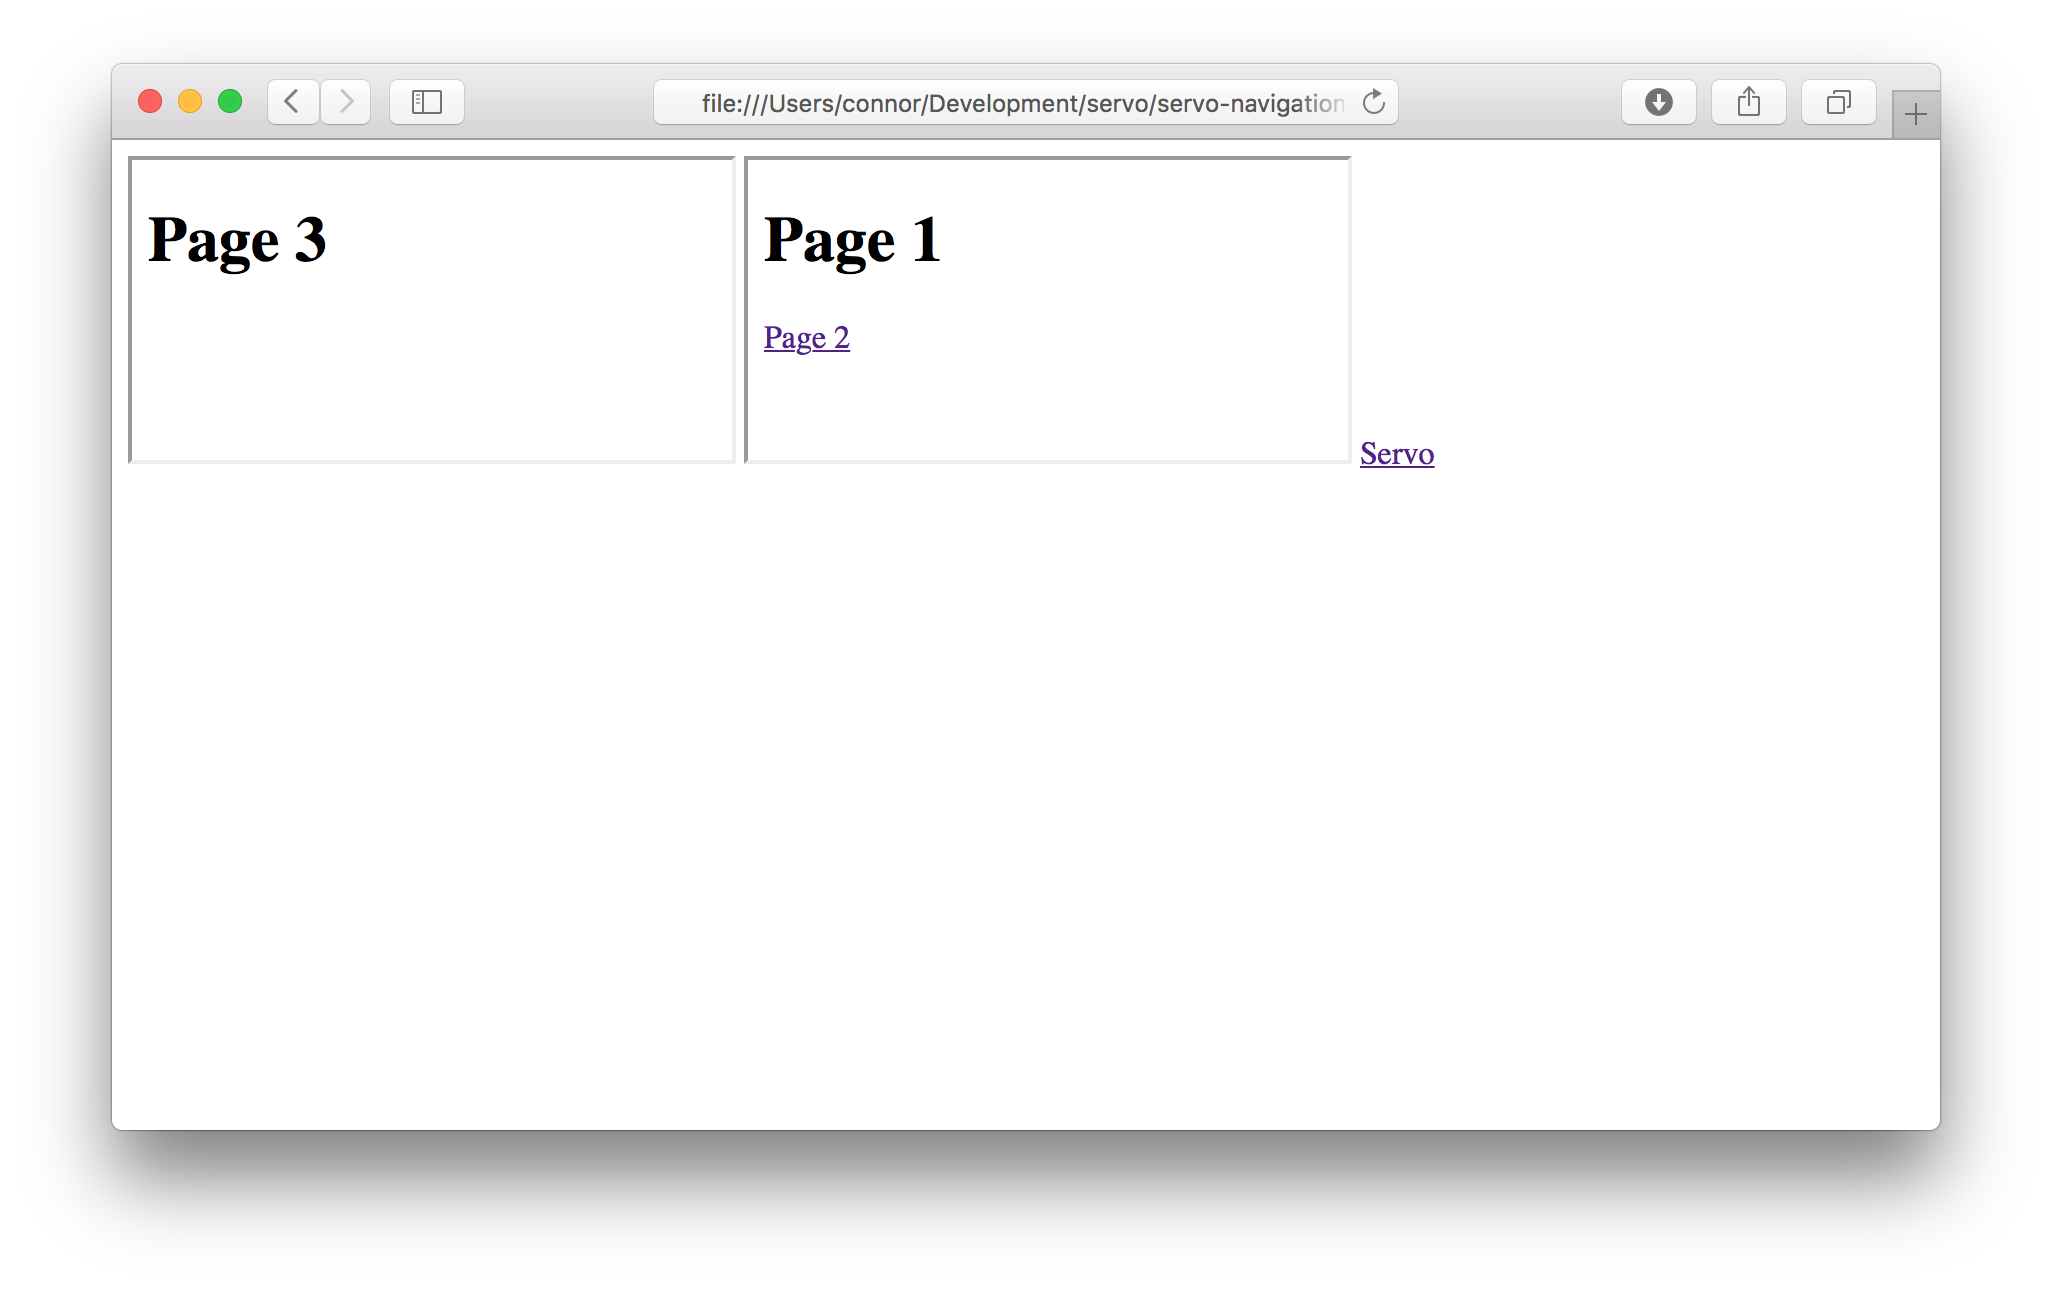
\includegraphics[width=.5\linewidth]{images/experiments/forwardback4/safari/3.png}
    }~\raisebox{-.5\height}{
      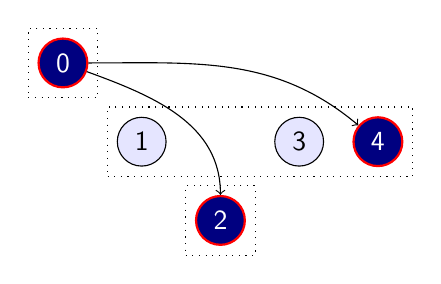
\begin{tikzpicture}
        \node[doc,active,fully](0) at (0,0){0};
        \node[doc](1) at (1,-1){1};
        \node[doc,active,fully](2) at (2,-2){2};
        \node[doc](3) at (3,-1){3};
        \node[doc,jshactive,fully](4) at (4,-1){4};
        \node[draw,dotted,fit=(0)]{};
        \node[draw,dotted,fit=(1)(4)]{};
        \node[draw,dotted,fit=(2)]{};
        \draw[->](0)to[out=0,in=140](4);
        \draw[->](0)to[out=-20,in=90](2);
      \end{tikzpicture}
    }
    \caption{Navigate document $3$ to Page 3.}
  \end{figure}

  Navigate document $2$ to Page 2:
  \begin{figure}[H]
    \raisebox{-.5\height}{
      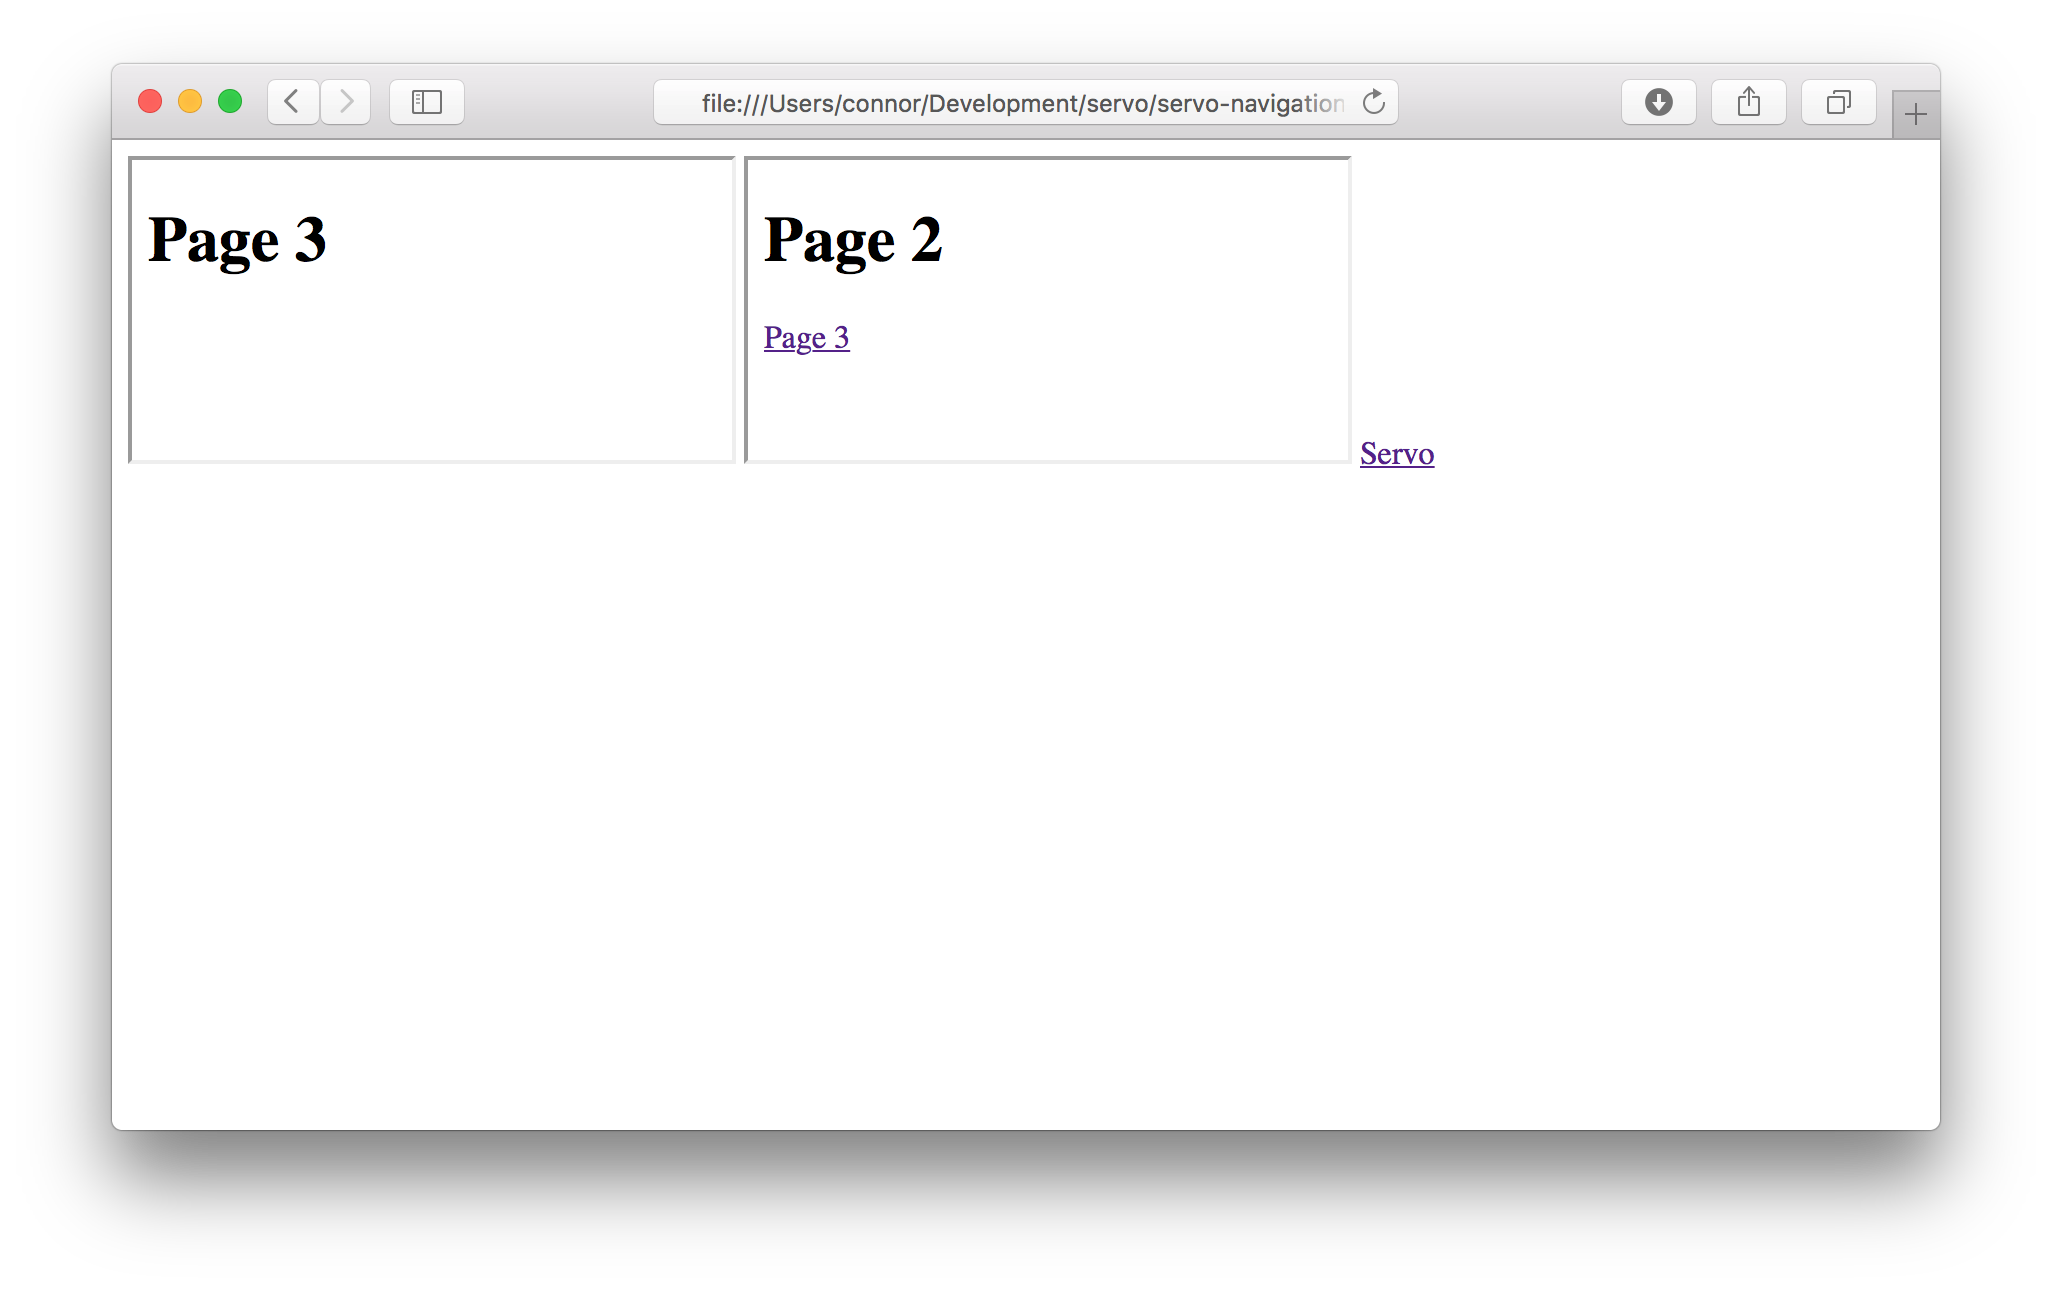
\includegraphics[width=.5\linewidth]{images/experiments/forwardback4/safari/4.png}
    }~\raisebox{-.5\height}{
      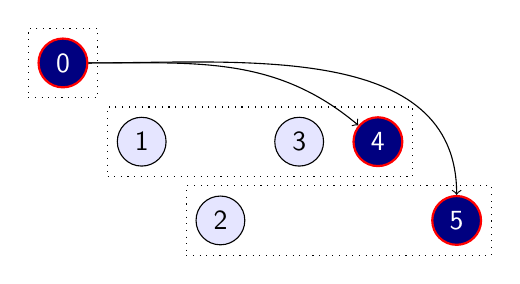
\begin{tikzpicture}
        \node[doc,active,fully](0) at (0,0){0};
        \node[doc](1) at (1,-1){1};
        \node[doc](2) at (2,-2){2};
        \node[doc](3) at (3,-1){3};
        \node[doc,active,fully](4) at (4,-1){4};
        \node[doc,jshactive,fully](5) at (5,-2){5};
        \node[draw,dotted,fit=(0)]{};
        \node[draw,dotted,fit=(1)(4)]{};
        \node[draw,dotted,fit=(2)(5)]{};
        \draw[->](0)to[out=0,in=140](4);
        \draw[->](0)to[out=0,in=90](5);
      \end{tikzpicture}
    }
    \caption{Navigate document $2$ to Page 2.}
  \end{figure}

  Navigate document $5$ to Page 3:
  \begin{figure}[H]
    \raisebox{-.5\height}{
      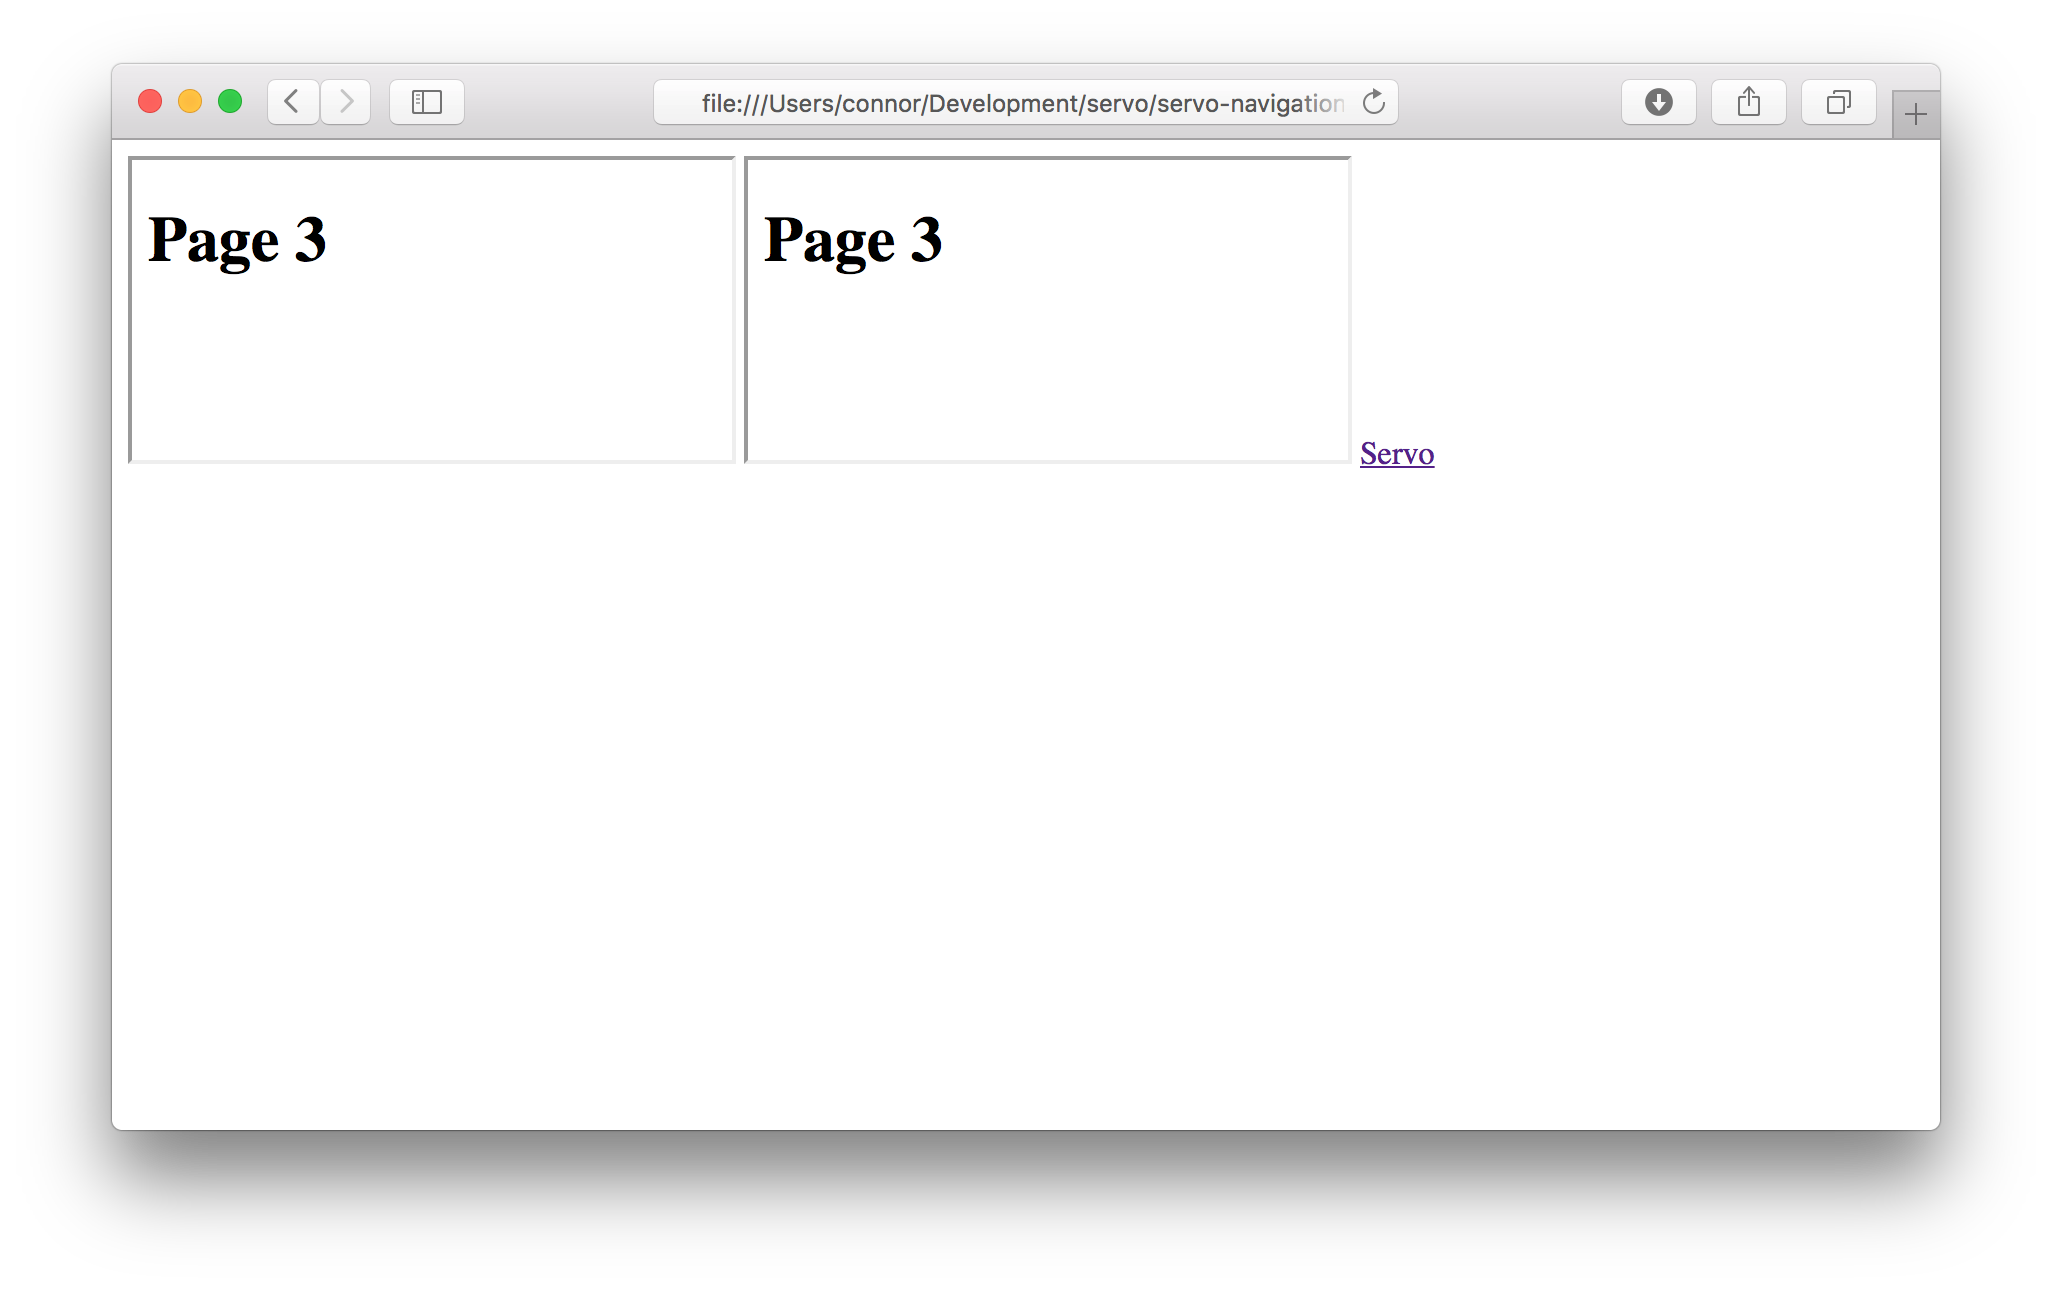
\includegraphics[width=.5\linewidth]{images/experiments/forwardback4/safari/5.png}
    }~\raisebox{-.5\height}{
      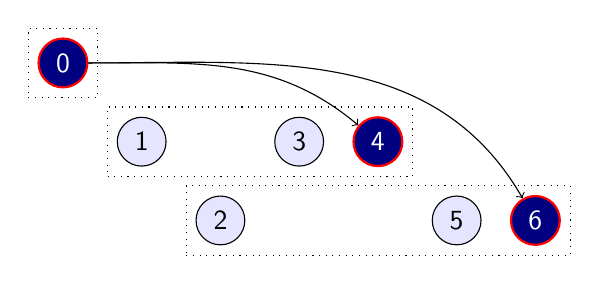
\begin{tikzpicture}
        \node[doc,active,fully](0) at (0,0){0};
        \node[doc](1) at (1,-1){1};
        \node[doc](2) at (2,-2){2};
        \node[doc](3) at (3,-1){3};
        \node[doc,active,fully](4) at (4,-1){4};
        \node[doc](5) at (5,-2){5};
        \node[doc,jshactive,fully](6) at (6,-2){6};
        \node[draw,dotted,fit=(0)]{};
        \node[draw,dotted,fit=(1)(4)]{};
        \node[draw,dotted,fit=(2)(6)]{};
        \draw[->](0)to[out=0,in=140](4);
        \draw[->](0)to[out=0,in=120](6);
      \end{tikzpicture}
    }
    \caption{Navigate document $5$ to Page 3.}
  \end{figure}

  \emph{$\aNH$ traverses the history by $-4$ to $\aNH'$}:
  \begin{figure}[H]
    \raisebox{-.5\height}{
      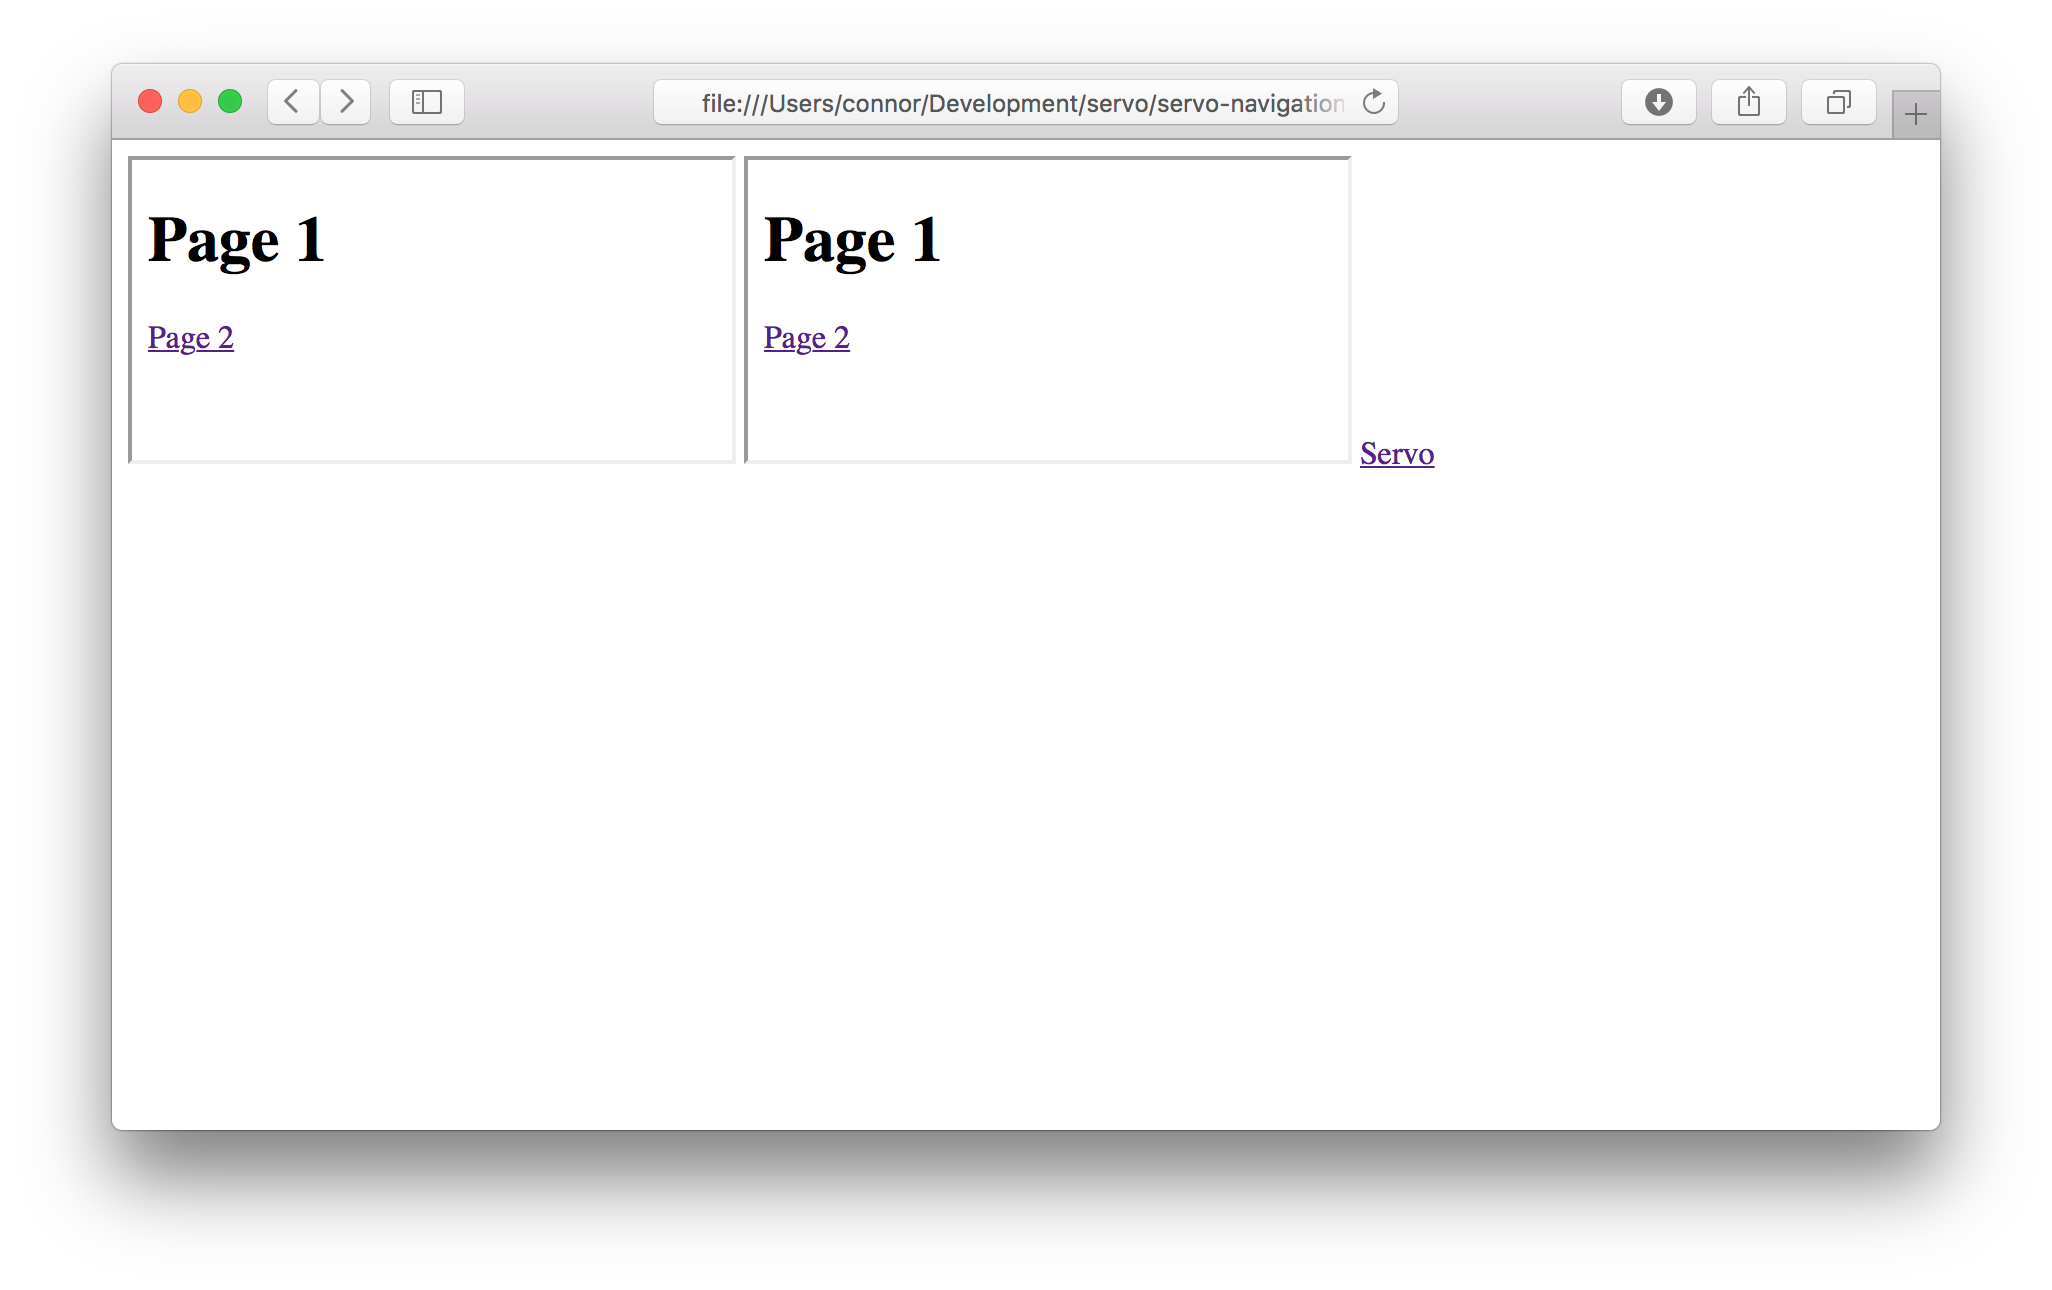
\includegraphics[width=.5\linewidth]{images/experiments/forwardback4/safari/6.png}
    }~\raisebox{-.5\height}{
      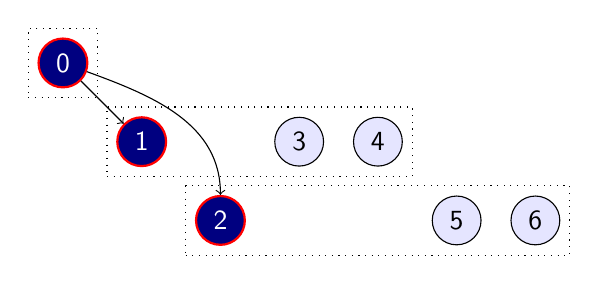
\begin{tikzpicture}
        \node[doc,active,fully](0) at (0,0){0};
        \node[doc,active,fully](1) at (1,-1){1};
        \node[doc,jshactive,fully](2) at (2,-2){2};
        \node[doc](3) at (3,-1){3};
        \node[doc](4) at (4,-1){4};
        \node[doc](5) at (5,-2){5};
        \node[doc](6) at (6,-2){6};
        \node[draw,dotted,fit=(0)]{};
        \node[draw,dotted,fit=(1)(4)]{};
        \node[draw,dotted,fit=(2)(6)]{};
        \draw[->](0)--(1);
        \draw[->](0)to[out=-20,in=90](2);
      \end{tikzpicture}
    }
    \caption{Traversal by $-4$.}
  \end{figure}

  \emph{$\aNH'$ traverses the history by $4$ to $\aNH''$}:
  \begin{figure}[H]
    \raisebox{-.5\height}{
      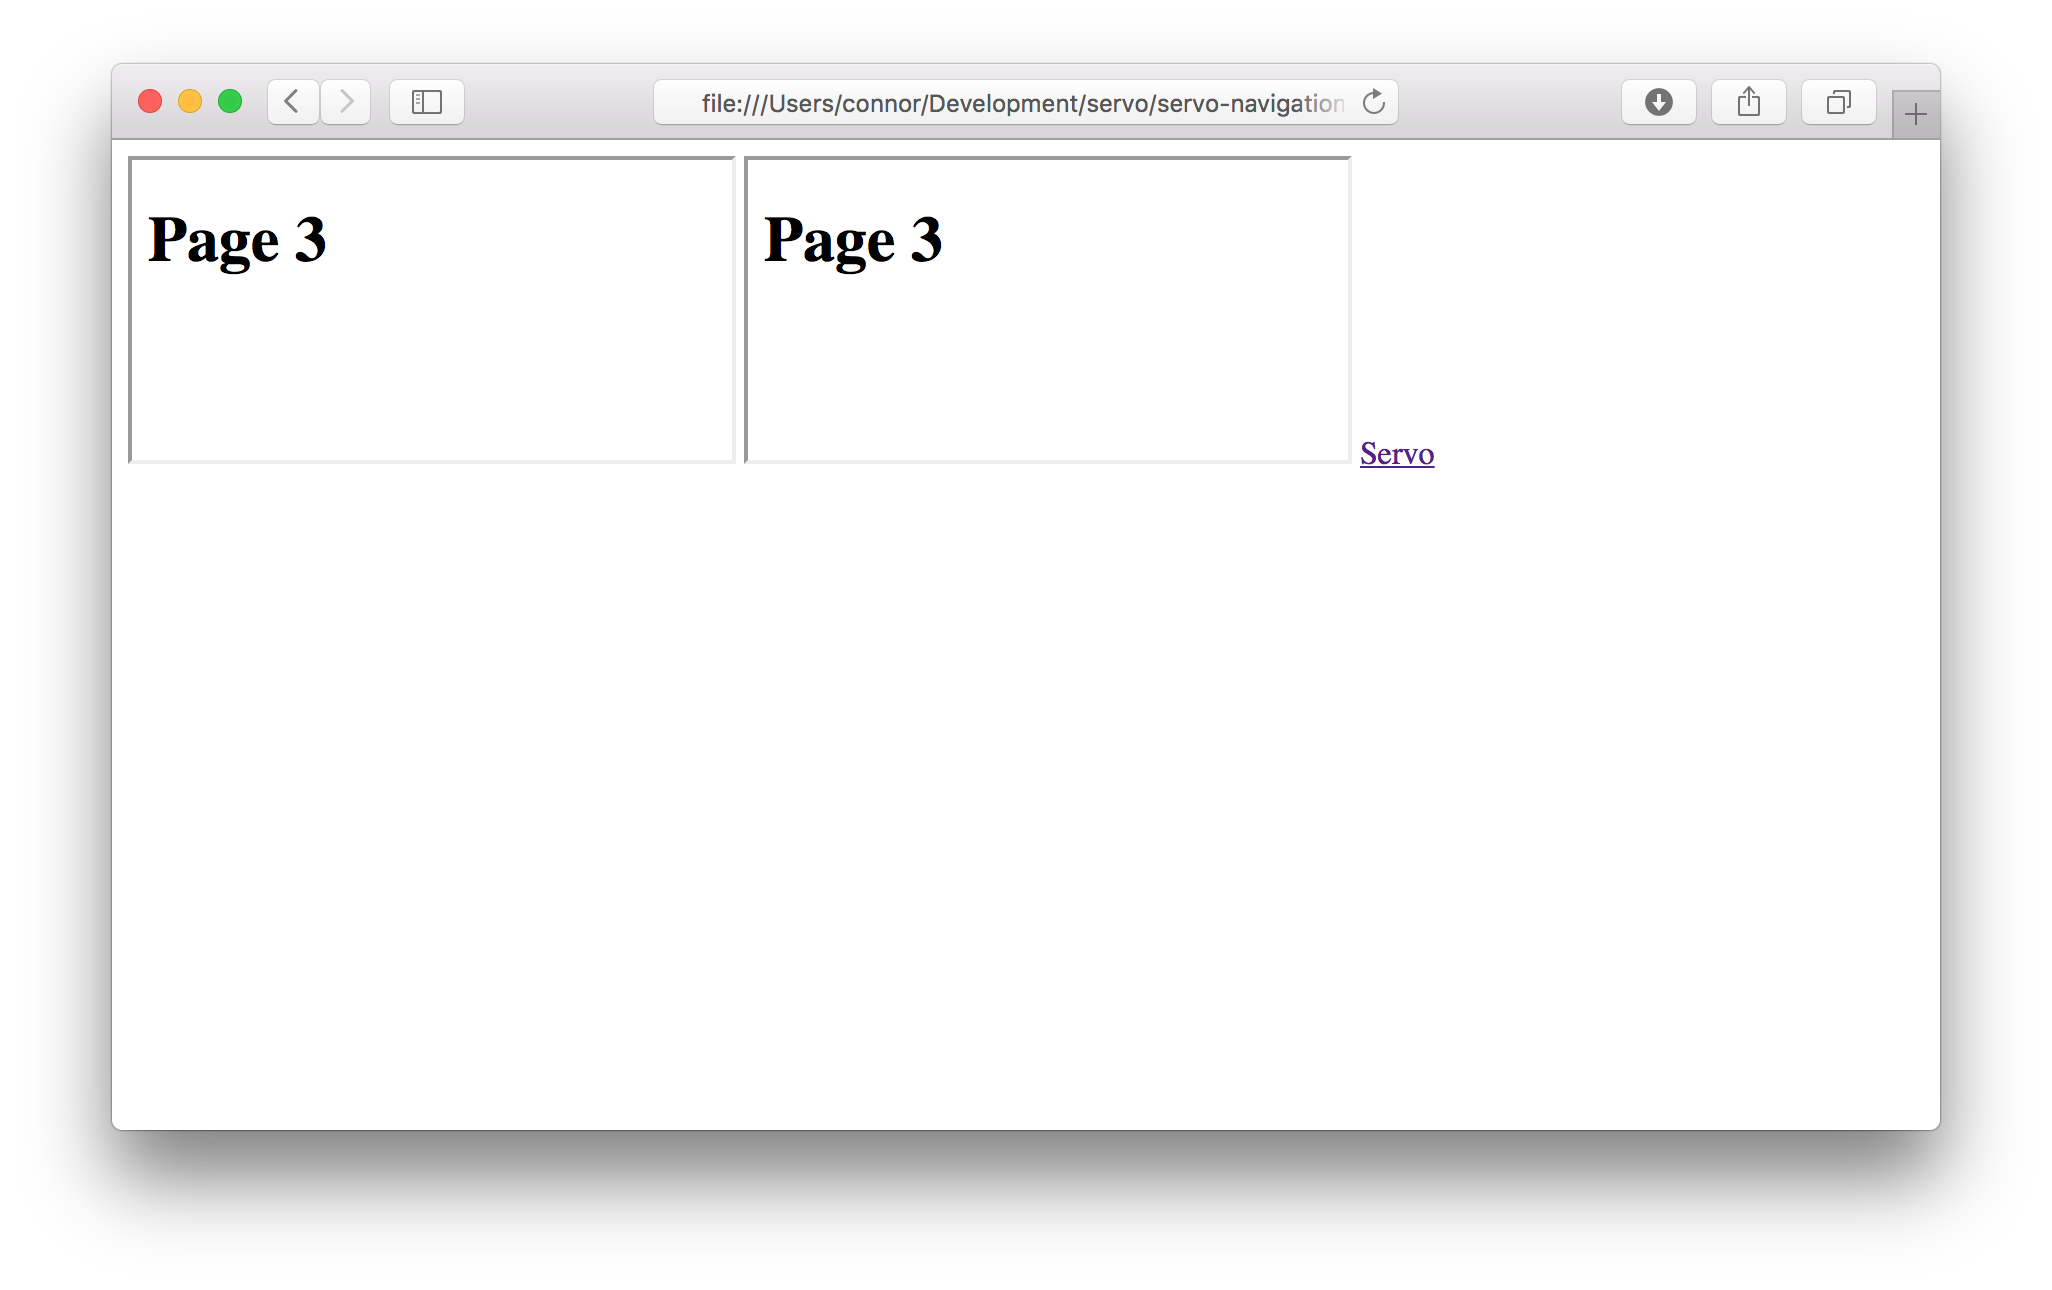
\includegraphics[width=.5\linewidth]{images/experiments/forwardback4/safari/7.png}
    }~\raisebox{-.5\height}{
      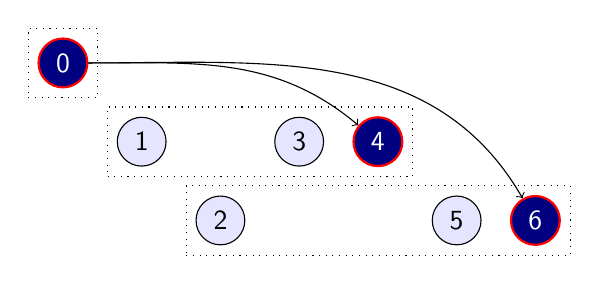
\begin{tikzpicture}
        \node[doc,active,fully](0) at (0,0){0};
        \node[doc](1) at (1,-1){1};
        \node[doc](2) at (2,-2){2};
        \node[doc](3) at (3,-1){3};
        \node[doc,active,fully](4) at (4,-1){4};
        \node[doc](5) at (5,-2){5};
        \node[doc,jshactive,fully](6) at (6,-2){6};
        \node[draw,dotted,fit=(0)]{};
        \node[draw,dotted,fit=(1)(4)]{};
        \node[draw,dotted,fit=(2)(6)]{};
        \draw[->](0)to[out=0,in=140](4);
        \draw[->](0)to[out=0,in=120](6);
      \end{tikzpicture}
    }
    \caption{Traversal by $4$.}
  \end{figure}

  These results in Safari satisfy Goal~\ref{goal:homomorphism}.

  Chrome:
  \begin{figure}[H]
    \raisebox{-.5\height}{
      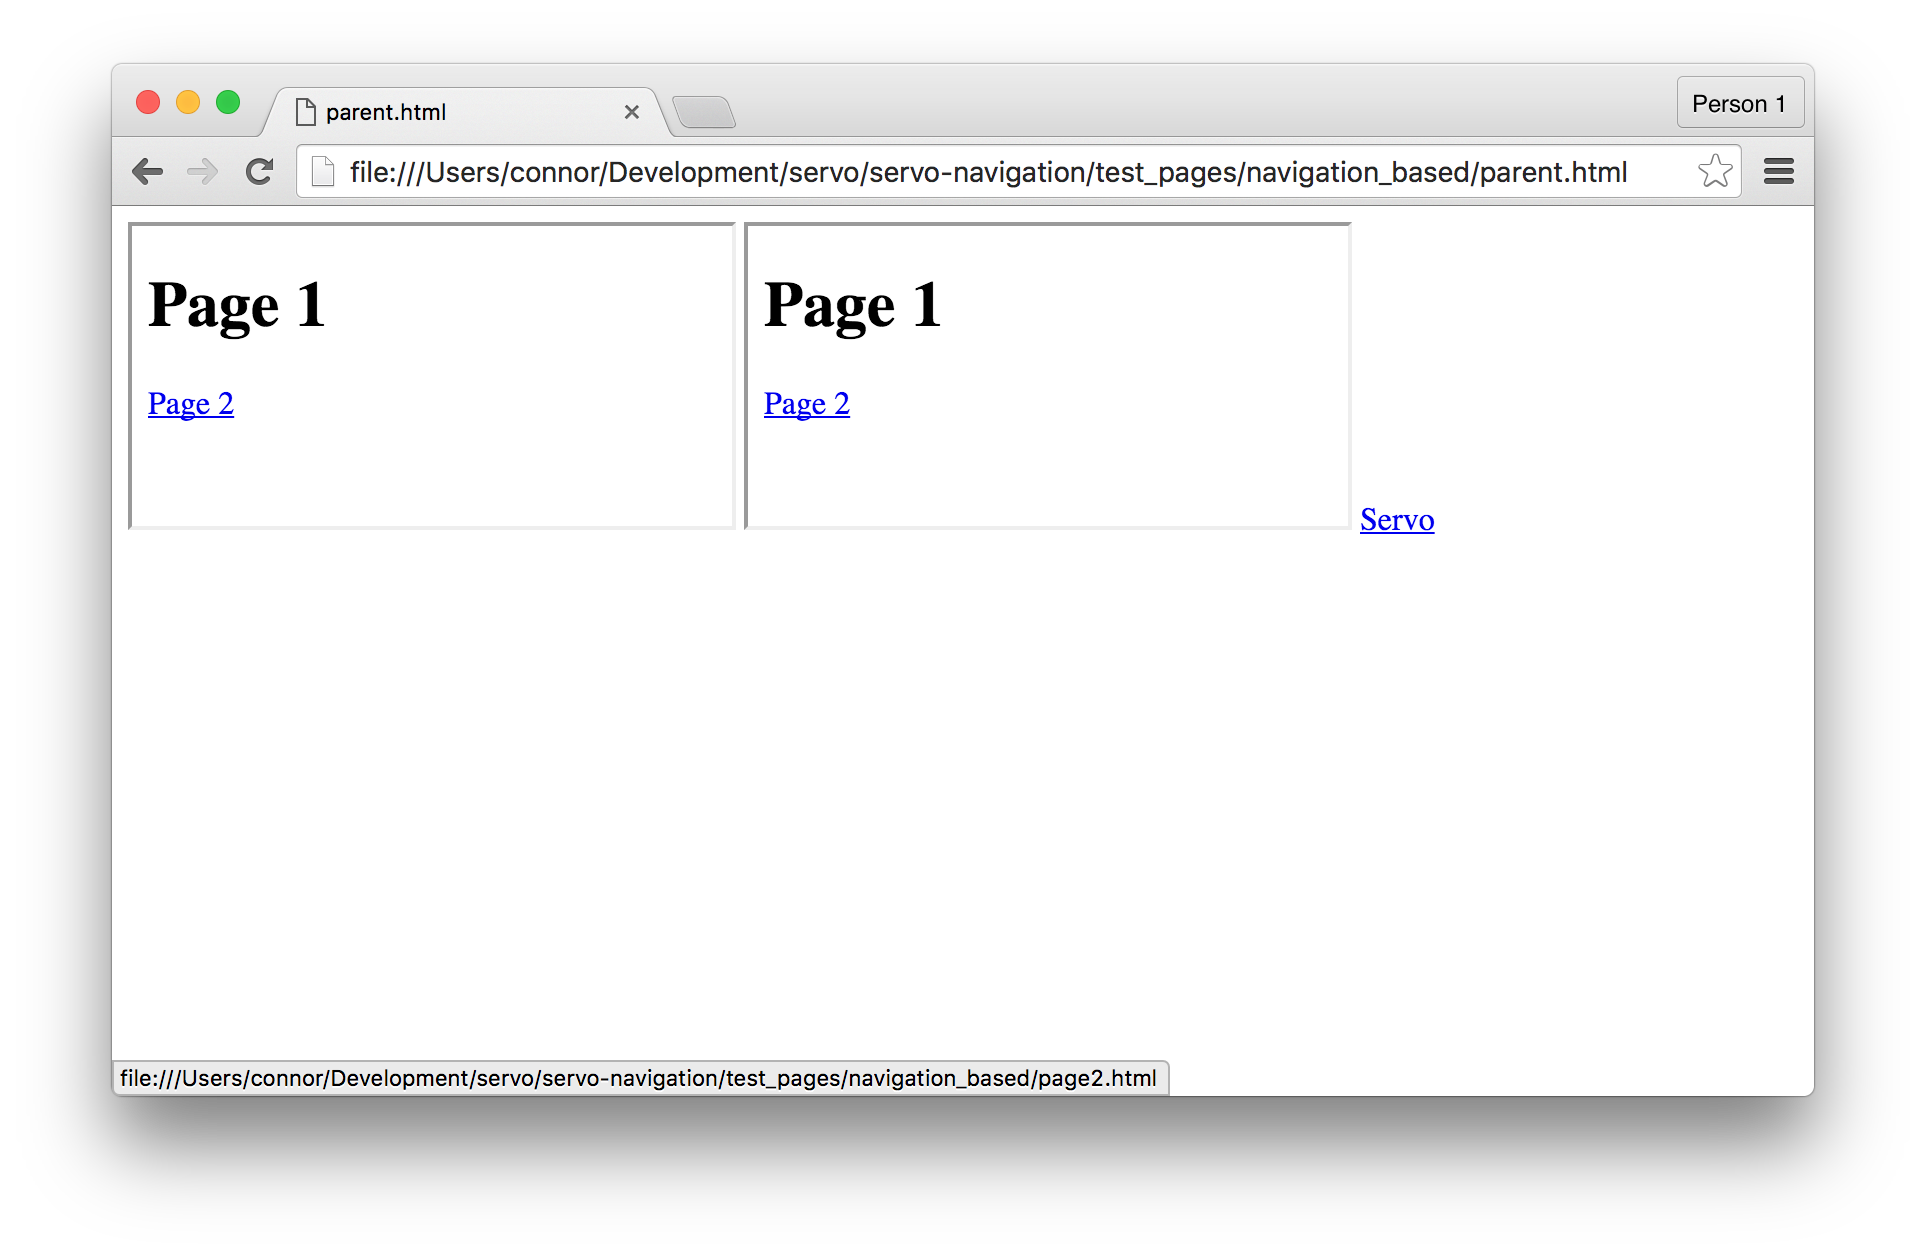
\includegraphics[width=.5\linewidth]{images/experiments/forwardback4/chrome/1.png}%
    }~\raisebox{-.5\height}{
      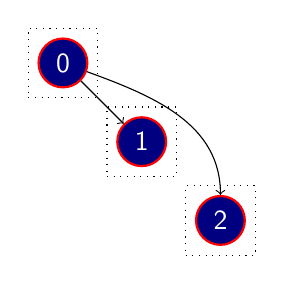
\begin{tikzpicture}
        \node[doc,active,fully](0) at (0,0){0};
        \node[doc,active,fully](1) at (1,-1){1};
        \node[doc,jshactive,fully](2) at (2,-2){2};
        \node[draw,dotted,fit=(0)]{};
        \node[draw,dotted,fit=(1)]{};
        \node[draw,dotted,fit=(2)]{};
        \draw[->](0)--(1);
        \draw[->](0)to[out=-20,in=90](2);
      \end{tikzpicture}
    }
    \caption{Initial State}
  \end{figure}

  Navigate document $1$ to Page 2:
  \begin{figure}[H]
    \raisebox{-.5\height}{
      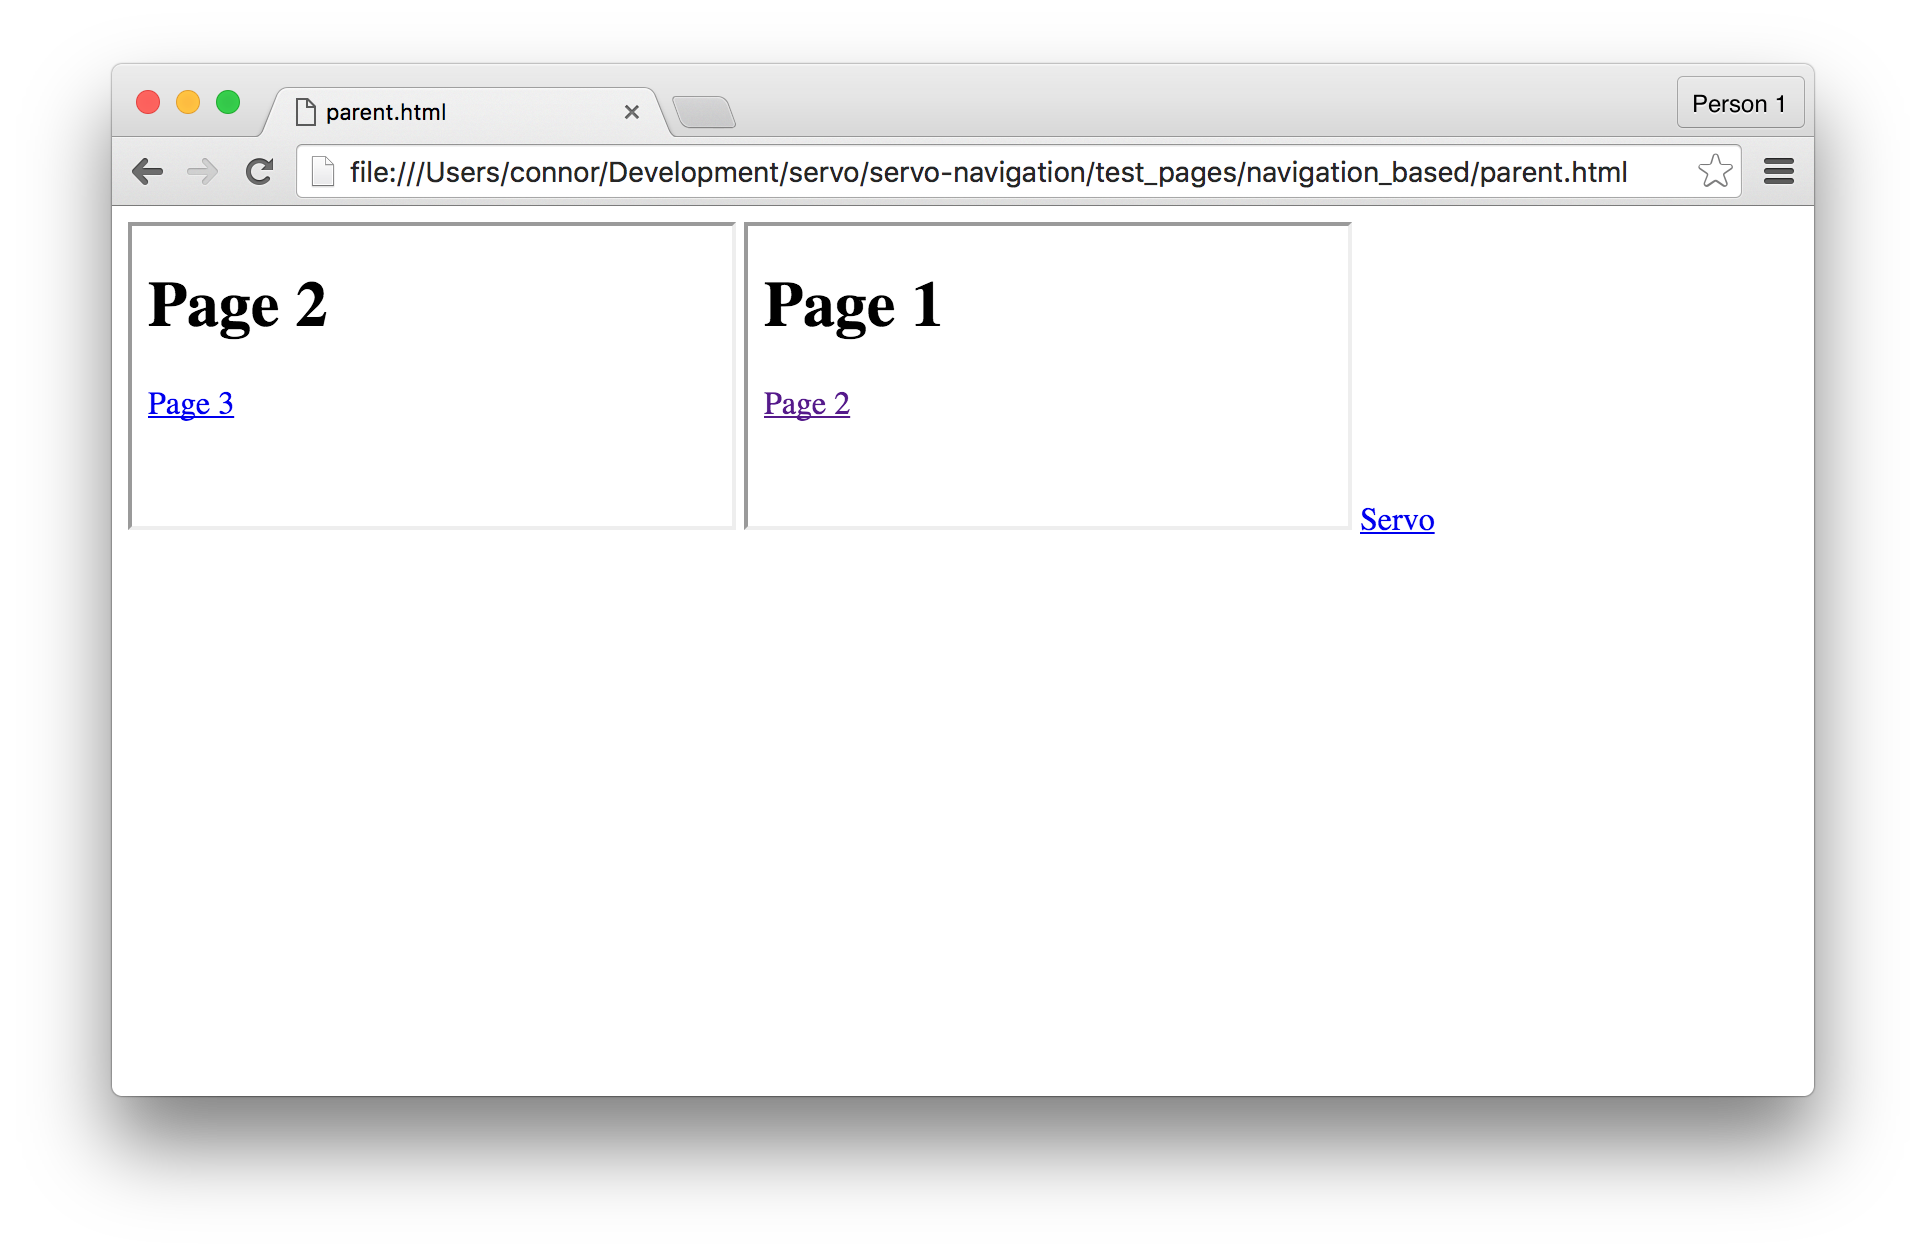
\includegraphics[width=.5\linewidth]{images/experiments/forwardback4/chrome/2.png}
    }~\raisebox{-.5\height}{
      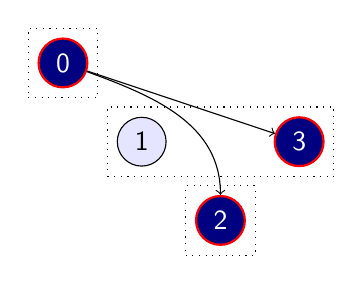
\begin{tikzpicture}
        \node[doc,active,fully](0) at (0,0){0};
        \node[doc](1) at (1,-1){1};
        \node[doc,active,fully](2) at (2,-2){2};
        \node[doc,jshactive,fully](3) at (3,-1){3};
        \node[draw,dotted,fit=(0)]{};
        \node[draw,dotted,fit=(1)(3)]{};
        \node[draw,dotted,fit=(2)]{};
        \draw[->](0)--(3);
        \draw[->](0)to[out=-20,in=90](2);
      \end{tikzpicture}
    }
    \caption{Navigate document $1$ to Page 2.}
  \end{figure}

  Navigate document $3$ to Page 3:
  \begin{figure}[H]
    \raisebox{-.5\height}{
      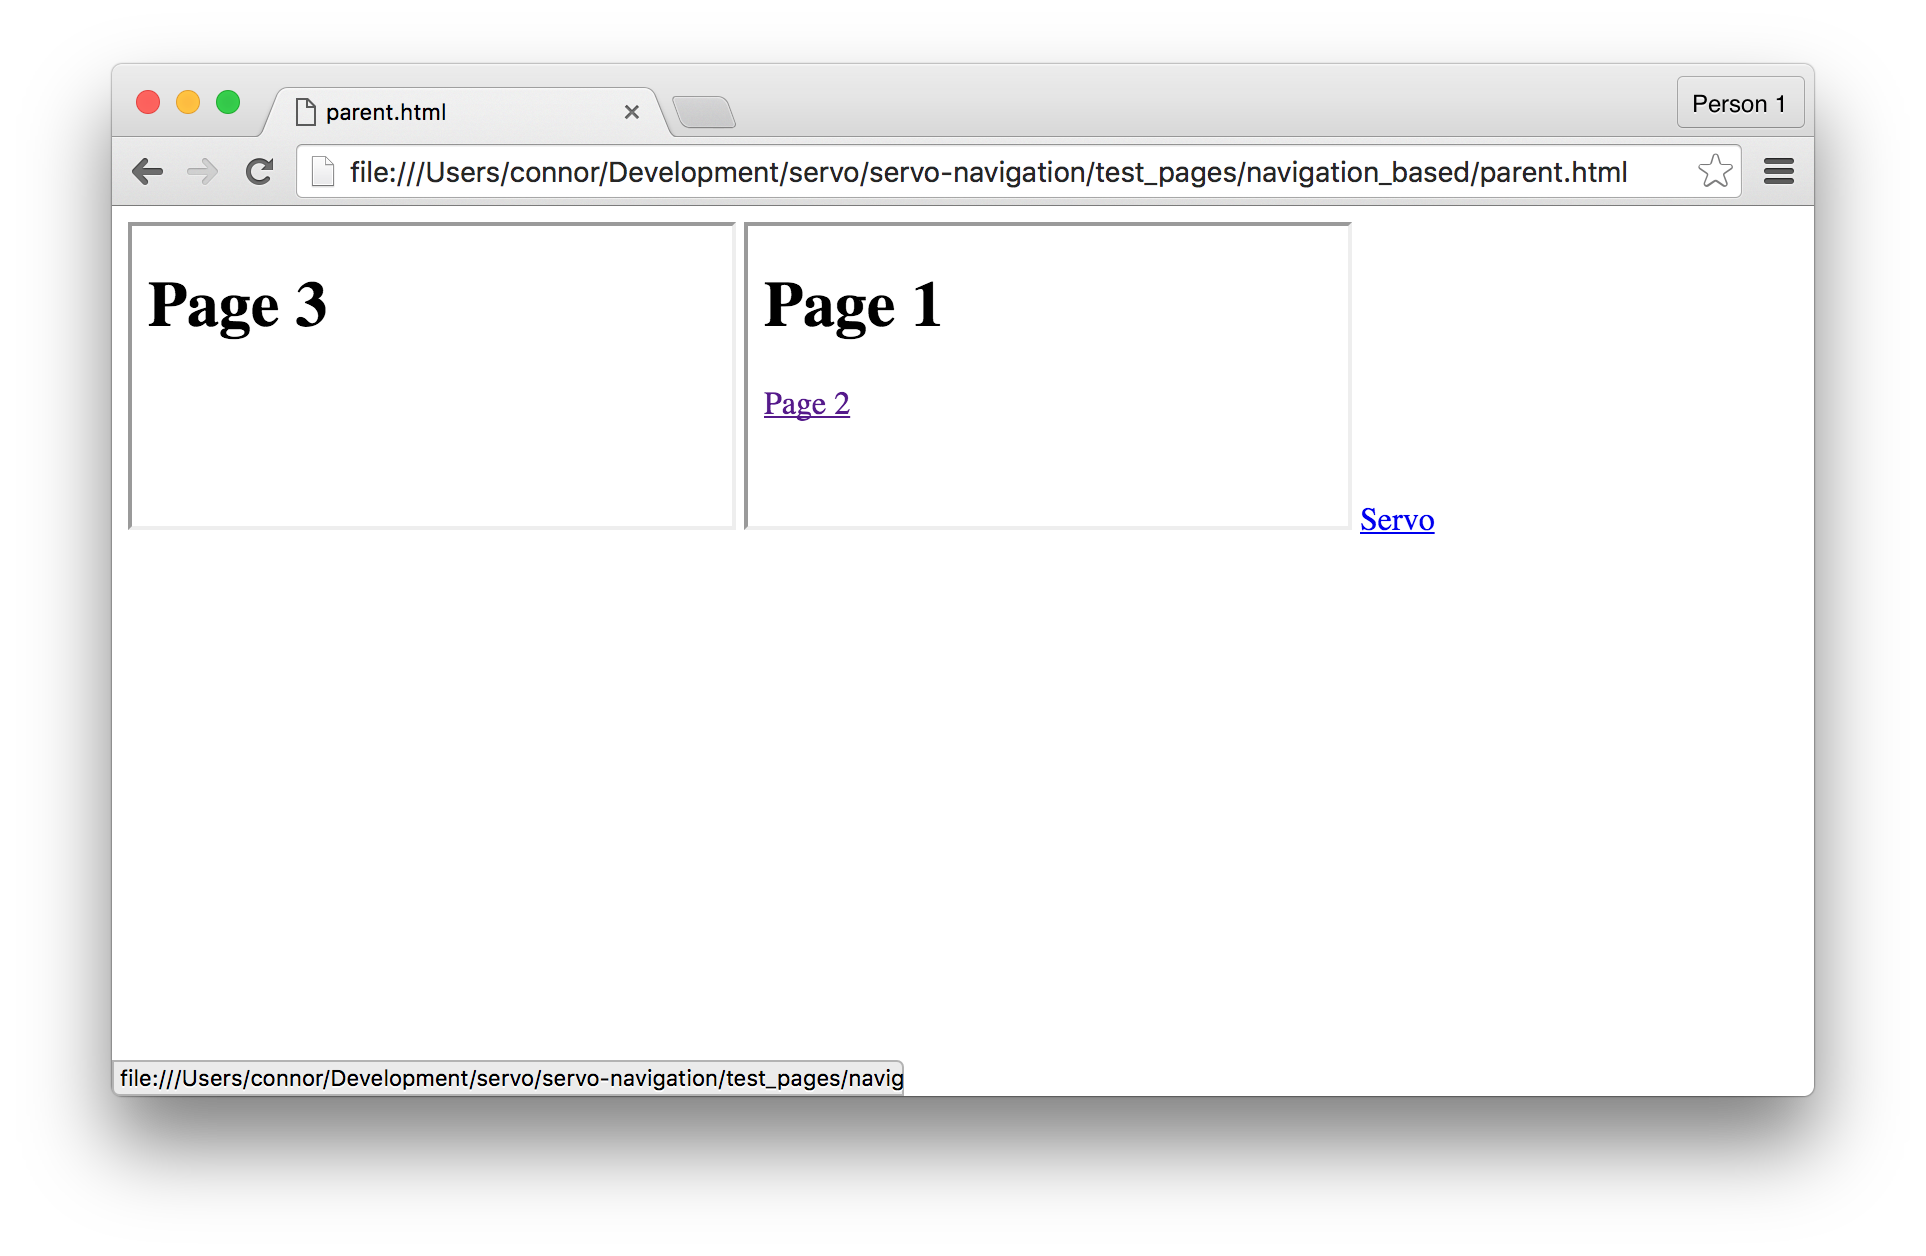
\includegraphics[width=.5\linewidth]{images/experiments/forwardback4/chrome/3.png}
    }~\raisebox{-.5\height}{
      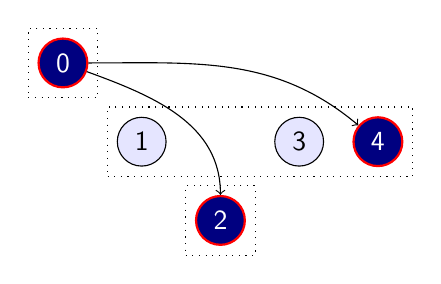
\begin{tikzpicture}
        \node[doc,active,fully](0) at (0,0){0};
        \node[doc](1) at (1,-1){1};
        \node[doc,active,fully](2) at (2,-2){2};
        \node[doc](3) at (3,-1){3};
        \node[doc,jshactive,fully](4) at (4,-1){4};
        \node[draw,dotted,fit=(0)]{};
        \node[draw,dotted,fit=(1)(4)]{};
        \node[draw,dotted,fit=(2)]{};
        \draw[->](0)to[out=0,in=140](4);
        \draw[->](0)to[out=-20,in=90](2);
      \end{tikzpicture}
    }
    \caption{Navigate document $3$ to Page 3.}
  \end{figure}

  Navigate document $2$ to Page 2:
  \begin{figure}[H]
    \raisebox{-.5\height}{
      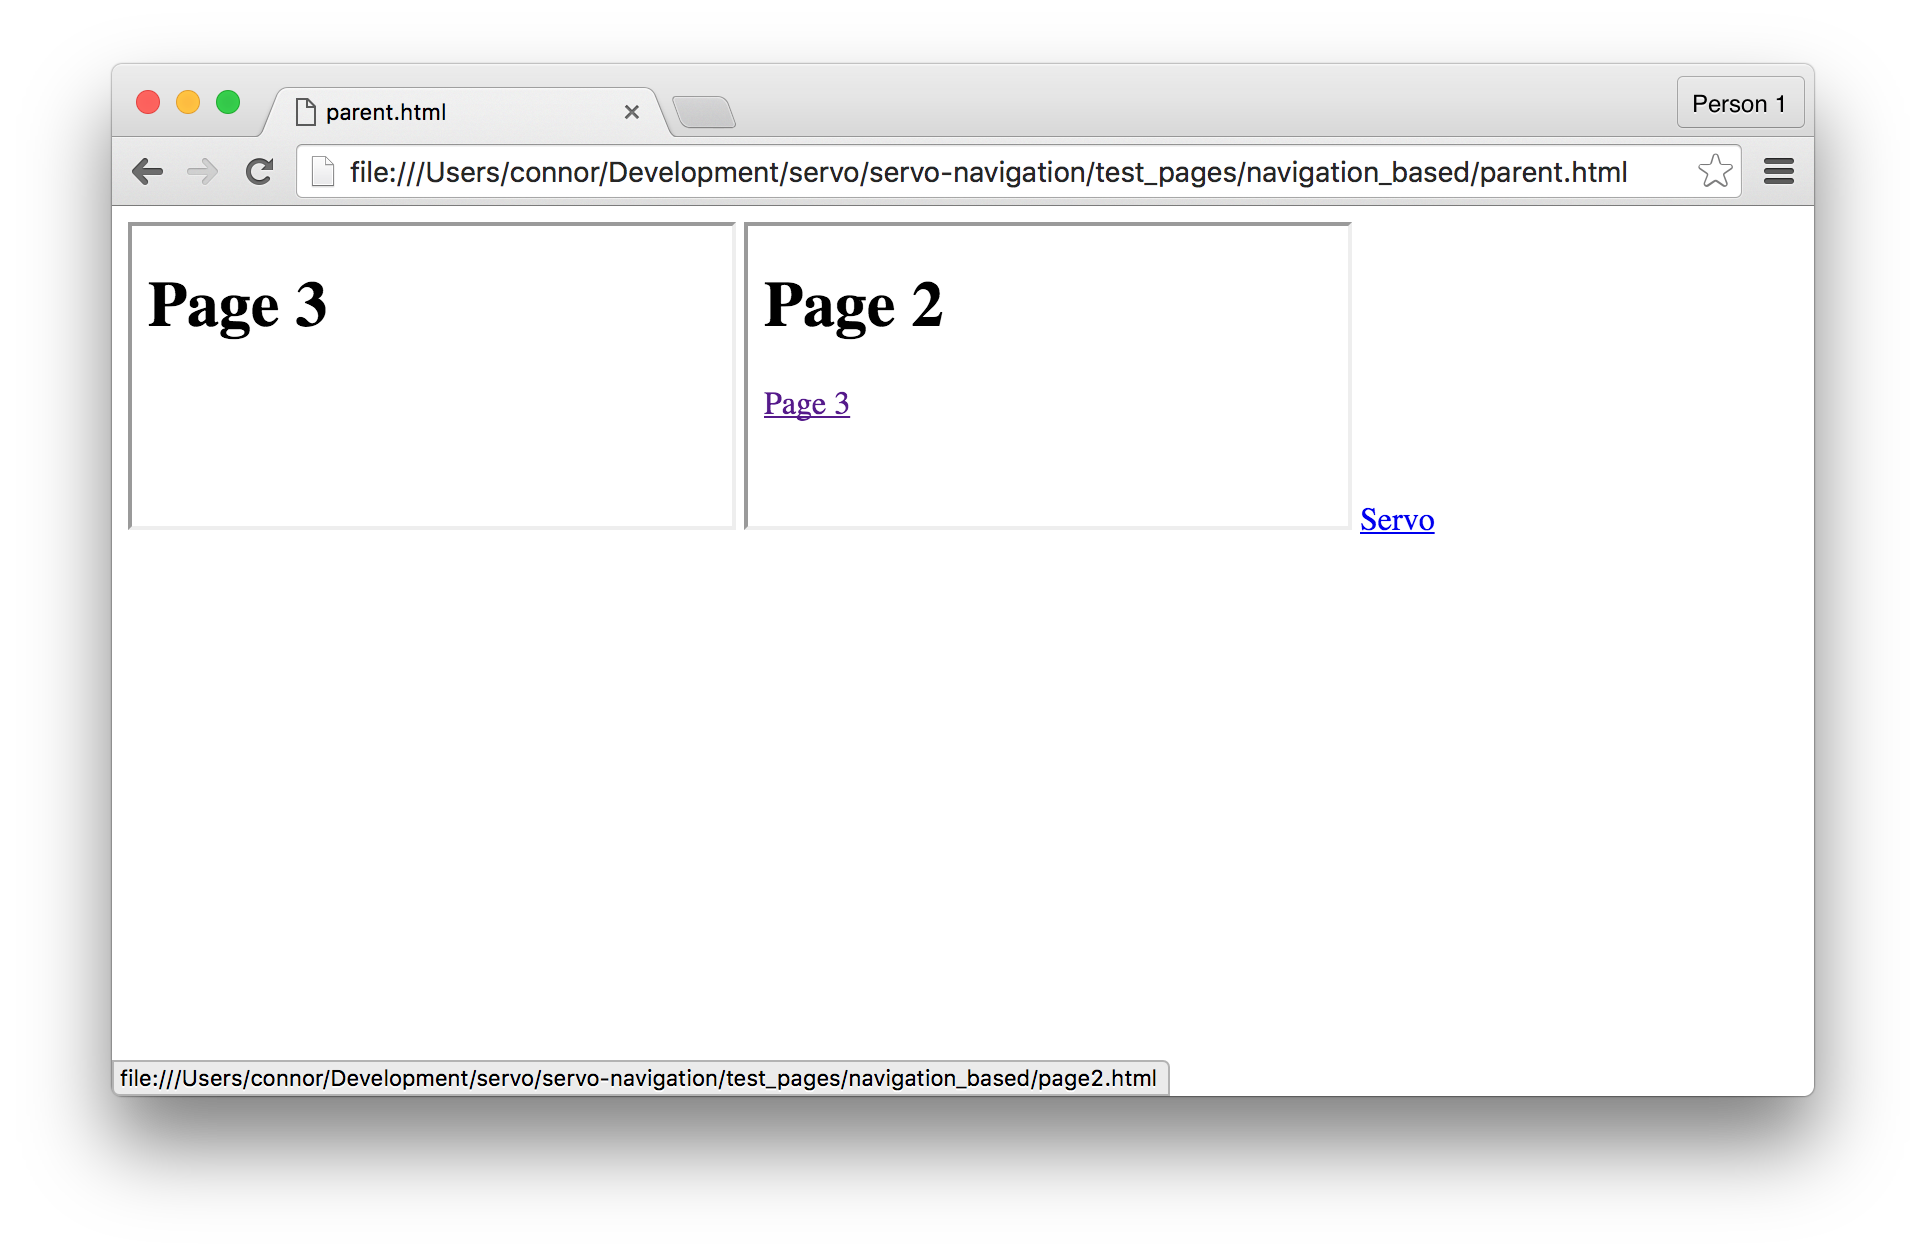
\includegraphics[width=.5\linewidth]{images/experiments/forwardback4/chrome/4.png}
    }~\raisebox{-.5\height}{
      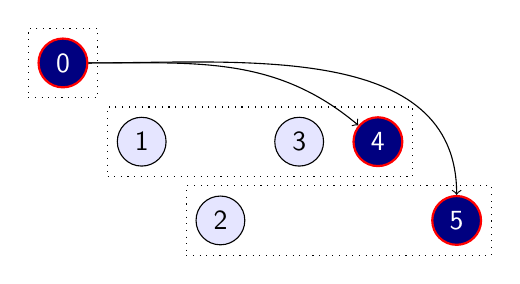
\begin{tikzpicture}
        \node[doc,active,fully](0) at (0,0){0};
        \node[doc](1) at (1,-1){1};
        \node[doc](2) at (2,-2){2};
        \node[doc](3) at (3,-1){3};
        \node[doc,active,fully](4) at (4,-1){4};
        \node[doc,jshactive,fully](5) at (5,-2){5};
        \node[draw,dotted,fit=(0)]{};
        \node[draw,dotted,fit=(1)(4)]{};
        \node[draw,dotted,fit=(2)(5)]{};
        \draw[->](0)to[out=0,in=140](4);
        \draw[->](0)to[out=0,in=90](5);
      \end{tikzpicture}
    }
    \caption{Navigate document $2$ to Page 2.}
  \end{figure}

  Navigate document $5$ to Page 3:
  \begin{figure}[H]
    \raisebox{-.5\height}{
      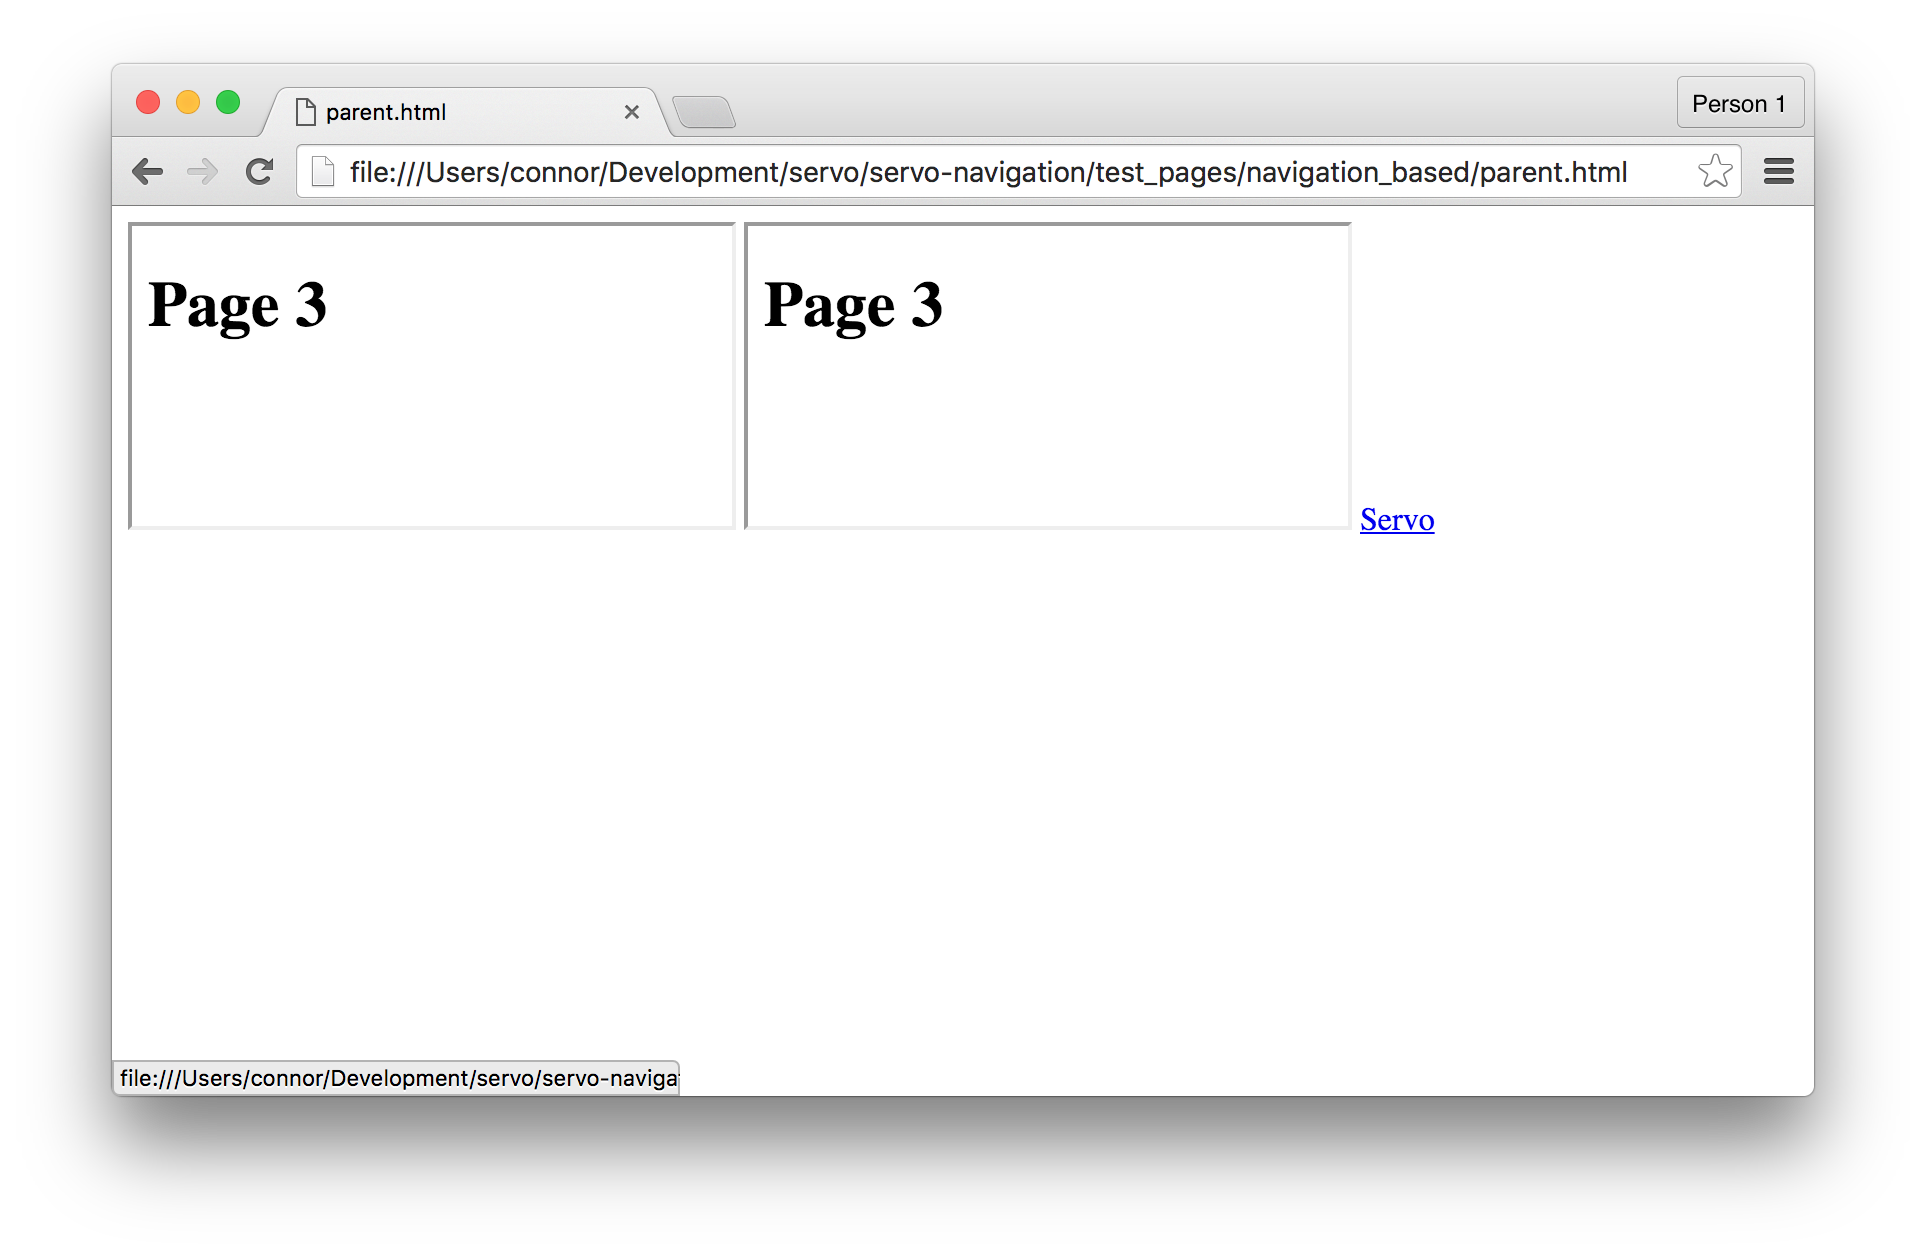
\includegraphics[width=.5\linewidth]{images/experiments/forwardback4/chrome/5.png}
    }~\raisebox{-.5\height}{
      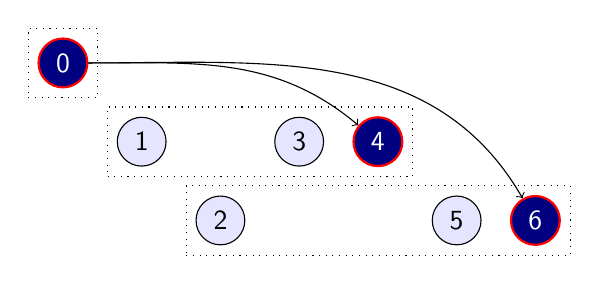
\begin{tikzpicture}
        \node[doc,active,fully](0) at (0,0){0};
        \node[doc](1) at (1,-1){1};
        \node[doc](2) at (2,-2){2};
        \node[doc](3) at (3,-1){3};
        \node[doc,active,fully](4) at (4,-1){4};
        \node[doc](5) at (5,-2){5};
        \node[doc,jshactive,fully](6) at (6,-2){6};
        \node[draw,dotted,fit=(0)]{};
        \node[draw,dotted,fit=(1)(4)]{};
        \node[draw,dotted,fit=(2)(6)]{};
        \draw[->](0)to[out=0,in=140](4);
        \draw[->](0)to[out=0,in=120](6);
      \end{tikzpicture}
    }
    \caption{Navigate document $5$ to Page 3.}
  \end{figure}

  \emph{$\aNH$ traverses the history by $-4$ to $\aNH'$}:
  \begin{figure}[H]
    \raisebox{-.5\height}{
      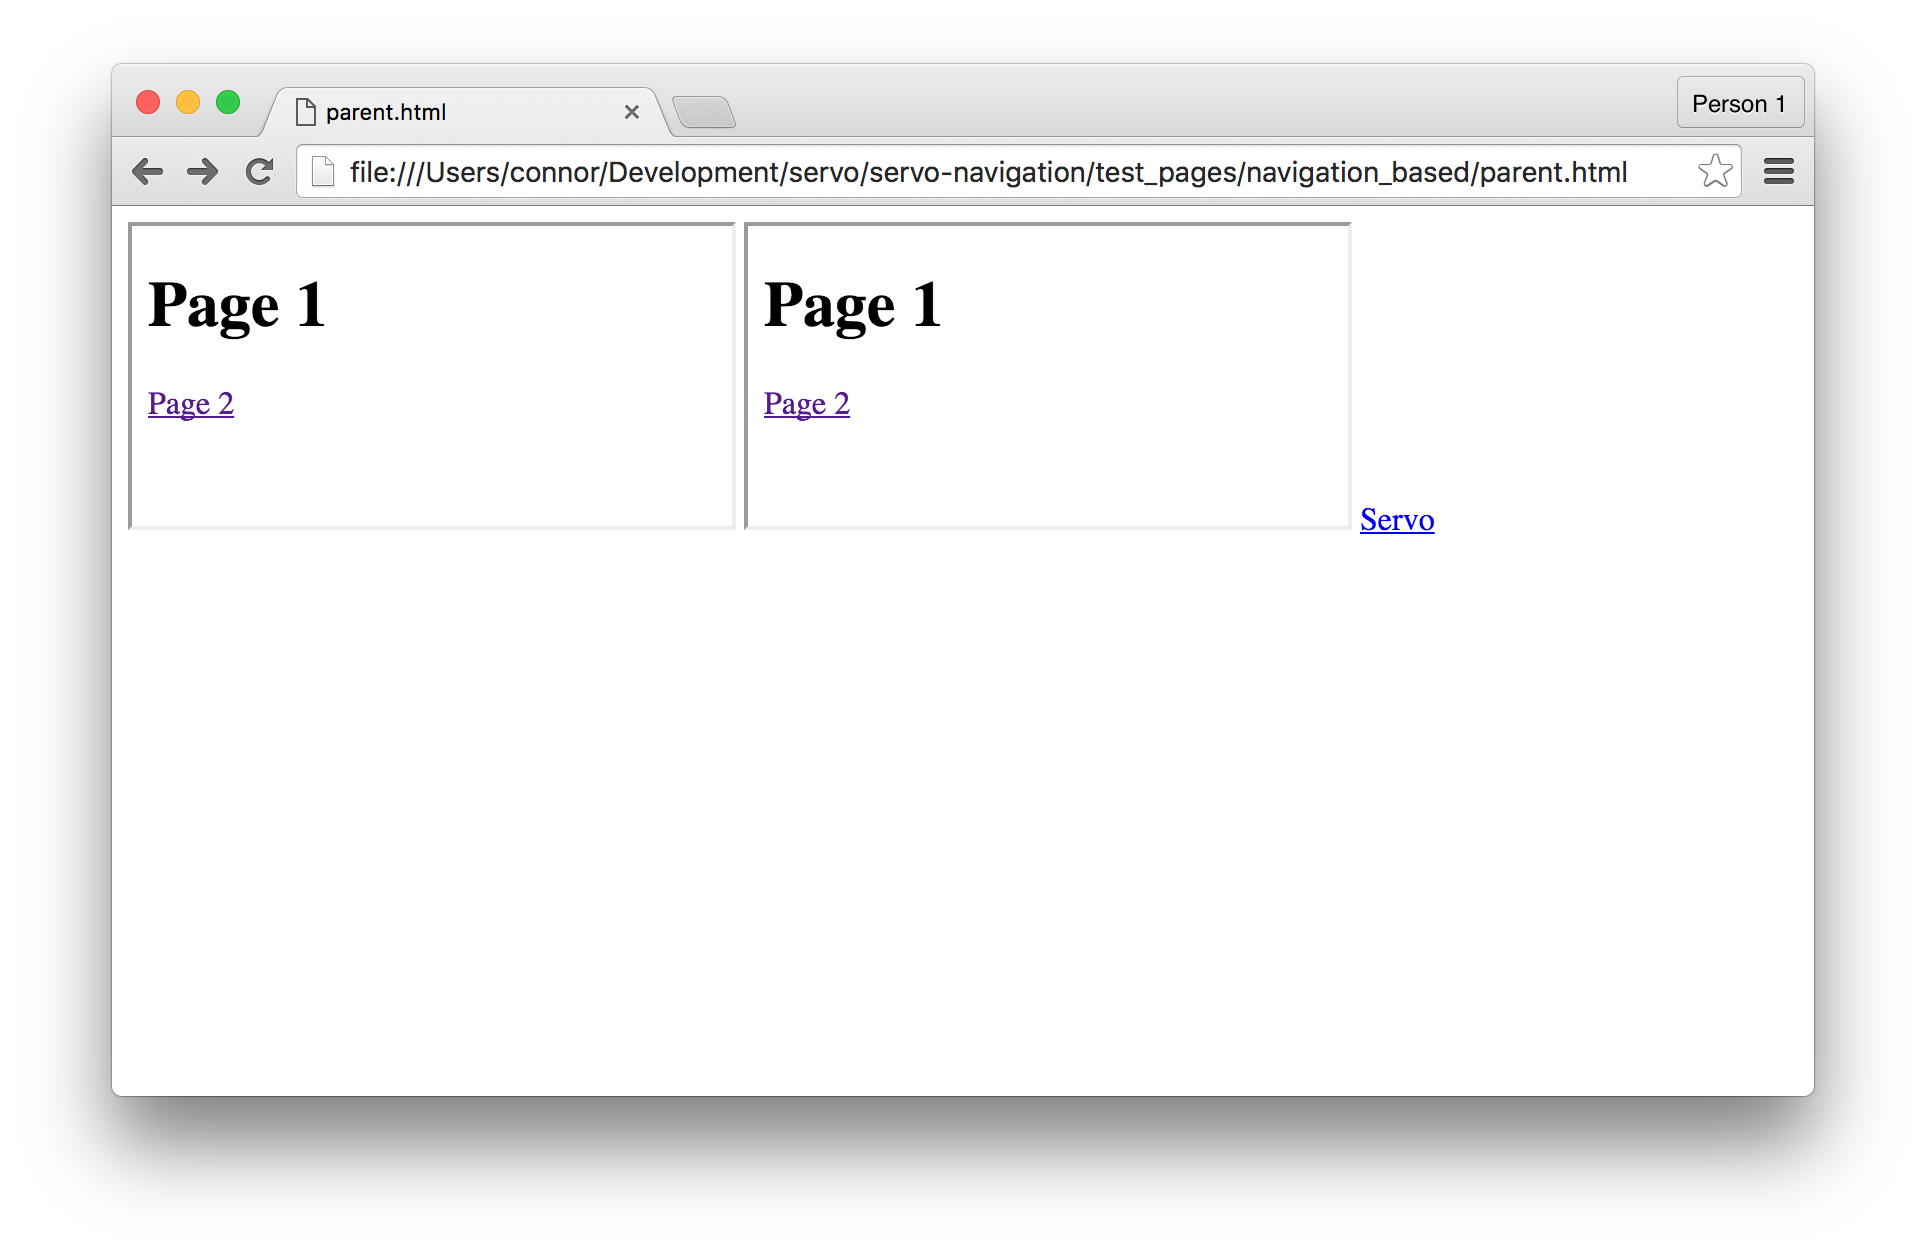
\includegraphics[width=.5\linewidth]{images/experiments/forwardback4/chrome/6.png}
    }~\raisebox{-.5\height}{
      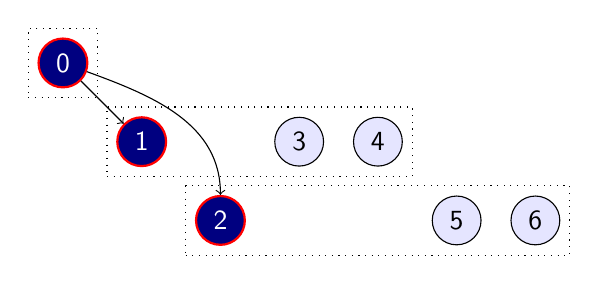
\begin{tikzpicture}
        \node[doc,active,fully](0) at (0,0){0};
        \node[doc,active,fully](1) at (1,-1){1};
        \node[doc,jshactive,fully](2) at (2,-2){2};
        \node[doc](3) at (3,-1){3};
        \node[doc](4) at (4,-1){4};
        \node[doc](5) at (5,-2){5};
        \node[doc](6) at (6,-2){6};
        \node[draw,dotted,fit=(0)]{};
        \node[draw,dotted,fit=(1)(4)]{};
        \node[draw,dotted,fit=(2)(6)]{};
        \draw[->](0)--(1);
        \draw[->](0)to[out=-20,in=90](2);
      \end{tikzpicture}
    }
    \caption{Traversal by $-4$.}
  \end{figure}

  \emph{$\aNH'$ traverses the history by $4$ to $\aNH''$}:
  \begin{figure}[H]
    \raisebox{-.5\height}{
      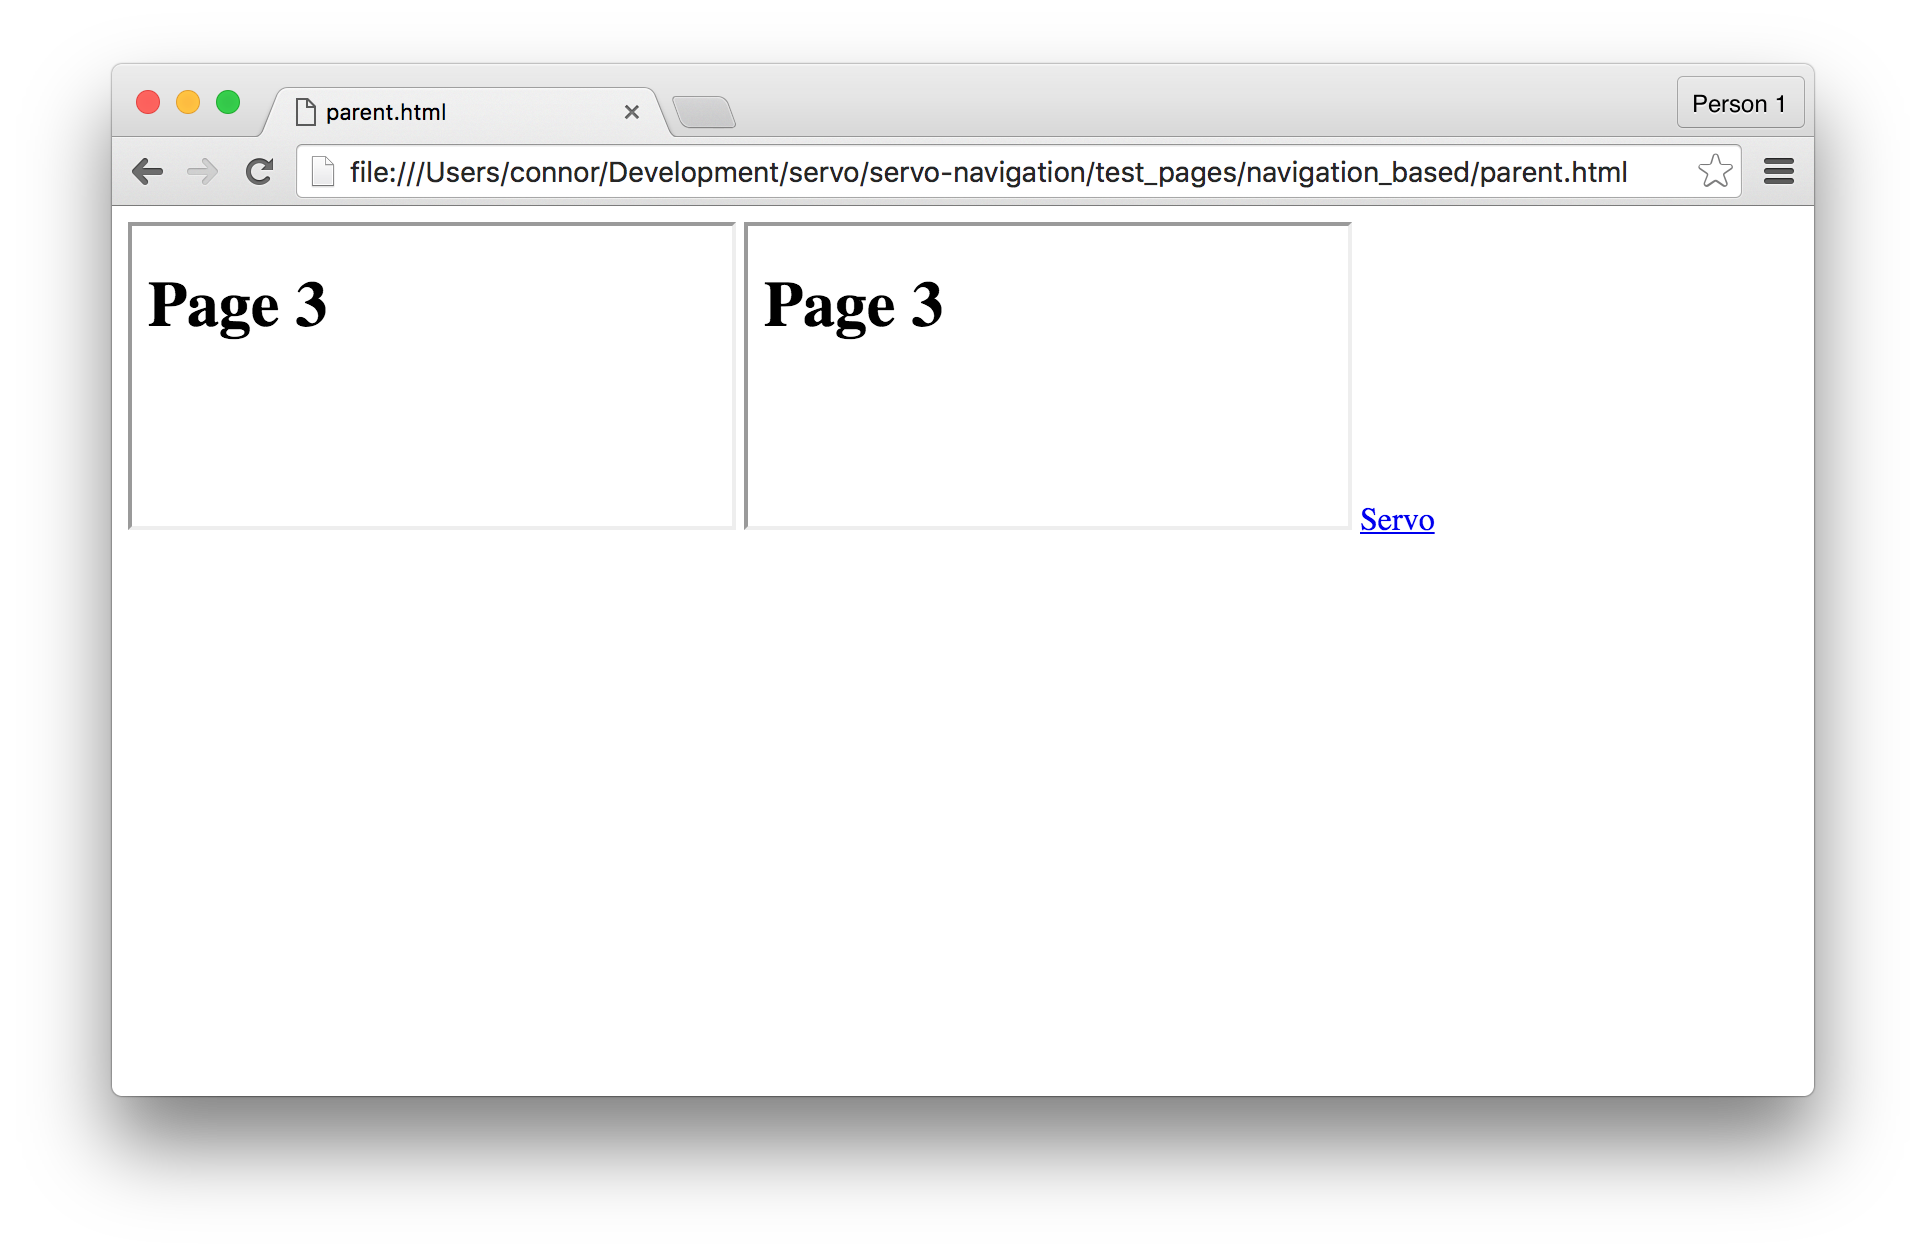
\includegraphics[width=.5\linewidth]{images/experiments/forwardback4/chrome/7.png}
    }~\raisebox{-.5\height}{
      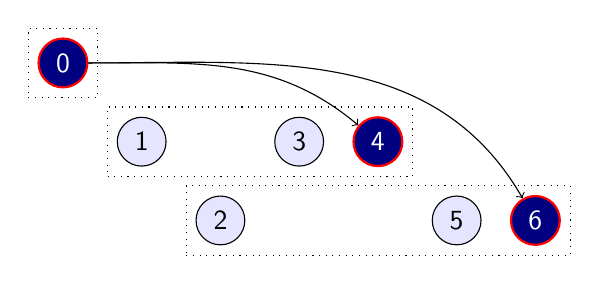
\begin{tikzpicture}
        \node[doc,active,fully](0) at (0,0){0};
        \node[doc](1) at (1,-1){1};
        \node[doc](2) at (2,-2){2};
        \node[doc](3) at (3,-1){3};
        \node[doc,active,fully](4) at (4,-1){4};
        \node[doc](5) at (5,-2){5};
        \node[doc,jshactive,fully](6) at (6,-2){6};
        \node[draw,dotted,fit=(0)]{};
        \node[draw,dotted,fit=(1)(4)]{};
        \node[draw,dotted,fit=(2)(6)]{};
        \draw[->](0)to[out=0,in=140](4);
        \draw[->](0)to[out=0,in=120](6);
      \end{tikzpicture}
    }
    \caption{Traversal by $4$.}
  \end{figure}

  These results in Chrome satisfy Goal~\ref{goal:homomorphism}.
\end{experiment}

\begin{experiment}
  In this experiment $pushState$ and $replaceState$ traversals are tested against Goal~\ref{goal:homomorphism}.

  Firefox:
  \begin{figure}[H]
    \raisebox{-.5\height}{
      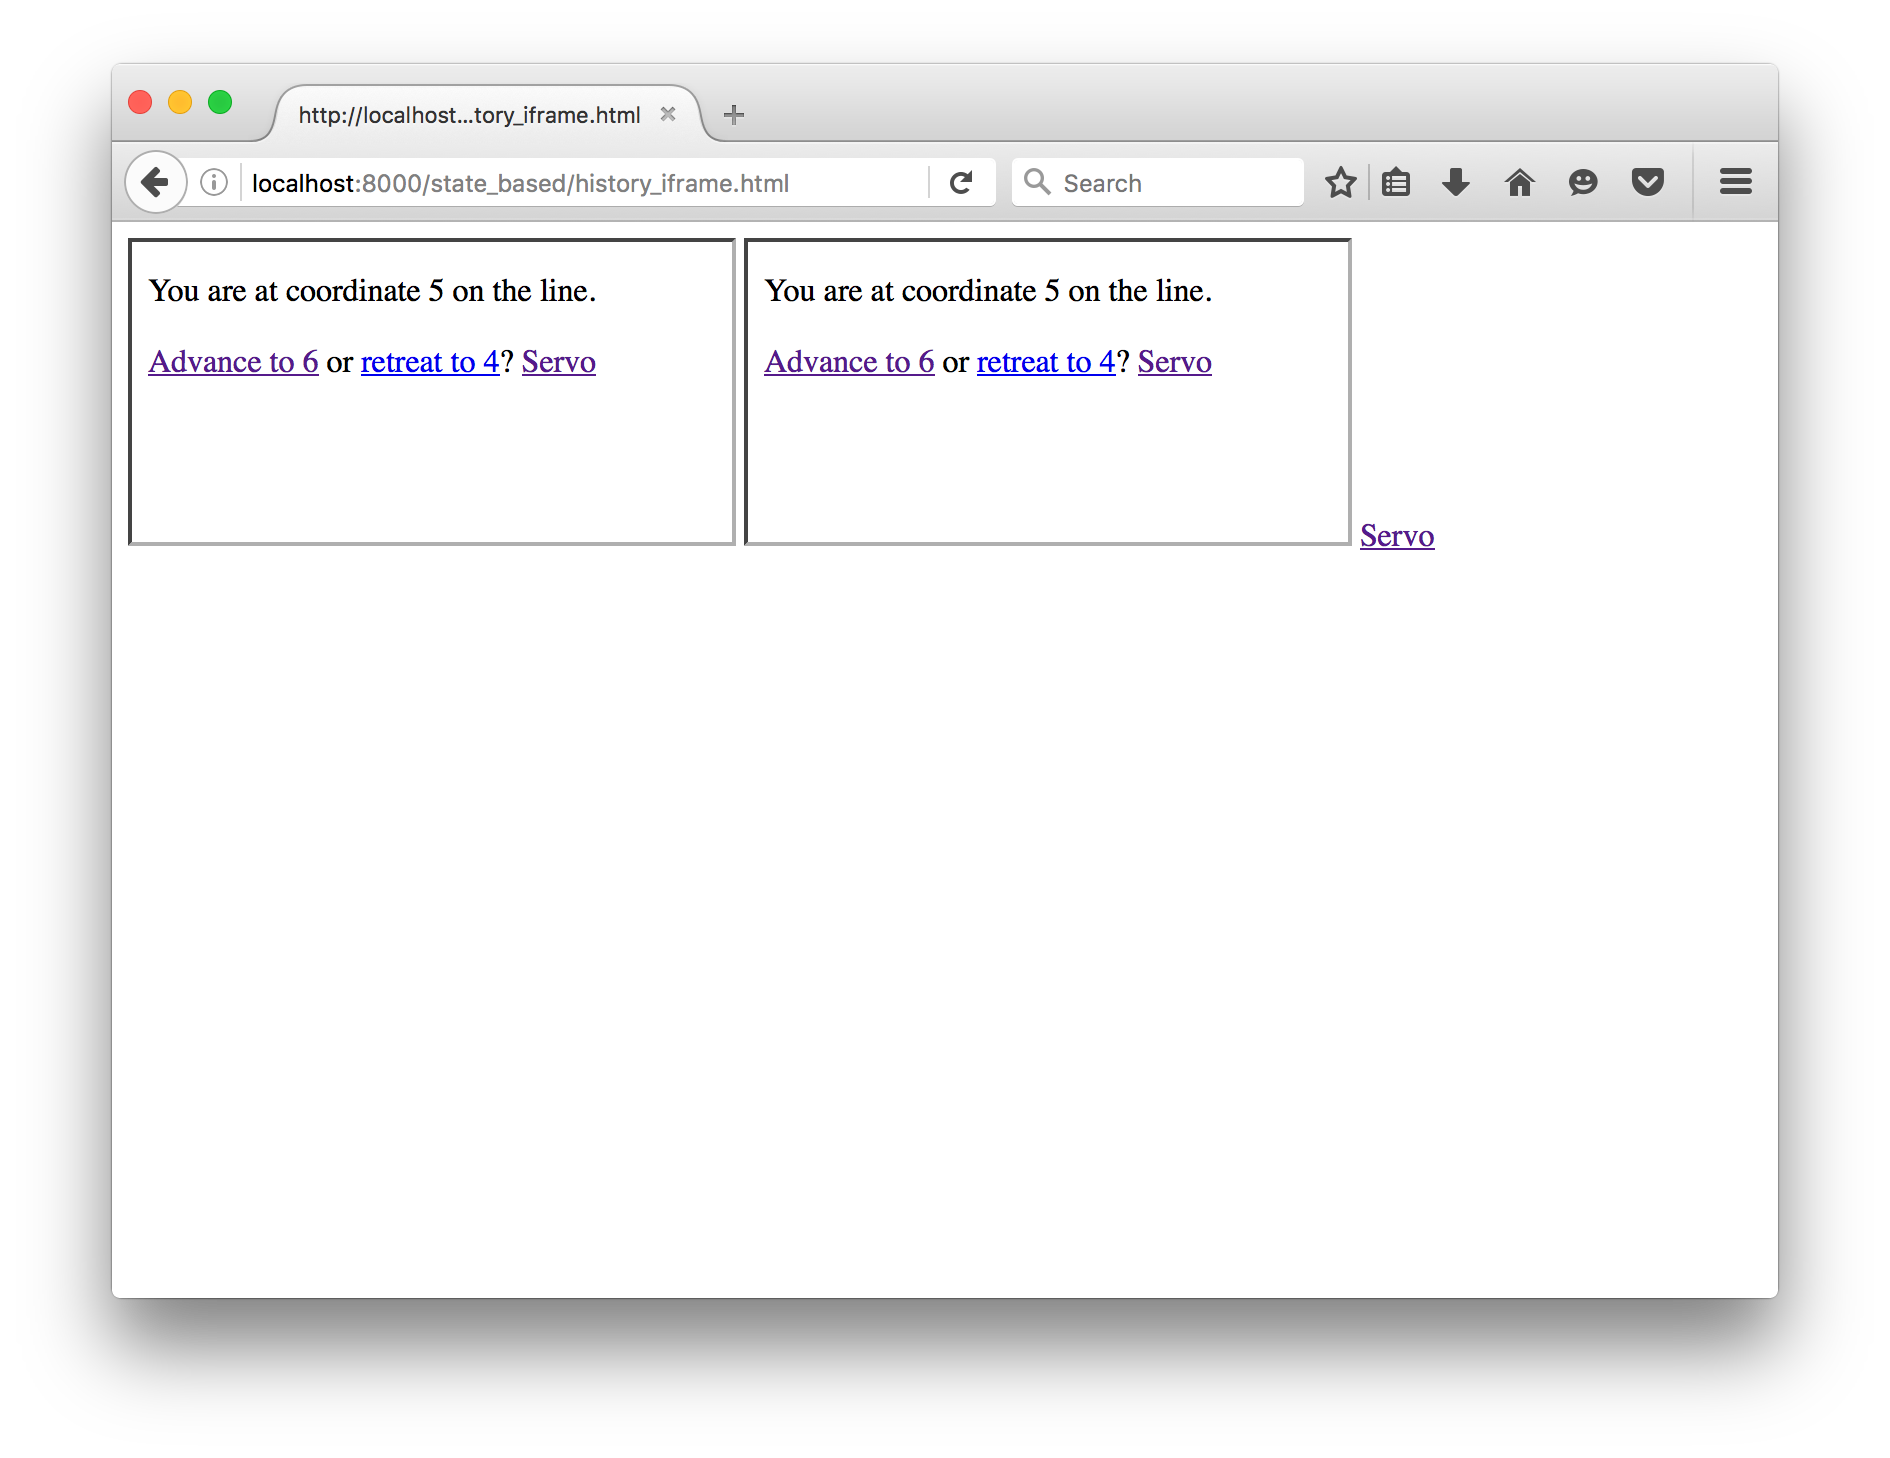
\includegraphics[width=.5\linewidth]{images/experiments/forwardback4state/firefox/1.png}%
    }~\raisebox{-.5\height}{
      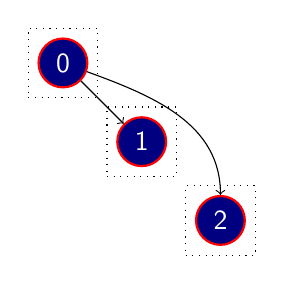
\begin{tikzpicture}
        \node[doc,active,fully](0) at (0,0){0};
        \node[doc,active,fully](1) at (1,-1){1};
        \node[doc,jshactive,fully](2) at (2,-2){2};
        \node[draw,dotted,fit=(0)]{};
        \node[draw,dotted,fit=(1)]{};
        \node[draw,dotted,fit=(2)]{};
        \draw[->](0)--(1);
        \draw[->](0)to[out=-20,in=90](2);
      \end{tikzpicture}
    }
    \caption{Initial State}
  \end{figure}

  Advance document 1 to $6$:
  \begin{figure}[H]
    \raisebox{-.5\height}{
      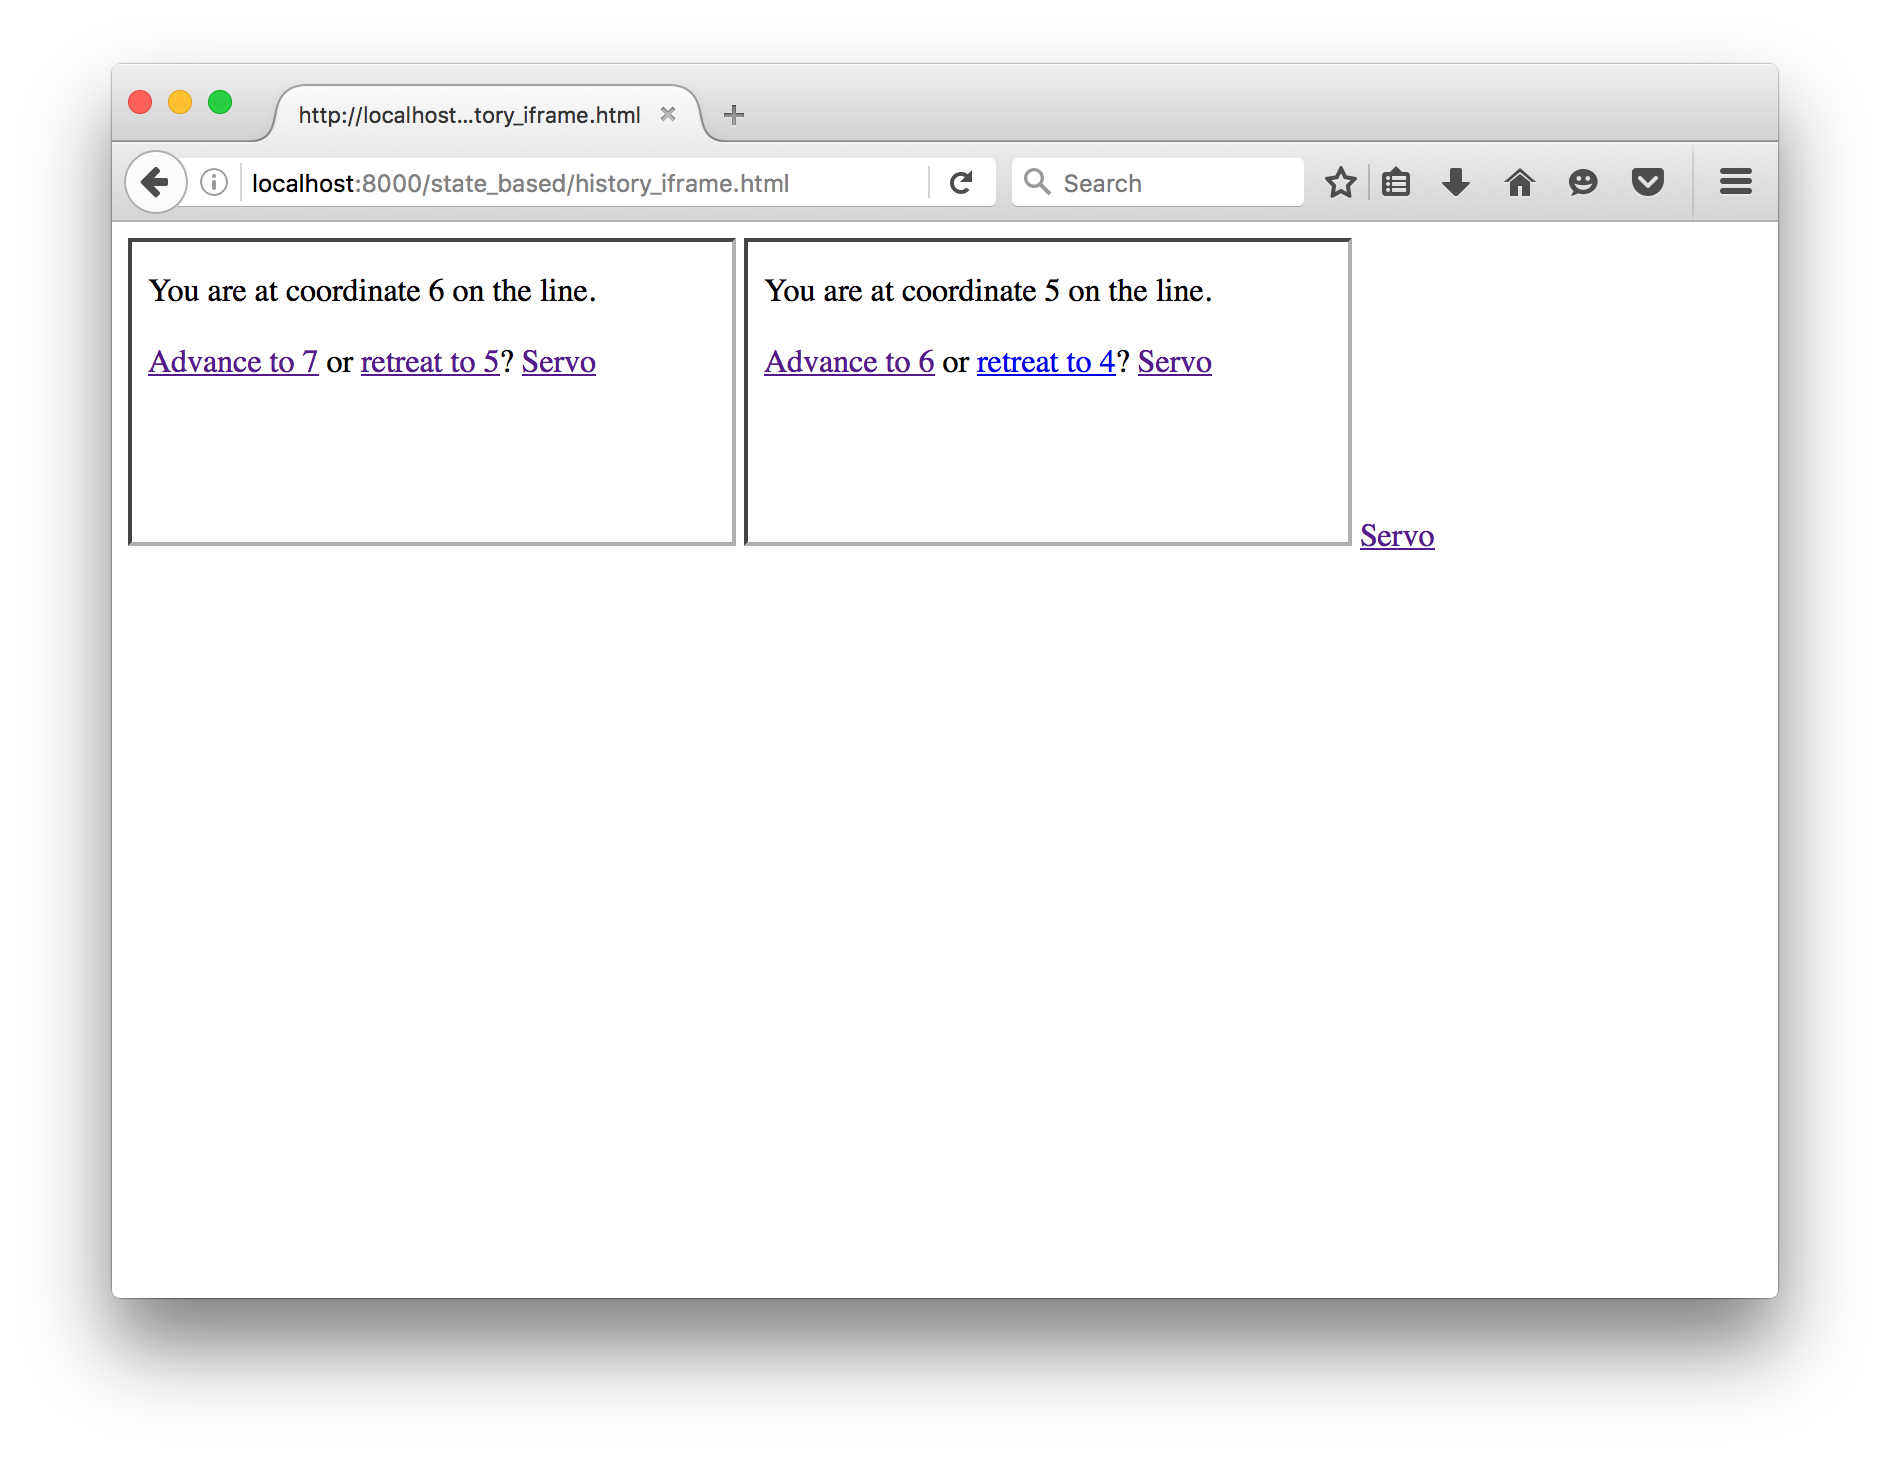
\includegraphics[width=.5\linewidth]{images/experiments/forwardback4state/firefox/2.png}%
    }~\raisebox{-.5\height}{
      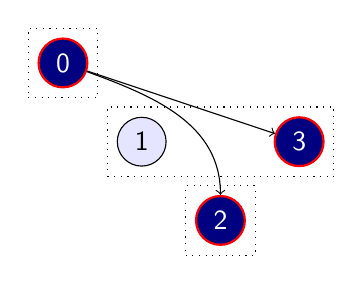
\begin{tikzpicture}
        \node[doc,active,fully](0) at (0,0){0};
        \node[doc](1) at (1,-1){1};
        \node[doc,active,fully](2) at (2,-2){2};
        \node[doc,jshactive,fully](3) at (3,-1){3};
        \node[draw,dotted,fit=(0)]{};
        \node[draw,dotted,fit=(1)(3)]{};
        \node[draw,dotted,fit=(2)]{};
        \draw[->](0)--(3);
        \draw[->](0)to[out=-20,in=90](2);
      \end{tikzpicture}
    }
    \caption{Advance document 1 to $6$}
  \end{figure}

  Advance document 3 to $7$:
  \begin{figure}[H]
    \raisebox{-.5\height}{
      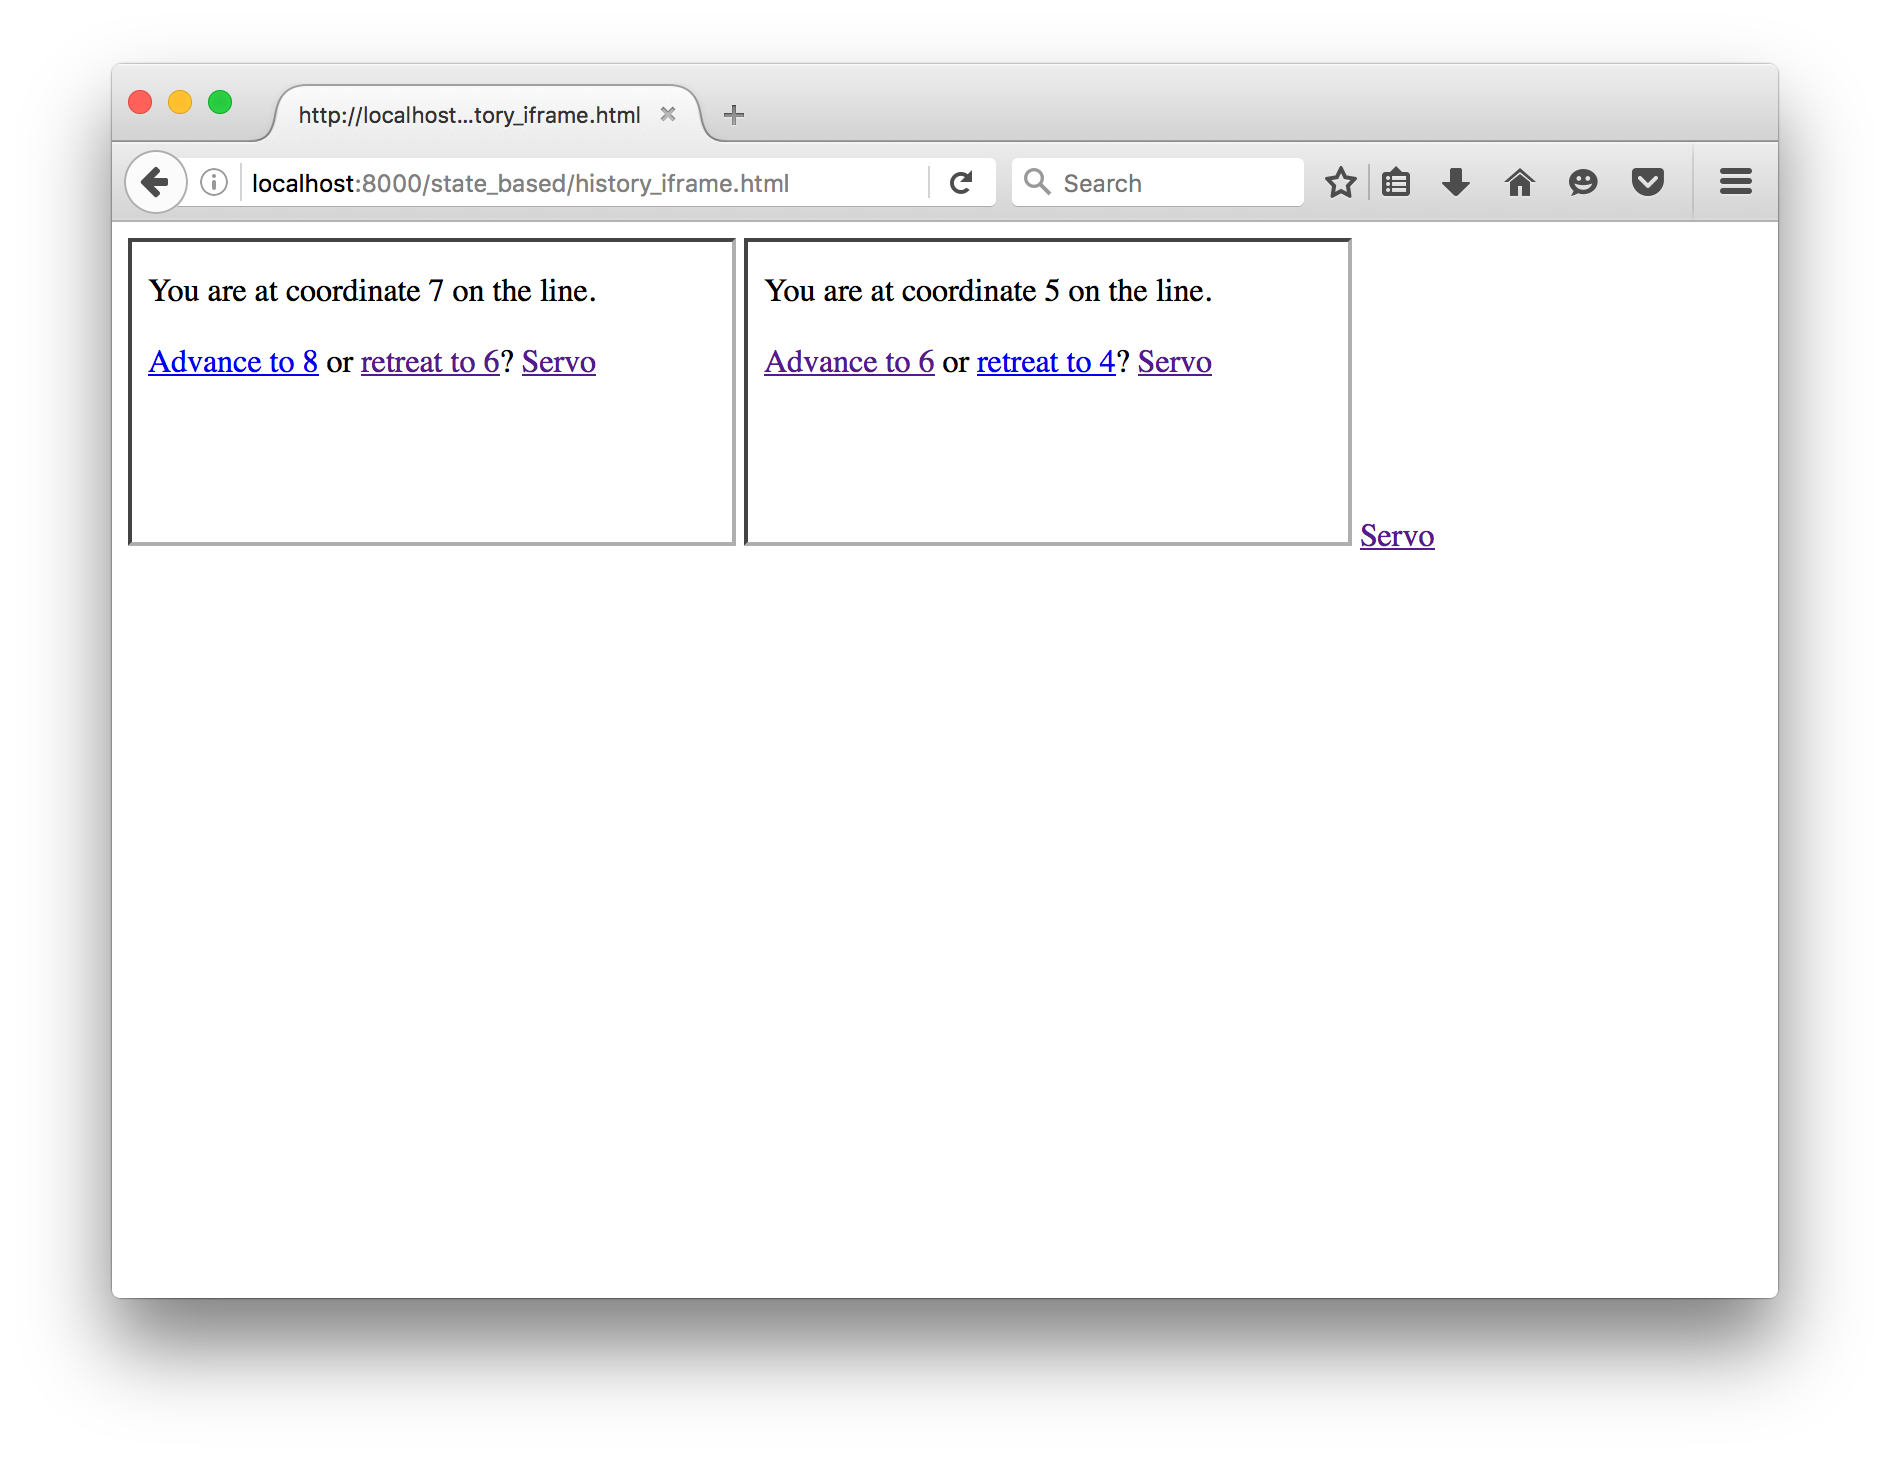
\includegraphics[width=.5\linewidth]{images/experiments/forwardback4state/firefox/3.png}%
    }~\raisebox{-.5\height}{
      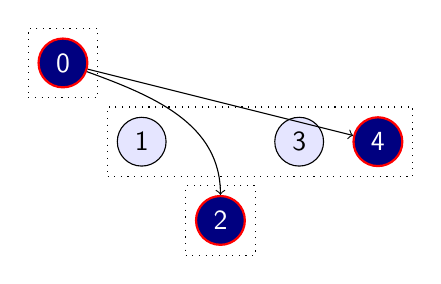
\begin{tikzpicture}
        \node[doc,active,fully](0) at (0,0){0};
        \node[doc](1) at (1,-1){1};
        \node[doc,active,fully](2) at (2,-2){2};
        \node[doc](3) at (3,-1){3};
        \node[doc,jshactive,fully](4) at (4,-1){4};
        \node[draw,dotted,fit=(0)]{};
        \node[draw,dotted,fit=(1)(4)]{};
        \node[draw,dotted,fit=(2)]{};
        \draw[->](0)--(4);
        \draw[->](0)to[out=-20,in=90](2);
      \end{tikzpicture}
    }
    \caption{Advance document 3 to $7$}
  \end{figure}

  Advance document 2 to $6$:
  \begin{figure}[H]
    \raisebox{-.5\height}{
      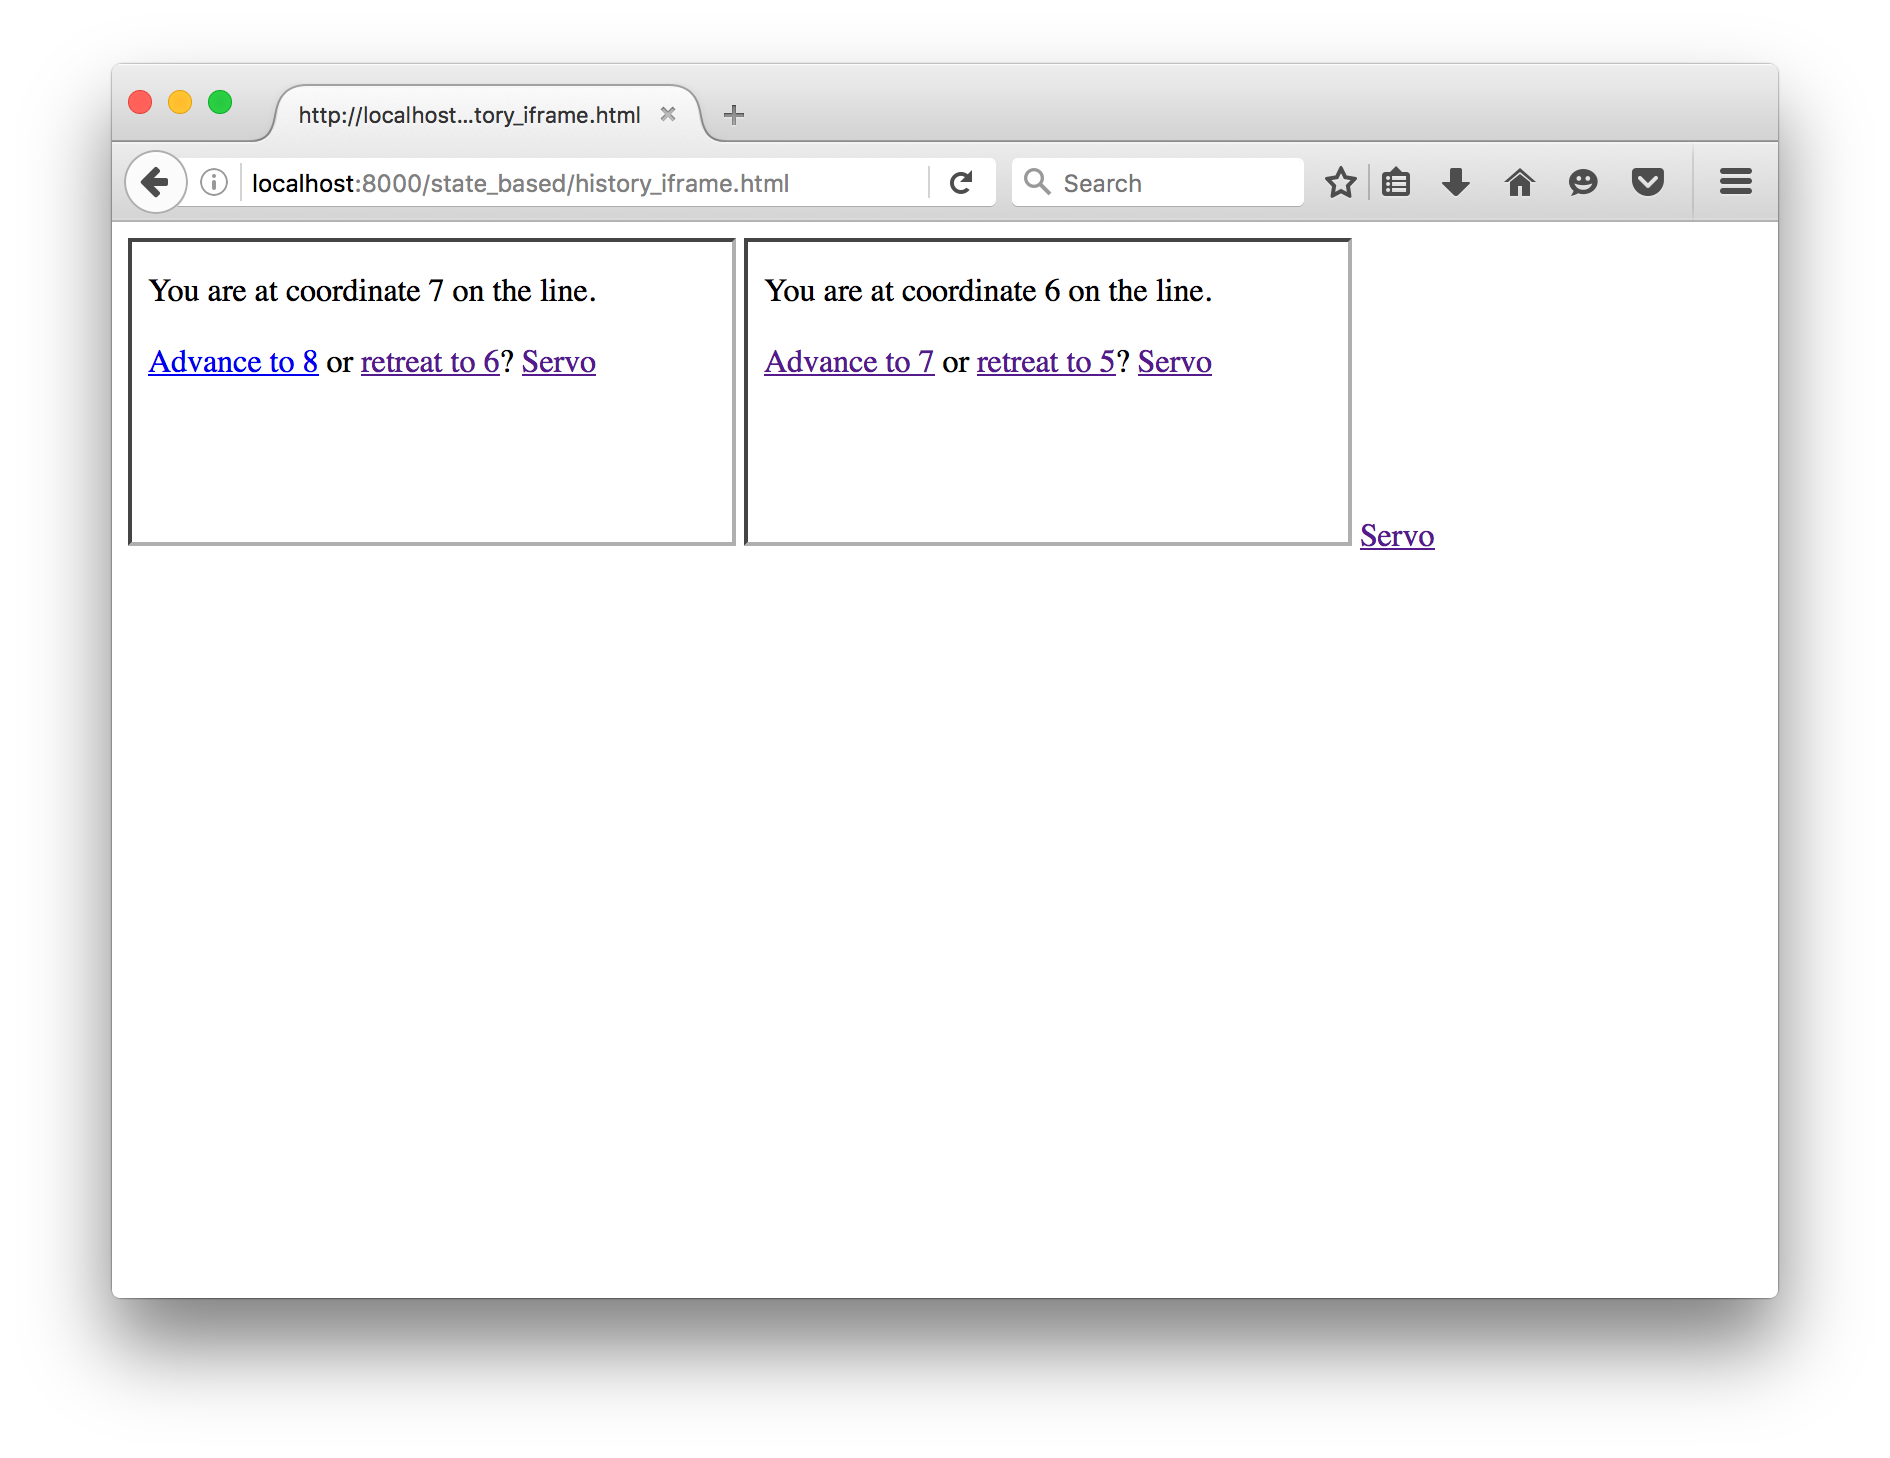
\includegraphics[width=.5\linewidth]{images/experiments/forwardback4state/firefox/4.png}%
    }~\raisebox{-.5\height}{
      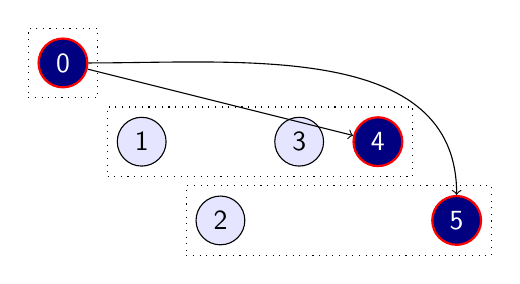
\begin{tikzpicture}
        \node[doc,active,fully](0) at (0,0){0};
        \node[doc](1) at (1,-1){1};
        \node[doc](2) at (2,-2){2};
        \node[doc](3) at (3,-1){3};
        \node[doc,active,fully](4) at (4,-1){4};
        \node[doc,jshactive,fully](5) at (5,-2){5};
        \node[draw,dotted,fit=(0)]{};
        \node[draw,dotted,fit=(1)(4)]{};
        \node[draw,dotted,fit=(2)(5)]{};
        \draw[->](0)--(4);
        \draw[->](0)to[out=0,in=90](5);
      \end{tikzpicture}
    }
    \caption{Advance $document 2$ to $6$}
  \end{figure}

  Advance $document 2$ to $7$:
  \begin{figure}[H]
    \raisebox{-.5\height}{
      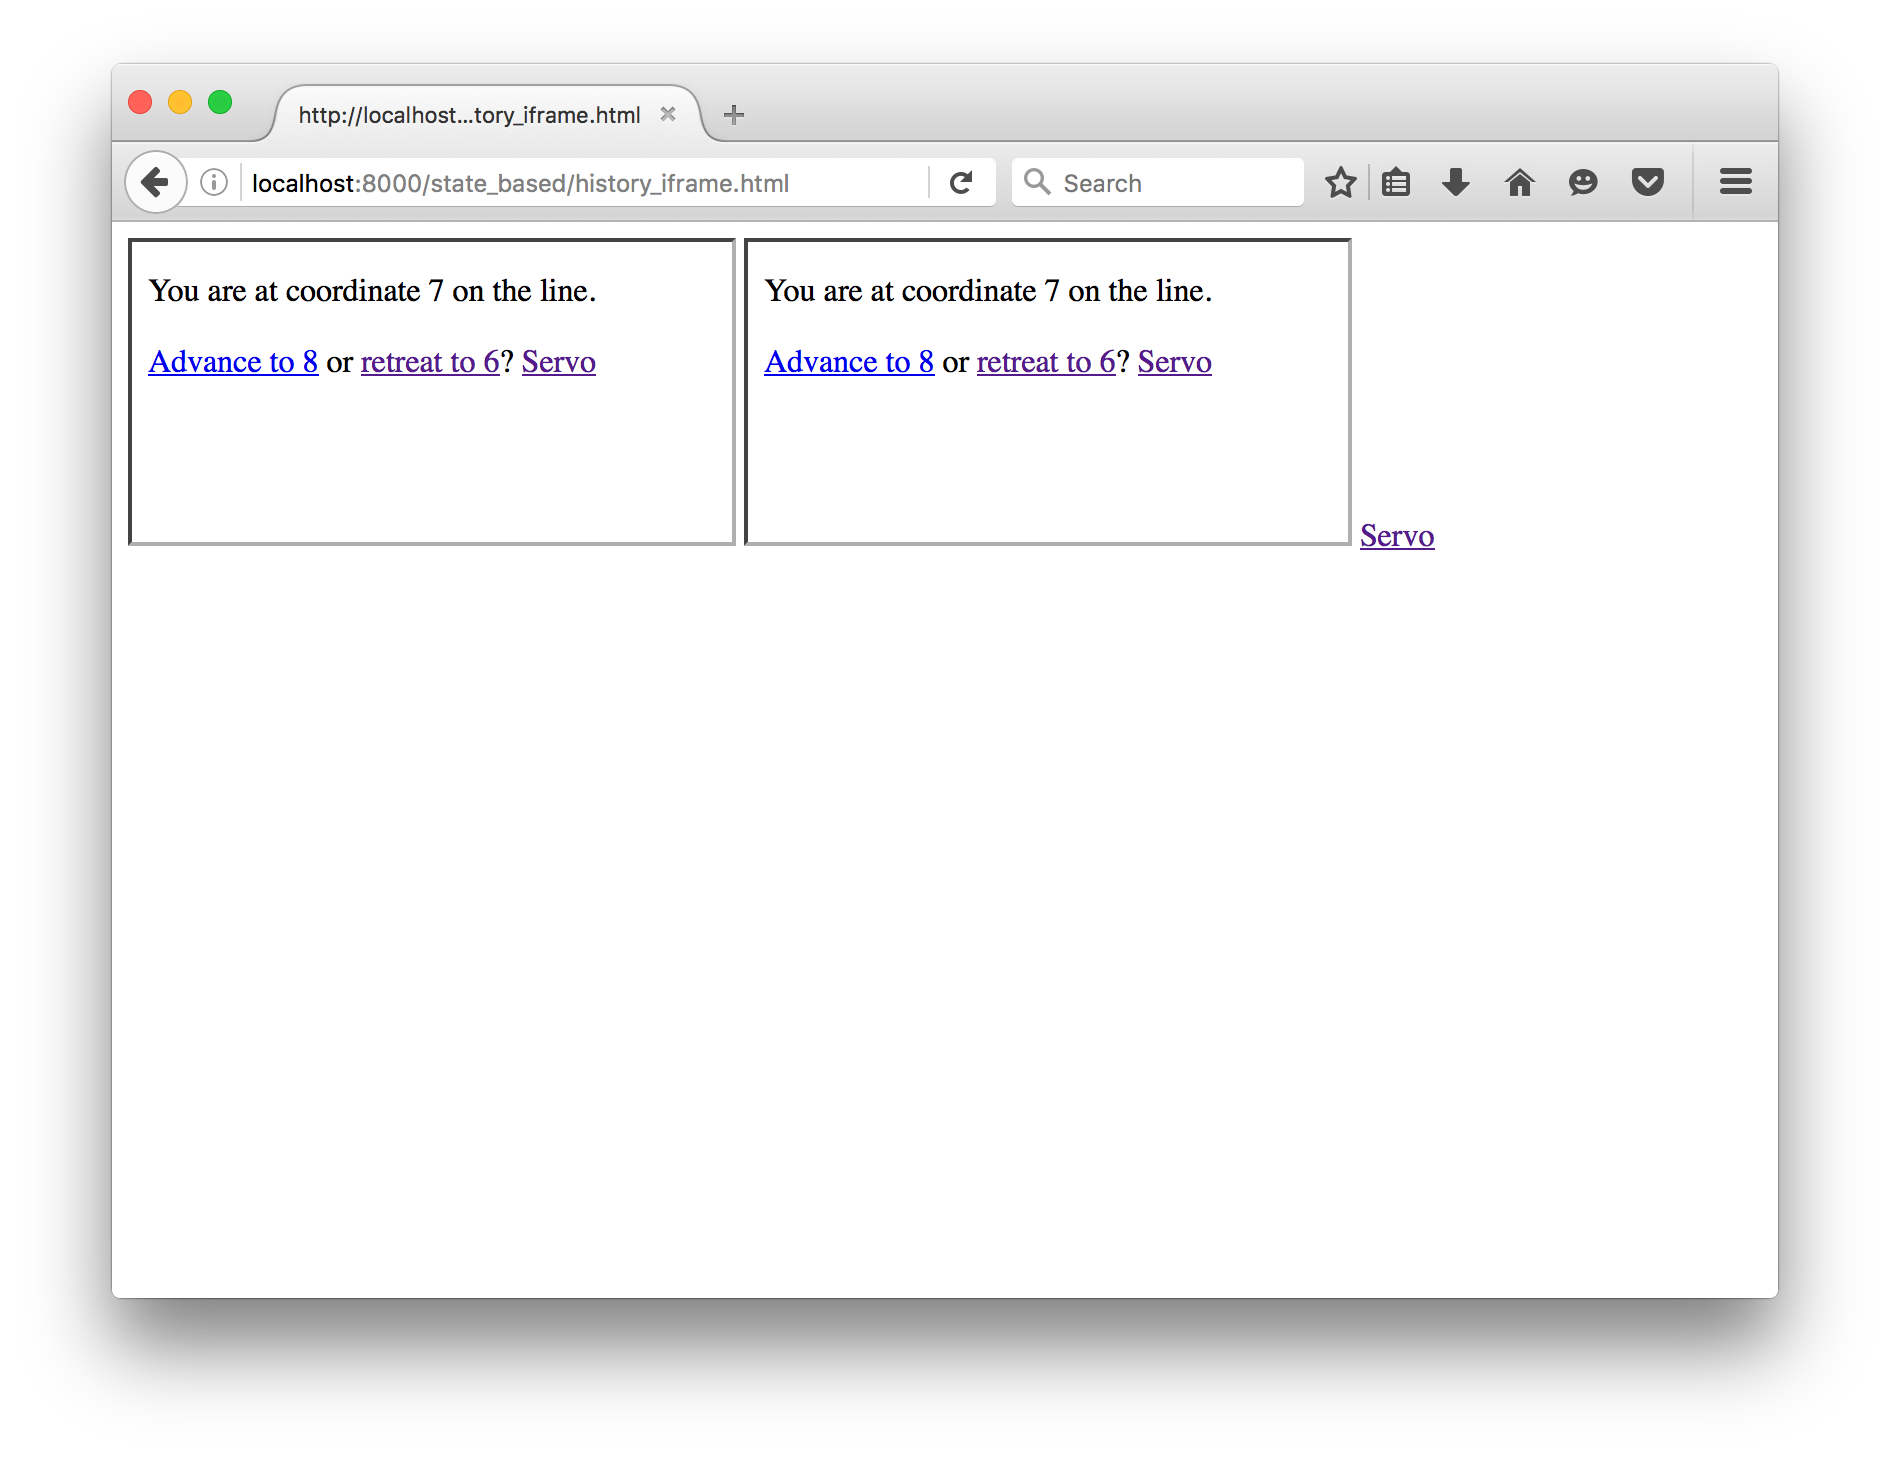
\includegraphics[width=.5\linewidth]{images/experiments/forwardback4state/firefox/5.png}%
    }~\raisebox{-.5\height}{
      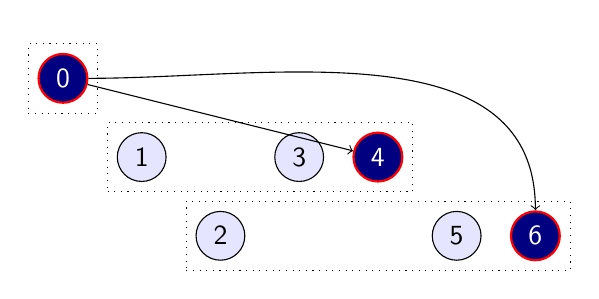
\begin{tikzpicture}
        \node[doc,active,fully](0) at (0,0){0};
        \node[doc](1) at (1,-1){1};
        \node[doc](2) at (2,-2){2};
        \node[doc](3) at (3,-1){3};
        \node[doc,active,fully](4) at (4,-1){4};
        \node[doc](5) at (5,-2){5};
        \node[doc,jshactive,fully](6) at (6,-2){6};
        \node[draw,dotted,fit=(0)]{};
        \node[draw,dotted,fit=(1)(4)]{};
        \node[draw,dotted,fit=(2)(6)]{};
        \draw[->](0)--(4);
        \draw[->](0)to[out=0,in=90](6);
      \end{tikzpicture}
    }
    \caption{Advance document 2 to $7$}
  \end{figure}

  Traverse $\aNH$ by $-4$:
  \begin{figure}[H]
    \raisebox{-.5\height}{
      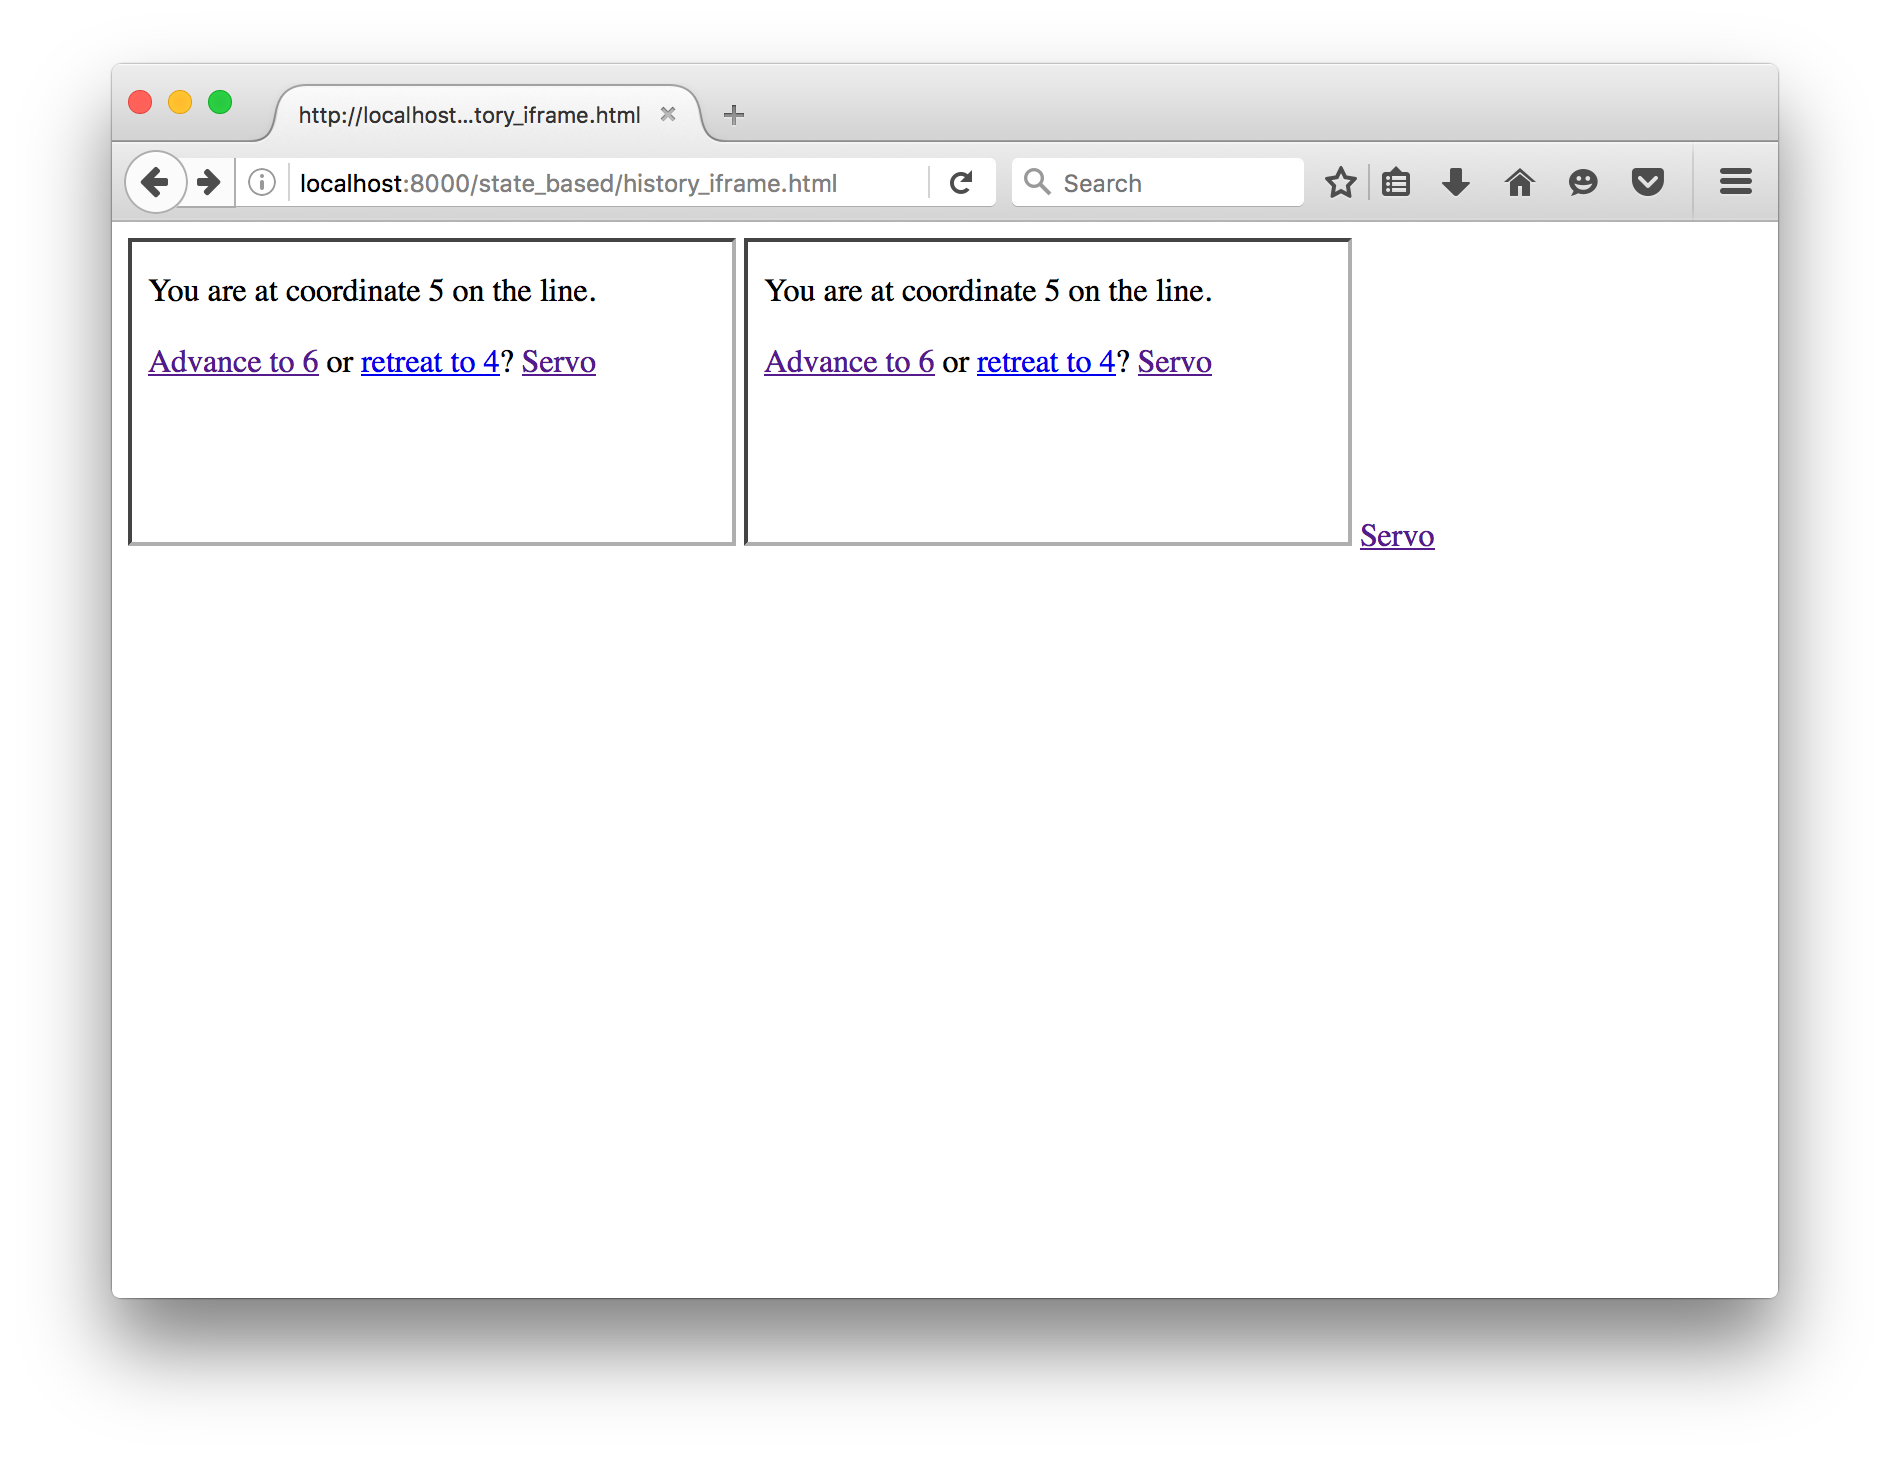
\includegraphics[width=.5\linewidth]{images/experiments/forwardback4state/firefox/6.png}%
    }~\raisebox{-.5\height}{
      \begin{tikzpicture}
        \node[doc,active,fully](0) at (0,0){0};
        \node[doc,active,fully](1) at (1,-1){1};
        \node[doc,jshactive,fully](2) at (2,-2){2};
        \node[doc](3) at (3,-1){3};
        \node[doc](4) at (4,-1){4};
        \node[doc](5) at (5,-2){5};
        \node[doc](6) at (6,-2){6};
        \node[draw,dotted,fit=(0)]{};
        \node[draw,dotted,fit=(1)(4)]{};
        \node[draw,dotted,fit=(2)(6)]{};
        \draw[->](0)--(1);
        \draw[->](0)to[out=-20,in=90](2);
      \end{tikzpicture}
    }
    \caption{Traverse $\aNH$ by $-4$}
  \end{figure}

  Traverse $\aNH$ by $4$:
  \begin{figure}[H]
    \raisebox{-.5\height}{
      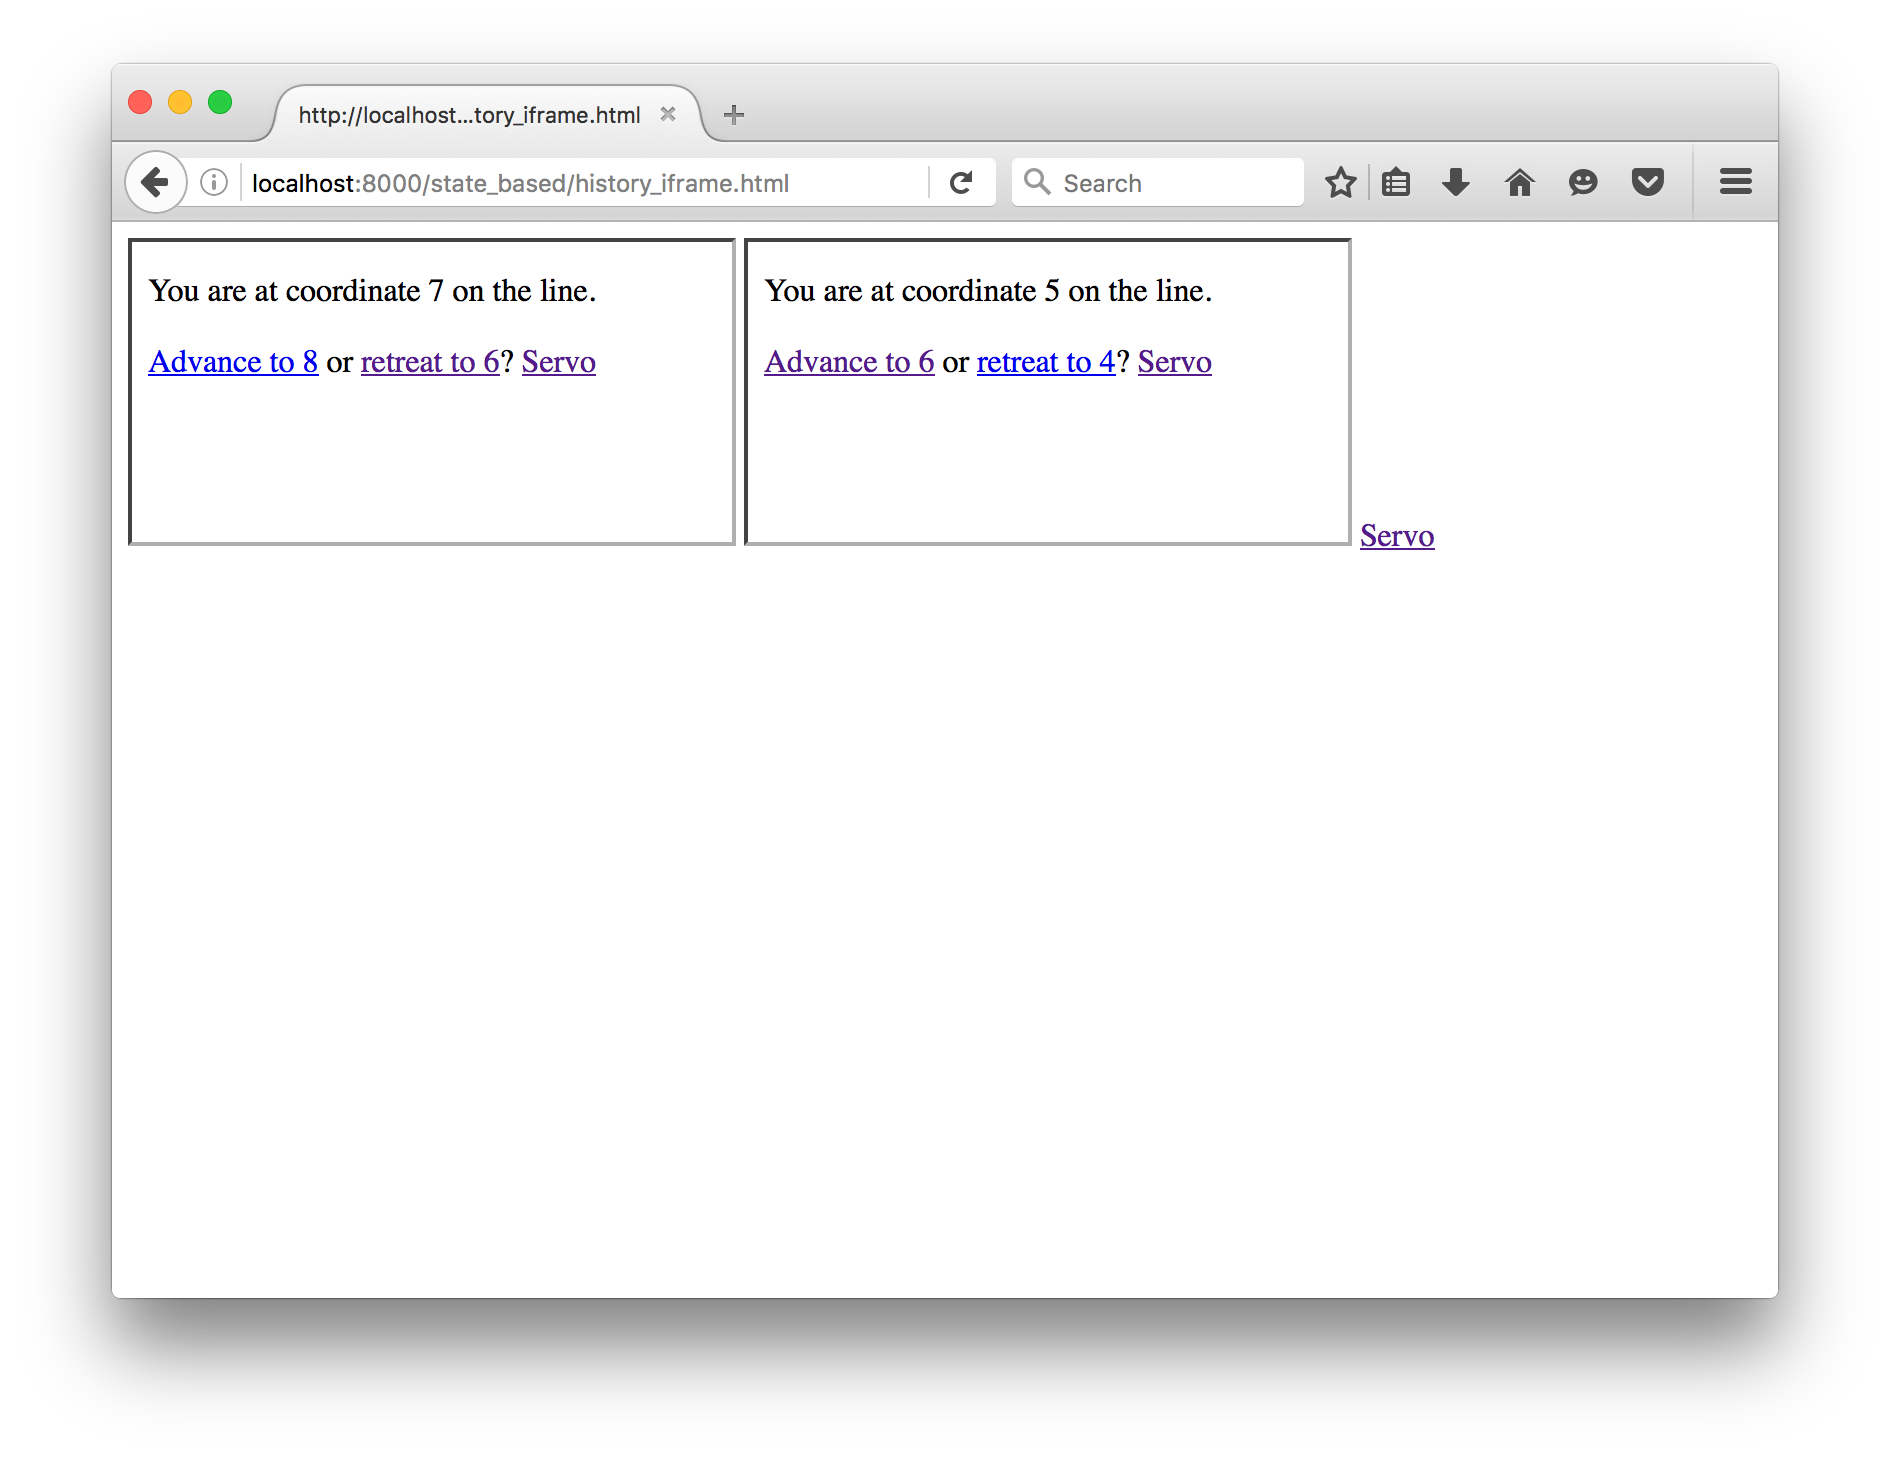
\includegraphics[width=.5\linewidth]{images/experiments/forwardback4state/firefox/7.png}%
    }~\raisebox{-.5\height}{
      \begin{tikzpicture}
        \node[doc,active,fully](0) at (0,0){0};
        \node[doc](1) at (1,-1){1};
        \node[doc,active,fully](2) at (2,-2){2};
        \node[doc](3) at (3,-1){3};
        \node[doc,jshactive,fully](4) at (4,-1){4};
        \node[doc](5) at (5,-2){5};
        \node[doc](6) at (6,-2){6};
        \node[draw,dotted,fit=(0)]{};
        \node[draw,dotted,fit=(1)(4)]{};
        \node[draw,dotted,fit=(2)(6)]{};
        \draw[->](0)--(4);
        \draw[->](0)to[out=-20,in=90](2);
      \end{tikzpicture}
    }
    \caption{Traverse $\aNH$ by $4$}
  \end{figure}

  The last traversal does not satisfy Goal~\ref{goal:homomorphism}.

\end{experiment}

\section{Specification}

[Suggested edits to the spec:
  1. traverse to each document, not just the selected one,
  2. keep all documents in the seession history, not just the fully active ones,
  3. change the session history order.]

\section{Conclusion}

[We did stuff.]

\bibliographystyle{plain}
\bibliography{notes}

\end{document}
